\documentclass[11pt, oneside]{article}   	% use "amsart" instead of "article" for AMSLaTeX format
\usepackage[margin = 1.1in]{geometry}            		% See geometry.pdf to learn the layout options. There are lots.
\geometry{letterpaper}                   		% ... or a4paper or a5paper or ... 
\usepackage[parfill]{parskip}    		% Activate to begin paragraphs with an empty line rather than an indent
\usepackage{graphicx}				% Use pdf, png, jpg, or eps§ with pdflatex; use eps in DVI mode
								% TeX will automatically convert eps --> pdf in pdflatex	
\usepackage{adjustbox}	
\usepackage[section]{placeins}


%% LaTeX Preamble - Common packages
\usepackage[utf8]{inputenc}
\usepackage[english]{babel}
\usepackage{textcomp} % provide lots of new symbols
\usepackage{graphicx}  % Add graphics capabilities
\usepackage{flafter}  % Don't place floats before their definition
\usepackage{amsmath,amssymb}  % Better maths support & more symbols
\usepackage[backend=biber]{biblatex}
\usepackage{amsthm}
\usepackage{bm}  % Define \bm{} to use bold math fontsx
\usepackage[pdftex,bookmarks,colorlinks,breaklinks]{hyperref}  % PDF hyperlinks, with coloured links
\usepackage{memhfixc}  % remove conflict between the memoir class & hyperref
\usepackage{mathtools}
\usepackage[T1]{fontenc}
\usepackage[scaled]{beramono}
\usepackage{listings}
\usepackage{physics}
\usepackage{tensor}
\usepackage{simplewick} 
\usepackage{tikz} 
\usepackage{import}
\usepackage{xifthen}
\usepackage{pdfpages}
\usepackage{transparent}
\usepackage{pgfplots}
\usepackage[compat=1.0.0]{tikz-feynman}
\usepackage{subfiles}
\usepackage{comment} 
\usepackage{fancyhdr}

% fancy formatting
\pagestyle{fancy}
\fancyhf{}

\lhead{An Introduction to Quantum Field Theory}
\rhead{Afiq Hatta}  
%% Commands for typesetting theorems, claims and other things.
\newtheoremstyle{newline}
{\topsep} 
{\topsep} 
{} 
{} 
{\bfseries} 
{}
{.5em}
{\newline}
{}

\theoremstyle{newline} 
\newtheorem{theorem}{Theorem}

\theoremstyle{newline} 
\newtheorem*{thm}{Theorem}

\theoremstyle{newline} 
\newtheorem*{claim}{Claim}

\theoremstyle{newline} 
\newtheorem{example}{Example}

\theoremstyle{newline} 
\newtheorem*{defn}{Definition}

\newcommand{\Lagr}{\mathcal{L}} 
\newcommand{\vc}[1]{\mathbf{#1}}
\newcommand{\pdrv}[2]{\frac{\partial{#1}}{\partial{#2}}}
\newcommand{\thrint}[1]{\int d^3 \vc{x} \left( {#1} \right)}

%% QFT specific macros 
\newcommand{\intp}{ \int \frac{ d^3 p }{ (2 \pi)^3 } \, }
\newcommand{\ann}[1]{a_{ \mathbf{ #1 }}}
\newcommand{\crea}[1]{a^\dagger_{ \mathbf{ #1 }}}
\newcommand{\ve}[1]{ \mathbf{ #1 } } 
\newcommand{\mode}[ 1]{ e^{ i \mathbf{ #1 } \cdot \mathbf{x} }}
\newcommand{\nmode}[1]{ e^{  - i \mathbf{ #1 } \cdot \mathbf{x} }}
\newcommand{\freq}[1]{\omega_\mathbf{ #1} } 
\newcommand{\scal}[1]{\phi ( \mathbf{ #1 })} 
\newcommand{\mom}[1]{ \pi (\mathbf{ #1 })} 
\newcommand{\arr}{\rightarrow} 

\newcommand{\incfig}[1]{%
\def\svgwidth{\columnwidth}
\resizebox{0.75\textwidth}{!}{\input{./figures/#1.pdf_tex}}
}

\newcommand{\anop}[2]{ #1_\mathbf{#2}}
\newcommand{\crop}[2]{#1_\mathbf{#2}^\dagger}

\usepackage{helvet} 

%tikz decoration commands 
\usetikzlibrary{decorations.pathmorphing}


\title{Part III Quantum Field Theory}
\author{Afiq Hatta } 
\begin{document} 

\maketitle

\hypersetup{
    hidelinks=true, 
    colorlinks = false,
    linkbordercolor = {white}
}
\pagebreak 
\tableofcontents

\pagebreak

\section{Why do we care about Quantum Field Theory? } 

If you're reading these set of notes, you've probably done a course at university on basic quantum mechanics. However, there are several philosophical and observed issues in quantum mechanics that we've yet to address. I'll go over them here. 


\subsection{The Problem of Locality} 
\subsection{Particle indistinguishability and Particle conservation}
In quantum mechanics, when we talk about multiparticle systems, we usually tensor product their state representation like $\ket{\psi} \otimes \ket{\phi}$, and we usually don't care about how these things interact. In quantum mechanics, we view particle number as conserved. When we do this however, and attempt to make Schrodinger's equation relativistic, we run into problems with regards to causality violation and unbounded energy. However, in QFT we have multiparticle states, with creation and annihilation operators which remedy this situation. 

\subsection{Problems with QFT} 
In these notes, we'll have a 'free theory' where particles don't interact, and we solve for states analytically. Later, we'll also add on 'interaction terms', where particles do interact and we have to resort to perturbation techniques to study physical quantities of interest. Within these notes, we assume that these interaction terms are small. Physics where we try to understand how to deal with larger interactions is still a big area of research (see lattice QCD where we try to discretise space time and solve QFT numerically). 

\subsection{Scaling in QFT} 
Throughout QFT, we scale out the natural constants $c, \hbar$ to have $c = \hbar = 1$. Because of this, we can form relationship between units of time, length and mass. $c$ is a unit of speed, but since this is set to 1 we have that 
\[ 
[ L ][T]^{-1}  = 1 \implies [L]  = [T] 
\] 
So we have that in this regime, which we call 'natural units' length has units of time. In immediate consequence of this is that energy has the units of mass. 
\[ 
[ E]  = [M] [L]^2 [T]^{-2} = [M] 
\] 
Our condition that the Planck constant goes to 1 implies that \[ 
[ M ][ L]^2 [ T]^{ -1}  = 1 \implies [M ]  = [ L]^{ -1} 
\] 

\pagebreak 
\section{Classical Field Theory} 

\subsection {Euler Lagrange equations for a point particle}  
We'll start off by reviewing some ideas in classical mechanics to motivate our approach to quantum field theory. In particular, the simple harmonic oscillator is a good place to start. In classical mechanics, we describe the motion of a particle $ \mathbf{x}  $ as a function of time, so $\mathbf{x} = \mathbf{x}( t ) $. In high school, we learnt that Newton's laws dictate that in one dimension, mass times acceleration is equal to the force on the particle. So, in the case of the simple harmonic oscillator, \[ m \ddot{x} = - k x \], where $k$ is our spring constant. We then learnt as undergraduates that this is a more specific case of the motion of a particle in a potential $V$, where in the case of a simple harmonic osccilator, $V (x) = \frac{1}{2} k x^2 $. In this formalism, our equations of motion are governed by the equation \[ m \ddot{x} = - \nabla V \] You can check that this recovers the above equation of motion.      

Generalising one step further, we see that we can encode all of this infomation into a single useful quantity, the Lagrangian, which is the quantity $L = T - V$, where $T$ is a kinetic energy term. The Lagrangian should always be a scalar function, and in the case of our harmonic oscilator in 3 dimensions it is \[ 
L = 	\frac{1 } {2} m \dot{ \mathbf{x}}^ 2 - \frac{1}{ 2} k \mathbf{x}^2 \]   
To derive the equations of motion, we want to apply the principle of least action. This principle is that the particle will move along a path which minimises the integral of the Lagrangian over time. In other words, to find out the path of the particle between to points in time, say $t_1$ and $t_2$, we would like to minimise the action.
\[ S = \int_{t_1}^ {t_2} L( \mathbf{ x} , \dot{\mathbf{x} } )   dt \] 
A condition that we impose here is that the endpoints should be fixed, so $\mathbf{x}( t_1 ) = \mathbf{ x} _1$, and $ \mathbf{x}( t_2 ) = \mathbf{x}_2 $.  
To minimise the action, we vary the curve a tiny bit by sending $\mathbf{x} \rightarrow \mathbf{x} + \delta \mathbf{ x} $. This also induces a variation in $\dot{\mathbf{x} } $. We use the chain rule with respect to the variables $\mathbf{x} $ and $\dot{\mathbf{x}} $ and to give \[ 
\delta S = \int_{ t_1}^{t_2} \delta \mathbf{x} \cdot \frac{ \partial L}{ \partial \mathbf{x} } + \delta \dot{\mathbf{x}}\cdot  \frac{ \partial L }{ \partial \dot{\mathbf{x}}} \] 
But, we can perform integration by parts on the second term, by integrating the $\delta \dot{\mathbf{x}} $ and differentiating in the integrand. This gives us a surface term which we can push to zero.
\[ \delta S = \big [ \delta \mathbf{ x} \cdot \frac{ \partial L } { \partial \dot{\mathbf{x}}}   \big ]^{t_2}_{t_1 }  + \int_{t_1}^{t_2} dt \, \, \delta \mathbf{x} \cdot \left( \frac{ \partial L }{ \partial \mathbf{x}} - \frac{d}{dt} \left( \frac{ \partial L }{\partial \dot{\mathbf{x}}} \right) \right)   \] 
Now, since our variation was arbitrary, we have that the integrand needs to be zero, so we have the Euler-Lagrange equation \[ \frac{ d} {dt } \left( \frac{ \partial L } { \partial \dot{ \mathbf{x}} } \right) = \frac{ \partial L }{ \partial \mathbf{x} } \] 

\subsection{Promotion of Point Particles to the Classical Field} 
Previously, we were formulating our problem in a point particle sense. We now alter the physics slightly. Instead of a point particle, suppose we assign a value to every point in spacetime, and work with that instead. This function $\phi = \phi(x) $, we call a \textbf{field}. We write $\phi( x)$ synonymously with $\phi ( \mathbf{x} , t) $. In this regime, much like how we previously viewed $i$ as a label for a spatial coordinate in $x^i$, we now have 
\textbf{infinite degrees of freedom}, where now the $\mathbf{x}$ term in $\phi( \mathbf{x}, t)$ acts as a continuous, infinite label. In essense, fields are like coordinates but with infinite degrees of freedom. In fact, we don't have to stop there. 

We can attach components to this field, thus adding a few more degrees of freedom, and indexing them like $\phi_a ( \mathbf{x}, t)$. So, if we have $a$ indexing over $a =0, 1, 2, 3$, then we've added an additional four degrees of freedom. 

Our most familiar example of this are the electromagnetic fields (which yield 6 degrees of freedom in all). These are $E_i( \mathbf{x}, t)$ and $B_i( \mathbf{ x}, t)$ where our index labels spatial directions. These six fields are derived from the familiar electromagnetic vector potential $A_\mu  = (\phi, \mathbf{A} ) $, given by the following 
\begin{align*}
E_i &=  - \frac{ \partial A_i }{ \partial t }  - \frac{ \partial A_0 }{ \partial x^i} \\
B_i & = \epsilon_{ ijk } \frac{ \partial A_k}{ \partial x_j } 
\end{align*} 


Since we have a field over space now, our Lagrangian itself needs to be an integral over space. So, we formulate our problem in terms of something we call the Lagrangian density. \[ L = \int d^3 x \, \mathcal{L} ( \phi, \partial_\mu \phi ) \] 
where our density now is a function of both the field itself and also the first derivative (not so different from the point particle case). And, like the point particle case, our action is once again the integral over time so that \[ S = \int dt \, L  = \int dt \int d^3 x \, \mathcal{L } = \int d^4 x \, \, \mathcal{ L } \] 
Our Euler Lagrange equations are derived in the same way, but in this case over the 4 space-time coordinates, not just the time coordinate like we did earlier. Our change in action is 
\begin{align*} 
\delta S &= \int d^4 x \, \delta \phi \frac{ \partial \mathcal{ L} }{ \partial \phi } + \delta \partial_\mu \phi \frac{ \partial \mathcal{ L }}{ \partial ( \partial_\mu \phi ) } \\ 
&= \int d^4 x \, \delta \phi \frac{ \partial \mathcal{L } } { \partial \phi }   - \delta\phi  \partial_\mu \frac{\partial \mathcal{ L  }}{ \partial ( \partial_\mu \phi ) }
\end{align*} 
And since our variation $\delta S = 0$, we have the Euler-Lagrange equations 
\[ \partial_\mu  \left( \frac{ \partial \mathcal{ L } }{ \partial (\partial_\mu \phi) } \right)  = \frac{ \partial \mathcal{ L } }{ \partial \phi }  \] 

\subsubsection{The Klein Gordon field} 
We'll now introduce one of the main equations for a free field theory, the Klein-Gordon field. The Klein-Gordon field looks roughly like a Lagrangian for a simple harmonic oscillator
\[ 
\mathcal{L}  = \frac{1}{2} \eta^{ \mu \nu} \partial_\mu \phi \partial_\nu \phi  - \frac{1}{2} m^2 \phi^2 
\] 
$\eta^{\mu \nu}$ denotes our Minkowski metric, which in the course of these notes we'll take to be the 'mostly negative' metric $\eta^{\mu \nu}  = diag ( +1, -1, -1, -1)$. In terms of time and spatial derivatives, our Lagrangian reads 
\[ 
\mathcal{ L }  = \frac{1}{2} \dot{ \phi}^2  - \frac{1}{2} ( \nabla \phi)^2  - \frac{1}{ 2} m^2 \phi^2 
\]

Which is reminiscent of our Lagrangian being of the form $L = T - V$, where $T = \frac{1}{ 2} \dot{ \phi}^2 $ is our kinetic term and the rest is our potential term. We can compute our equations of motion from this. We have that 
\[ 
\frac{ \partial \mathcal{L} }{ \partial \phi} = m^2  \phi, \quad \frac{ \partial \mathcal{ L }}{ \partial ( \partial_\mu \phi ) }  = \partial^\mu \phi 
\] 
where we've used the chain rule for differentiation both times. Substituting this into the Euler-Lagrange equations, we have the Klein-Gordon equation which reads 
\[
\partial_\mu \partial^\mu \phi  - m^2 \phi  = 0 
\]
If we have an ansatz for a plane wave solution, that $\phi(x)  = e^{ - i p \cdot x}$, then this yields the relataivistic dispersion relation that 
\[
p^\mu p_\mu = m^2 
\] 
which we know is true.

\subsubsection{The Lagrangian for Electromagnetism} 
Another important example of a Lagrangian we'll be encountering is the Lagrangian associated with electromagnetism. This is given by 
\[ 
\mathcal{L}  =  - \frac{1}{2} ( \partial_\mu A_\nu)( \partial^\mu A^\nu )   + \frac{1}{ 2} ( \partial_\mu A^\mu)^2 
\] 
where $A^\mu$ is our familiar vector potential we described earlier. Notice that this Lagrangian doesn't depend on $A^\mu$, so if we want to figure out the equations of motion we need to calculate the term $ \frac{ \partial \mathcal{L} } {\partial (\partial_\mu A_\nu) } $. Using the identity that 
\[ 
\frac{ \partial (\partial^\alpha A^\beta) }{ \partial_\mu A_\nu } = \eta^{ \alpha \mu} \eta^{ \beta \nu } 
\] our use of the product rule gives us that 
\begin{align*} 
\frac{ \partial \mathcal{L}}{\partial ( \partial_\mu A_\nu ) } & = - \partial^\mu A^\nu + \partial_\rho A^\rho \frac{ \partial ( \partial_\alpha A^\alpha ) }{ \partial ( \partial_\mu A_\nu ) }   \\
&=  -\partial^\mu A^\nu + \partial_\rho A^\rho \eta\indices{_\alpha^\mu} \eta\indices{^\alpha^\nu} \\
&=  -\partial^\mu A^\nu + \partial_\rho A^\rho \eta^{ \mu \nu } 
\end{align*} 

Our Euler Lagrange condition implies that 
\[ 
0 = \partial_\mu (  - \partial^\mu A^\nu)  + \partial^\nu \partial_\rho A^\rho = \partial_\mu (  - \partial^\mu A^\nu + \partial ^\nu A^\mu ) 
\] 
where in the second term, we relabelled the summed over indices from $\rho \rightarrow \mu$ because they're dummy indices.  
za
\subsection{Lorentz invariance} 
In QFT and special relativity, theories should be invariant under Lorentz transformations. In this section, we will consider active transformations, where we're changing the direction of the field under a Lorentz boost. Under a Lorentz boost, our scalar field $\phi$ changes like 
\[
\phi(x) \rightarrow \phi'(x)  = \phi (x')  = \phi(\Lambda^{ - 1} x ) 
\] 
This is what we call an \textbf{active transformation} since our field is actually, physically shifted.
We're shifting our field by a Lorentz boost in our frame, with $x \rightarrow \Lambda x  $ which induces a change $\phi(x) \rightarrow \phi' (x)$, but this change is equivalent to rotation our frame of reference in the opposite direction first (I'll show a diagram below). 
Our Lorentz boosts are defined by the property that 
\[
\Lambda\indices{^\mu_\rho} \eta^{\rho \tau} \Lambda \indices{_\tau^\nu} = \eta^{ \mu \nu } 
\] 
Lorentz boosts can simultaneously represent rotations in 3-space, as well as boosts in a particular axis in which mixes time and space. For a rotation, our boost is represented as 
\[ 
\Lambda\indices{^\mu_\rho} = \begin{pmatrix} 
1 & 0 & 0 & 0 \\
0 & 1 & 0 & 0 \\
0 & 0 & \cos \theta &  - \sin \theta \\
0 & 0 & - \sin \theta & \cos \theta 
\end{pmatrix} 
\]  
and for a boost, Lorentz transformations are represented by 
\[ 
\Lambda\indices{^\mu_\rho}  = \begin{pmatrix} 
\gamma &  - \gamma v & 0 & 0 \\
- \gamma v & v & 0 & 0 \\
0 & 0 & 1 & 0 \\
0 & 0 & 0 & 1 
\end{pmatrix} 
\] 

In terms of group theory, Lorentz transformations are representations of the Lie group $SO( 3, 1)$ on scalar fields. Let's look at Lorentz invariant theories, which are theories where our physical action $S$ is unchanged by Lorentz transformations. Consider the action 
\[ 
S = \int d^4 x \, \partial_\mu \phi \partial^\mu \phi + U ( \phi(x) ) 
\]
We've declared here that $U ( \phi (x) )$ is some polynomial of $\phi(x)$.  
How does this object change under transformations of our field $\phi( x)  \rightarrow \phi ' ( x) $? Let's do the polynomial term first. Under the active transformation $ \phi(x) \rightarrow \phi' (x) = \phi ( x' )$, we have that 
\[ 
U ( x)  = U ( \phi (x) ) \rightarrow U ( \phi' (x) ) = U ( \phi (x') ) = U ( x') 
\]
This means that $U (x) \rightarrow U ( x')$. Now, to do the kinetic part of the Lagrangian.  
To do this, we observe that our partial derivative of a field transforms as 
\[ 
\partial_\mu \phi \rightarrow \partial_\mu \phi'( x ) = \partial_\mu \phi(x' )  = (\Lambda^{-1} )\indices{^\rho_\mu} \partial'_\rho \phi(x'), \quad x'  =\Lambda^{ -1} x 
\] 
Something important to note here is that we're \textbf{ not} transforming $x$ simultaneously here as well, since this is an active transform of the actual field. We've only expressed $x$ diffferently to express our change in our field in terms of new coordinates, but the same function. 
Thus, our Kinetic term transforms as 
\begin{align*}
\frac{1}{2} \eta^{ \mu \nu} \partial_\mu \phi \partial_\nu \phi & \rightarrow \frac{1}{2} \eta^{ \mu \nu} \partial_\mu \phi' \partial_\nu \phi' \\
&= \frac{1}{2} \eta^{ \mu \nu} ( \Lambda^{ -1})\indices{^\sigma_\mu} ( \Lambda^{ -1} ) \indices{^\tau_\nu} \partial'_\rho ( x' ) \partial'_\tau ( x' ) \\
& = \frac{1}{ 2} \eta^{ \rho \tau} \partial_\rho' \phi(x') \partial_\tau'(x') 
\end{align*} 
where we've used the transformation property of the Minkowski metric. Thus, every term in our Lagrangian density has replaced $x$ with a modified $ x '  = \Lambda^{ -1} x $. We thus have that our action changes like 
\[ 
S = \int d^4 x \, L (x) \rightarrow  S'  = \int d^4 x \, L ( x' ), \quad x' = \Lambda^{ -1}  x 
\] 
However, since the determinant (associated Jacobian) of our Lorentz boost is 1 (as Lorentz boosts are part of the special group $SO(3,1)$, we have that our measure doesn't change: 
\[ 
d^4 x  = det ( \Lambda ) d^4 x'  = d^4 x' \implies S' = \int d^4 x' \, L ( x' )  \implies S = S'
\] 
In the last step we have equality since we're integrating over a dummy variable! Thus, Lagrnagians of this form are Lorentz invariant. 

\pagebreak 
\subsection{Symmetries and Noether's theorem}
We'll now take a look at the role of symmetries in this formalism. In physics, we can have multiple types of symmetries, including Lorentz symmetries, internal symmetries, gauge symmetries and supersymmetries. In terms of Lagrangians, we'll now show that every continuous symmetry of a Lagrangian density gives rise to a conserved current $j^\mu$, which satisfies the conservation condition 
\[ 
\partial_\mu j^\mu = 0 
\]
It's easy to check that, from this quantity, we can construct a conserved charge given by 
\[ 
Q = \int d^3 x \, j^0 
\] 
This is converved with respect to changes in time since 
\[ 
\dot Q = \int d^3 x \, \frac{ \partial j^0 }{ dt }  =  - \int d^3 x \, \nabla \cdot \mathbf{ j } \rightarrow 0 
\] 
where the final term goes to zero, since the divergence theorem allows us to re-express this as a surface integral. We're assuming that $j^\mu (x) \rightarrow 0 $ as $ x^\mu \rightarrow 0$. 
What do we mean by a symmetry? An infinitesimal transformastion of our scalar field 
\[ 
\phi(x) \rightarrow \phi( x)  + \alpha \delta \phi( x) 
\] 
where $\alpha $ is small is a symmetry provided that the Lagrangian only changes by a total four derivative: 
\[ 
\mathcal{L} \rightarrow \mathcal{L } + \partial_\mu F^\mu 
\] 
for some function $F^\mu$. This is a symmetry because since our action integrates over our Lagrangian density, due to the divergence theorem this extra term vanishes, leaving our action $S$ invariant. 
We can now derive Noether's theorem. If we Taylor expand out our Lagrangian, 
\[ 
L(x) \rightarrow L(x) + \alpha \frac{ \partial L }{ \partial \phi} \delta \phi + \alpha \frac{ \partial L}{ \partial ( \partial_\mu \phi ) } \partial_\mu ( \delta \phi )  
\] 
We can rewrite the above term as 
\[ 
L (x) + \alpha \partial_\mu \left( \frac{ \partial L }{ \partial ( \partial_\mu \phi ) }\right)  \delta \phi + \alpha \delta \phi \left( \frac{ \partial L }{ \partial \phi } \right)   - \partial_\mu \left( \frac{ \partial L }{ \partial ( \partial_\mu \phi ) } \right) 
\] 
But, from the Euler Lagrange equations the final term vanishes, and comparing with our total derivative term we find that a conserved current is 
\[ 
j^\mu = \frac{ \partial L }{ \partial ( \partial_\mu \phi ) } \delta \phi  - F^\mu
\] 
Let's consider a Lagrangian with a complex scalar field $\psi$ given by 
\[ 
\psi( x)  = \frac{ 1}{ \sqrt{ 2} } ( \phi_1 ( x) + \phi_2 ( x) ) 
\] 
We treat $\psi ( x)$ and $\psi ( x)^* $ as separate fields, and write a complex scalar lagrangian as 
\[ 
\mathcal{ L } = \partial_\mu \psi \partial^\mu \psi^*  - m^2 \psi^* \psi  - \frac{ \lambda}{2} ( \psi^* \psi)^2 
\] 
It's clear that this Lagrangian is invariant under the phase symmetry 
\[ 
\psi \rightarrow e^{ i \alpha} \psi, \quad \psi^* \rightarrow e^{ - i \alpha} \psi^* 
\] 
This induces the infinitesimal symmetry 
\[ 
\delta \psi = i \alpha \psi, \quad \delta psi^*  = - i \alpha \psi^* 
\] 
With Noether's theorem, one can verify that the conserved current is 
\[ 
j^\mu  = i ( \psi \partial^\mu \psi^ * - \psi^* \partial^\mu \psi )  
\] 

Physically, conserved charges could be anything from conserved electric charge, or conserved particle number such as baryon or lepton number. 
\subsubsection{The Energy-Momentum Tensor} 
In this subsection, we'll be constructing important conserved quantities from Noether's theorem. These conserved quantities will arise specifically from translational symmetry in spacetime. In classical mechanics, energy conservation arose from time translational symmetry, and momentum conservation arose from spatial translational symmetry. In classical field theory, this is no different. Our concept of conserved energy and momentum arise from translational symmetry in our Lagrangian, and we'll combine them to form a single conserved tensor. 
Consider a translation transformation in our spacetime coordinates 
\[
x^\nu \rightarrow x^\nu + \alpha \epsilon^\nu 
\]
We expect that our symmetry here will give rise to a higher rank tensor because we have 4 linearly independent directions arising from $\epsilon^\nu$. Taylor expanding out, we have 
\[
\phi_a(x) \rightarrow \phi_a(x) - \alpha \epsilon^\nu\partial_\nu \phi_a(x)
\]
And this induces a similar transformation on our Lagrangian, since $\mathcal{L} = \mathcal{L} (\phi ( x))  = \mathcal{L}( x)$, so we can Taylor expand our expression in exactly the same way. 
\[ 
\Lagr(x) \rightarrow \Lagr(x)  - \alpha \epsilon^\nu\partial_\nu \Lagr(x) = \Lagr(x) - \alpha \epsilon^\nu \partial_\mu (\delta\indices{^\nu_\mu}\mathcal{L} ) 
\]
In the second expression, we've written things in a slightly weird yet more suggestive manner. Our rationale is as follows. Since $\epsilon^\nu$ has four degrees of freedom, we can write this out as four separate conserved currents as written in the bracket, where the distinct currents are indexed by $\nu$. 
Hence, with Noether's theorem, we can construct four different Noether currents using this form of $\delta \mathcal{L}$. 
\[ 
T\indices{^\mu_\nu} = (j^\mu)_\nu = \partial_\nu \phi_a \frac{ \partial \Lagr }{ \partial_\mu \phi_a}  - \delta\indices{^\mu_\nu}\mathcal{L} , \quad \partial_\mu T^{\mu \nu} = 0 
\] 
Different components of this tensor correspond to different quantities. We have 
\begin{align*} 
\text{Total Energy } & E = \int d^ 3 x T^{ 00} \\
\text{Total momentum } & P^i = \int d^3 x T^{ i0 } 
\end{align*} 
We apply this to our Klein-Gordon field. 
\[ 
\mathcal{L}  = \frac{1}{ 2} \partial_\mu \phi \partial^\mu \phi  - \frac{1} {2}  m^2 \phi^2 
\] 
This has an associated energy-momentum tensor, where raising the index on the delta function yields the Minkowski 
\[ 	
T^{\mu\nu}  = \partial^\mu \phi \partial^\nu \phi  - \eta^{\nu\mu} \mathcal{L } 
\]
Substituting our expression for conserved energy, and momentum 
\[ 
E = \int d^3 x T^{00}  =  \frac{1}{ 2}  \int d^3 x \dot{\phi}^2 + (\nabla \phi)^2 + m^2 \phi^2, \quad P^i  = \int \dot{\phi} \partial^i \phi 
\] 
If $T^{ \mu \nu }$ is non-symmetric, we can massage it into a form that's symmetric which makes it easier to deal with by adding an arbitrary, antisymmetric 'gauge' term 
\[ 
T^{\mu \nu} \rightarrow T^{\mu \nu} + \partial_\rho \Gamma^{ \rho \mu \nu}, \quad  \Gamma^{(\rho \mu) \nu }  = 0
\] This doesn't affect our conservation law, because we have
\[ 
\partial_\mu \partial_\rho \Gamma^{\rho \mu \nu} = 0 
\] 


\subsection{Switching over to the Hamiltonian Formalism} 
In quantum mechanics, we're already used to using the Hamiltonian $H$ to investigate the energy spectrum and energy eigenstates of a system. Right now, we'll build a way to switch over from our current Lagrangian understanding of a scalar field to a derivation of the associated Hamiltonian. To do this, we need to define what conjugate momenta, $ \pi $ is. Conjugate momenta is defined as 

\[ \pi  = \frac{ \partial \mathcal{L} } { \partial \dot{ \phi} } \] 
where $\dot{ \phi } $ is the partial derivative of our field with respect to time. Perhaps some of our intuition about this is as follows. If we were given the Lagrangian $L = \frac{ 1}{ 2} \mathbf{ x} \cdot \mathbf{ x}  - V ( \mathbf{ x} ) $ in the discrete particle case, then our conjugate momenta is given by \[ \pi = \frac{ \partial \mathcal{ L } }{ \partial \dot{\mathbf{x}}} \] which is in this case is $ \dot{\mathbf{x}} $, the expression for our standard notion of momentum with unit mass. 

In the discrete particle case, our Hamiltonian is related to our Lagrangian by a Legendre transform, where \[ 
H = \sum_i \mathbf{\pi} \cdot  \dot{ \mathbf{ x}} - L \] Our sum over $i$ 
denotes the sum of over particles in the system. However, in field theory, we make this continuous by integrating over space instead, and then writing in the Lagrangian density in the integrand. Thus, our expression for the Hamiltonian in field theory is \[ H = \int d^3 x \, \, \pi( x) \phi(x)  - \mathcal{ L } \] 

In the case of the Lagrangian density, we can calculate our conjugate momenta 
\[ 
\mathcal{L}  = \frac{ 1} {2} \dot{\phi}^2  - \frac{1}{ 2} (\nabla \phi)^2  - V( \phi ), \quad \phi  = \dot{\phi} 
\] 
This gives ys an expression for our Hamiltonian density $\mathcal{H}$, which is defined as the integrand of $H = \int d^3 x \mathcal{H} $. 
\[ 
\mathcal{H} = \frac{1}{ 2} ( \pi^ 2 + ( \nabla \phi)^ 2 ) + V(\phi ) 
\] 

Completely analogously to Hamilton's equations in classical dynamics, we have Hamilton's equations defined in terms of partial field derivatives of our Hamiltonian density. 
\[ 
\dot{\phi} = \frac{ \partial  \mathcal{H}}{ \partial \pi }, \quad \dot{\pi} =  - \frac{ \partial \mathcal{H}}{ \partial \phi} 
\] Our Hamiltonian formalism is not obviously a Lorentz invariant theory, but it is!

\subsection{Promoting discrete operators to fields}
We know from standard quantum mechanics how to find the spectrum of the quantum harmonic oscillator $H$ for unit mass, given by 
\[
H  = \frac{1}{2}  p^2 + \frac{1}{2} m \omega^2 q^2. 
\]
$p, q$ represent our momentum and position operators respectively. Last year, we promoted generalised coordinates involving position and momentum to operator values obeying commutation relations. One recalls that we have our canonical commutation relations (which we can derive by examining infinitesimal transformations)
\[ 
[p_a, p_b] = [q_a, q_b] = 0, \quad [q_a, p^b] = i \delta \indices{_a^b}. 
\] 
We can intuitively promote our scalar and momentum fields in the same way, where now a field is an operator valued function of space and time. For simplicity's sake, let's work in the Schrödinger picture where these operators don't depend on time but just space (and we push all our time dependence on states instead)
\begin{align*}
[\phi_a(\mathbf{x}), \pi^b(\mathbf{y})] & = i \delta^3 (\mathbf{x} - \mathbf{y}) \delta\indices{_a^b} \\ 
[\phi_a(\mathbf{x}), \phi^b(\mathbf{y})] &= [\pi_a(\mathbf{x}), \pi^b ( \mathbf{y} ) ] = 0. 
\end{align*}

Our final goal is to compute the spectrum from our Hamiltonian derived from quantum fields. However, this is a hard thing to do. In a free theory however, at any given point in space time, the field evolves independently on other points, and so one useful thing to do is find a basis where we can diagonalise this Hamiltonian. One thing we could do is to Fourier transform $\phi(\mathbf{x} ) $ into momentum space, so that (where we'll put back in our time dependence) 
\[
\phi( \mathbf{x}, t ) = \int \frac{ d^3 x }{ ( 2 \pi )^3 } e^{ i \mathbf{p} \cdot \mathbf{ x} }  \phi( \mathbf{ p }, t ) 
\]
Substituting this into the Klein-Gordon equation by differentiating from within the integrand gives us a simple harmonic oscillator with a momentum dependent frequency, we have the equation 
\[
\left( \frac{ \partial}{ \partial t^ 2 } + ( \mathbf{p}^ 2 + m^2 ) \right) \phi( \mathbf{p}, t ) = 0 
\] This is a simple harmonic oscillator vibrating at frequency 
\[ 
\omega_\mathbf{p} = \sqrt{ \mathbf{p}^2 + m^2 } 
\] So, we have that for a field satisfying the free theory, at every point, we have an infinite superposition of simple harmonic oscillators!

\subsection{Reviewing the Harmonic Oscillator in One Dimension in Quantum Mechanics} 
Going back to the problem of the QM harmonic oscillator, our Lagrangian and Hamiltonian are given by 
\[ 
H  = \frac{1}{2}  p^2 + \frac{1}{2} m \omega^2 q^2, \quad L = \frac{1}{ 2} \dot{ q} ^2  - \frac{1}{ 2} \omega^2 q^2 
\]
Recall that we can reduce our description of the discrete Hamiltonian via creation and annihilation operators, with their important commutation relation 
\[ 
a = \left( \sqrt{\frac{\omega}{2}}  q + i \sqrt{\frac{1}{2 \omega}} p \right), \quad a^{\dagger} = \left( \sqrt{\frac{\omega}{2}}  q - i \sqrt{\frac{1}{2 \omega}} p \right), \quad [a, a^\dagger] = 1 
\] 
We can invert these to give expressions for momentum and position as 
\[ 
q = \frac{1}{ \sqrt{ 2 \omega} } ( a + a^\dagger) \quad, p =  - \frac{ i}{ \sqrt{ 2 \omega} } ( a - a^\dagger) 
\] 
The whole point of the exercise we've done above is to write our Hamiltonian in terms of $a, a^\dagger$, and hence make use of our commutation relations. We can write our Hamiltonian as follows, with the raising and lowering commutation relations
\[ 
H = \omega \left( a^\dagger a + \frac{1}{2} \right), \quad [ H, a^\dagger]  = \omega a^\dagger, \quad [ H, a ] = - \omega a  
\] 
This has the effect of raising and lowering energy eigenstates, which can be shown by applying the Hamiltonian to a raised or lowered state and then using our commutation relations which we derived earlier. 
\begin{align*} 
H a^\dagger\ket{ E} & = ( E+ \omega ) a^\dagger \ket{E} \\
H a \ket{ E}  & = ( E - \omega ) a \ket{E} 
\end{align*} 
Since we can step up or step down energy in this way, we've given rise to a ladder of energy values
\[ 
\dots, E - 2 \omega, E - \omega, E, E + \omega, E+ 2 \omega, \dots 
\] 
There's a caveat here because we can have infinite negative energy! Thus, lowering by $a$ has to stop somewhere. This means that there's a unique state  $\ket{0} $such that 
\[ 	
a \ket{0}  =0 \implies H \ket{ 0 }  = \frac{\omega}{ 2} \ket{ 0 } 
\] We hence have a unique ground state with energy $\omega / 2 $! We call this the zero point energy. Ignoring normalisation, we can step energy up $n$ amount of times by applying raising operators, so that 
\[ 	
\ket{n} = ( a^\dagger)^n \ket{ 0}, \implies H\ket{n}  = (n + \frac{ 1}{ 2})\omega\ket{n} 
\]
In physics however, we usually only care about energy differences, so this non-zero zero point energy is a bit annoying. We apply a procedure called normal ordering, where we reorder terms in an expression so that lowering terms are shoved to the right and raising terms are shoved to the left. The has the notation $: A:$, so in the case of the Hamiltonian 
\[ 	
:H: = \frac{ 1}{ 2} ( : a^\dagger a : + : a a^\dagger: )  \omega  = \omega a^\dagger a 
\]
We now have the effect that our zero point energy is set to zero, with $H\ket{ 0 }  =0 $. We get for free that we can solve for this wavefunction. Since our momentum operator in position space is represented as $p = - i \frac{ \partial}{ \partial q } $, substituting this into $a \ket{0}  = 0$ gives us a differential equation for the state $\ket{0}$ one we contract this in the position basis. 

Rearranging, our expressions for the operators $x, p$ are 
\[ 
x = \frac{1}{\sqrt{2 \omega}} \left( a + a^\dagger \right), p = - i \sqrt{\frac{\omega}{2}} \left( a - a^\dagger \right). 
\] 
This gives rise to commutation relations, which we will show below. 

\subsection{Promoting fields to operators} 
From our definitions for position and momentum operators in the one dimensional case, we can generalise this notion to scalar and conjugate momentum fields. We do this by expanding over all modes, in what looks like a Fourier decomposition. Another motivation for the following definitions is the fact that our operators should be hermitian, which is an extra reason for why we've included terms for both operators.
\[ 
\scal{x}  = \intp \frac{ 1 }{  \sqrt{ 2 \freq{ p}}  } \left( \ann{p} \mode{p}  + \crea{ p} \nmode{p} \right) 
\] 
Again using the form of momentum in 1 dimensional quantum mechanics to motivate definitions, we have a definition for conjugate momentum in terms of Fourier modes as well. This is given by 
\[ 
\mom{x} = \intp ( -i )  \sqrt{ \frac{ \freq{p} }{ 2 } } \left( \ann{p} \mode{p} - \crea{p} \nmode{p} \right) 
\] This procedure is called second quantization, we've reconstructed the scalar and momentum fields completely in terms of and infinite amount of simple harmonic oscillators in momentum space. Again, just as in quantum mechanics, we should impose the commutation relations that 
\[ 
[ \scal{ x}, \scal{y} ] = [ \mom{x},  \mom{y}  ]  = 0, \quad [ \scal{ x}, \mom{y} ] =i  \delta^3 ( \ve{x - y } ) 
\]
However, there's an equivalence here which we'll prove, which is that if we impose that our commutation relations in terms of $\ann{p}$ and $\crea{p}$ as 
\[ 
[ \ann{ p}, \ann{q } ] = [ \crea{p}, \crea{q} ] = 0, \quad [ \ann{p}, \crea{q} ] = ( 2 \pi)^3 \delta^3 ( \mathbf{p - q} ) 
\] then this induces the commutation relations in terms of $\scal{x}$ and $\mom{x}$, and vice versa. 

\begin{thm} 
The commutation relations above are equivalent to each other. 

\begin{proof} 
We'll prove first that the commutation relations on our scalar and momentum fields imply the commutation relations on the annihilation and creation operators. To do do this, we need sensible expansions of these. One can verify with our standard delta function identity that 
\begin{align*} 
\int d^3 x \,  \scal{x} \nmode{p}  &= \frac{ 1}{ \sqrt{ 2 \freq{p } } } \ann{p} +  \frac{ 1}{ \sqrt{ 2 \freq{p } } } \crea{ -p} \\
\int d^3 x \,  \mom{x} \nmode{p} &=  - i \sqrt{ \frac{ \freq{ p}}{ 2} } \ann{p}  + i \sqrt{ \frac{ \freq{ p}}{ 2} }\crea{ p } 
\end{align*} 
Solving this system gives us an expression for $\ann{ p} $. Then, contracting the integral but with $ \mode{p} $ instead gives us $\crea{ p }$. Hence, we have the expressions: 
\begin{align*} 
\ann{p }  &= \sqrt{ \frac{ \freq{ p } }{2} } \int d^3 x   \, \scal{ x} \nmode{ p }  + i \frac{ 1} { \sqrt { 2 \freq{p}}}  \int d^3 x \, \mom{x} \nmode{ p }  \\
\crea{p} &= \sqrt{ \frac{ \freq{p}}{ 2} } \int d^3 x \, d^3 x \, \scal{x} \mode{p}  - i \sqrt{ \frac{ 1}{ 2 \freq{ p }}} \int d^3 x \, \mom{x} \mode{ p } 
\end{align*} 
Now we integrate these over two variables to get 
\begin{align*} 
[\ann{p}, \crea{q} ] & = [  \sqrt{ \frac{ \freq{ p } }{2} } \int d^3 x   \, \scal{ x} \nmode{ p }  + i \frac{ 1} { \sqrt { 2 \freq{p}}}  \int d^3 x \, \mom{x} \nmode{ p }  \\
&, \sqrt{ \frac{ \freq{q}}{ 2} } \int d^3 y \, \scal{y} e^{  i \mathbf{y } \cdot \mathbf{q} }  - i \sqrt{ \frac{ 1}{ 2 \freq{ q }}} \int d^3 y \, \mom{y} e^{i \mathbf{ y} \cdot \mathbf{ q} }  ] 
\end{align*} 
We pull the commutators by linearity into the integral. Now, to make our lives easier, since the scalar fields commute with other scalar fields, and since the momentum fields commute with other momentum fields, we have that the above expression 
\begin{align*} 
[\ann{p}, \crea{q} ]  & =  - \frac{ i }{ 2} \sqrt{ \frac{ \freq{p}}{ \freq {q} } } \int d^3 x d^3 y \,  \nmode{p} e^{ i \mathbf{q} \cdot \mathbf{ y } } [ \scal{x}, \mom{y } ]  + \frac{ i }{ 2} \sqrt { \frac{ \freq{q} } { \freq{p}}} \int d^3 x d^3 y \, e^{ i \mathbf{q} \cdot \mathbf{y } }  \nmode{p} [ \mom { x} , \scal{y} ] \\
&= - \frac{ i }{2}  \sqrt{ \frac{ \freq{p}}{ \freq {q} } } \int d^ 3 x d^3 y\,  i \delta ( \ve{ x - y} ) \nmode{p} e^{  i \mathbf{q} \cdot \mathbf{y } }  + \frac{ i }{ 2} \sqrt { \frac{ \freq{q} } { \freq{p}}} \int d^ 3 x d^ 3 y\,   - i \delta ( \ve{ x -y } ) e^{ i \mathbf{q} \cdot \mathbf{y } } \nmode{p } \\
& = \frac{ 1} { 2} \sqrt { \frac{ \freq{ p } } { \freq{q}}} \int d^3 x\,  \mode{ (q-p)} + \frac{ 1} {2} \sqrt { \frac{ \freq{q}}{ \freq{p}}} \int d^3 x \, \nmode{(p-q)  } \\
&= \frac{ 1}{ 2} \sqrt{ \frac{ \freq{p}} { \freq{q}}} \delta( \ve{ q - p  } ) ( 2 \pi ) ^3  + \frac{ 1}{ 2} \sqrt{ \frac{ \freq{q} } { \freq{p }}} \delta ( \ve{ p - q } ) ( 2 \pi ) ^  3 \\
& = \delta ( \ve{ p - q } ) ( 2 \pi )^ 3, \quad \text{ since } \freq{q} = \freq{ p} \text { when } \ve{p}  = \ve{ q } 
\end{align*} 

Similarly, in the opposite direction, we have that 
\begin{align*} 
[ \scal{x}, \mom{y} ] &= \int \frac{ d^ 3 p d^3 q } { ( 2\pi) ^ 3 } \, ( -i ) \sqrt{ \frac{ \freq{ q } } { \freq{ p } } } \left( - [ \ann{p}, \crea{ q} ] e^{ i \mathbf{ x} \cdot \mathbf{p}  - i \mathbf{ q} \cdot \mathbf{ y } } + [ \crea{ p } , \ann{ q} ] e^{  - i \mathbf{ p } \cdot \mathbf{ x } + i \mathbf{ q} \cdot \mathbf{ y}} \right) \\
& = \intp (  - \frac{ i } { 2} ) \left(  - e^{ i \mathbf{p } \cdot ( \ve{ x - y} ) } - e^{ i \mathbf{ p } \cdot ( \ve{ x -y}  )   } \right) \\
&= i \delta ( \ve{x - y } )  
\end{align*} 
\end{proof} 
\end{thm} 

\subsubsection{Calculating the Hamiltonian} 
Now that we've promoted our scalar and momentum fields as an infinite expansion of annihilation and creation operators, we can start computing objects of interest in terms of Fourier expansions of these operators as well. We'll start by calculating the most important quantity, our Hamiltonian. This is given by, as we calculated earlier, 
\[ H  = \int d^3 x \left( \frac{1}{2} \Pi^2 + \frac{1}{2} \left( \nabla \phi \right)^2 + \frac{1}{2}m^2 \phi^2  \right) \] 
We go term by term, and first calculate the most tricky term
\begin{align*} 
\int d^3 x \, (\nabla \phi)^2 &= \int \frac{d^3 x d^3 p d^3 q}{(2 \pi )^3 } - \frac{1}{2\sqrt{\omega_\mathbf{p} \omega_\mathbf{q}}} \mathbf{p} \cdot\mathbf{q} \left( a_\mathbf{p} e^{i \mathbf{p} \cdot \mathbf{x}} - a_\mathbf{p}^\dagger e^{-  i \mathbf{x} \cdot \mathbf{p}} \right)\left(a_\mathbf{q}e^{i \mathbf{q} \cdot \mathbf{x}} - a_\mathbf{q}^\dagger e^{ - i \mathbf{q} \cdot \mathbf{x}}\right) \\
& = \int \frac{d^3 x d^3 p d^3 q}{(2 \pi )^3 } - \frac{1}{2\sqrt{\omega_\mathbf{p} \omega_\mathbf{q}}} \mathbf{p} \cdot \mathbf{q} (a_\mathbf{p} a_\mathbf{q} e^{i (\mathbf{q} + \mathbf{q}) \cdot \mathbf{x}} \\
& + a_\mathbf{p}^\dagger a_\mathbf{q}^\dagger e^{ - i (\mathbf{p} + \mathbf{q}) \cdot \mathbf{x}}  - a_\mathbf{p}^\dagger a_\mathbf{q}e^{i ( \mathbf{q} - \mathbf{p}) \cdot \mathbf{x}} - \mathbf{q}^\dagger a_\mathbf{p}e^{i (\mathbf{p} - \mathbf{q}) \cdot \mathbf{x}} ) 
\end{align*} But recall that we can integrate over $\mathbf{x}$ first, and make use of the identity 
\[
\int d^3x e^{i \mathbf{a} \cdot \mathbf{x}} = (2 \pi )^3 \delta ( \mathbf{a})
\]
This means that the above expression is equal to 
\begin{align*}
\int d^3 x \, (\nabla \phi)^2&= \int \frac{d^3 p}{(2 \pi )^3} ( - 1) \frac{\mathbf{p} \cdot \mathbf{p}}{2 \omega_\mathbf{p}} \left( a_\mathbf{p} a_{ - \mathbf{p}}  - a_\mathbf{p}^\dagger a_{\mathbf{p}}  - a_{\mathbf{p}}^\dagger a_\mathbf{p} + a_\mathbf{p}^\dagger a_{ - \mathbf{p}}^\dagger \right) \\
&= \int \frac{d^3 p}{(2 \pi)^3 } \frac{ \mathbf{p}^2}{ 2 \freq{ p } }  \left( a_{\mathbf{p}}^\dagger a_{\mathbf{p}} + a_\mathbf{p} a_\mathbf{p}^\dagger \right)
\end{align*}
Going into the second line, we've vanished the first and last terms since the function depends on just the modulus of $p$, but taking the change of variables from $\mathbf{ p} \rightarrow \ve{p} $ means that the expression is equal to the negative of itself. It's easy to show that 
\[\int d^3 \Pi^2  = 0, \quad \int d^3  x \, \frac{ 1}{ 2} m^2 \phi^2 =  \int \frac{d^3 p}{(2 \pi)^3 } \frac{ m^2}{ 2 \freq{ p } }  \left( a_{\mathbf{p}}^\dagger a_{\mathbf{p}} + a_\mathbf{p} a_\mathbf{p}^\dagger \right)  \]
Hence our final expression for our full Hamiltonian is, using the equation for our dispersion relation and commuting the annihilation and creation operators, 
\[
H =  \int \frac{d^3 p}{(2 \pi)^3 } \frac{ \mathbf{p}^2 + m^2 }{ 2 \freq{ p } }  \left( a_{\mathbf{p}}^\dagger a_{\mathbf{p}} + a_\mathbf{p} a_\mathbf{p}^\dagger \right) = \int d^3 p \frac{\omega_\mathbf{p}}{(2 \pi)^3 } \left( a_\mathbf{p}^\dagger a_\mathbf{p} + \frac{1}{2}(2 \pi )^3 \delta (0) \right)
\] 

\subsubsection{Infinity issues with the Hamiltonian} 
Let's calculate the ground state of this Hamiltonian by letting it hit zero, to get $H \ket{ 0 } $. When we hit the annihilation operator in the first term, the term vanishes. Thus, we're only left with the second term. Since $\delta^ 3 ( 0 ) $ is constant, we naively pull this out of the integral to get 
\[ 
H \ket{0 }  = 4 \pi^3 \delta ( 0 ) \int d^3 p\,  \freq{p }, \quad \freq{ p }  = \sqrt{ | \mathbf{ p } |^2 + m^2 }
\] 
However, since we're integrating over all momentum space, we get that $\freq{p} \rightarrow \infty $, and hence the integral diverges (let's ignore the problems associated with the delta function for now)! This is called a high-frequency, or ultraviolet, divergence. However, since we're doing non-gravitational physics, all we care about are energy differences. So, to subtract of this infinity, we could've naively wrote (as similar in the case of the one dimensional harmonic oscillator), that upon reordering of our indices we have that 
\[ 
H = \intp \freq{p } \crea{p} \ann{p} \implies H \ket{ 0 } = 0 
\] So with reordering, we have that zero point energy is just zero. One way to interpret this is that in QFT, we have 'operator ambiguity' in a sense that all operators are defined up to a reordering. Now, we're in a place to properly define normal ordering. 

\begin{defn} 
We denote a normal ordered string of operators, denoted 
\[ 
: \scal{ x_1 } \scal{x_2 } \dots \scal{x_n} : 
\] to be the same operator but with all annihilation operators pulled to the right. 
\end{defn} 
Applying normal operators has the effect of \textbf{removing unwanted infinities} in our expression. It's easy to check that 
\[ 
: H :  =\intp \freq{p } \crea{p} \ann{ p } 
\] 

\begin{thm} 
Our normal ordered Hamiltonian raises and lowers energy as in QM. 
With this definition, our commutation relations with raising and lowering operators are now completely analogous to the case we saw in 1 dimensional QM. 
\[ 
[ H,  \crea{ p } ]  = \freq{p} \crea{ p }, \quad [ H, \ann{ p } ] = - \freq{p } \ann{ p } 
\] 
\begin{proof} 
We substitute in our definitions to find that 
\begin{align*} 
[ H, \crea{ p } ] &= \int \frac{ d^3 q }{ ( 2 \pi )^ 3 } \freq{ q} [ \crea{ q } \ann{q} , \crea{ p } ] \\
& =  \int \frac{ d^3 q }{ ( 2 \pi )^ 3 } \freq{q} \crea{q} [ \ann{ q}, \crea{ p} ] \\
&=   \int \frac{ d^3 q }{ ( 2 \pi )^ 3 } \freq{ q } \crea{ q} ( 2 \pi )^3  \delta ( \ve{ q - p } ) \\
&= \freq{ p } \crea{ p } 
\end{align*} 
The other case is completely similar!
\end{proof} 
\end{thm} 

\subsection{Creating particle states} 
With this framework in mind, we can create excited states with a given energy $\freq{ p }$ from our vacuum by applying raising operators. 
Let's denote $\ket { \mathbf{ p ' } }  = \crea{ p ' } \ket{ 0 } $. Then, applying our Hamiltonian, we have that 
\begin{align*} 
H \ket { \mathbf{ p } '} & = \intp \freq{ p } \crea{ p} \ann{ p} \crea{ p' } \ket{0} \\
&= \intp \freq{ p} \crea{ p } [ \ann{ p }, \crea{ p'} ]\ket{ 0 } \\
&= \freq{ p '} \crea{ p ' } \ket{ 0 } = \freq{  p ' } \ket{ \mathbf{ p }'} 
\end{align*} 
We thus interpret the raised state as  a particle with mass $m$, energy $ \freq{ p' }  = \sqrt{ \ve{ p ' }^2 + m^ 2 }$  and momentum $ \mathbf{ p' } $, where the mass comes from the scalar term $\frac{ 1}{ 2} m^2 \phi^ 2 $ in the Lagrangian. From now on, we will relabel the energy $\freq{ p }$ as $E_\ve{ p } $. From our energy momentum tensor, we could also promote our expression for momentum as an operator, to find that 
\[ 
\ve{ P } =  - \int d^3 x\,  \mom{x} \scal{x}  = \intp \ve{ p} \crea{ p} \ann{ p} 
\] 
One can verify that this definition makes sense by acting on our momentum eigenstate via 
\[ 
\ve{ P } \ket{ \ve{ p}}  = \ve{ p } \ket{ \ve{ p } } 
\] Similarly, constructing our angular momentum operator, $J^i $ as a cross product of our momentum and position operators, to find that for zero momentum eigenstates, $J^i \ket{ \ve{ p } = 0 } = 0 $, in other words, the intrinsic angular momentum, or spin, in zero. Now, to create multi-particle states, we can apply a bunch of raising operators to the vacuum state, and interpret this as a system of multiple particles. 
This is denoted as 
\[ 
\ket{ \ve{ p }_1, \dots \ve{ p} _n }  = \crea{ p_1 } \dots \crea{ p_ n } \ket{ 0} 
\] Because creation operators commute, we have that particles are symmetric under exchange ($ \ket { \ve{ p }, \ve{ q}} =  \ket { \ve{ q}, \ve{ p}})$, which means that this particle species are bosons. 

Our full Hilbert space is then the space of all particles spanned by states of the form $\ket{ 0 }, \crea{p} \ket{ 0 }, \crea{ p } \crea{ q} \ket{ 0 }, \dots $ This is what we call Fock space. We can create another interesting operator on this space, called the number operator, defined as
\[ 
\mathcal{ N }  = \intp \crea{ p} \ann{ p} 
\] This has the property that it counts particle states. This is because since 
\begin{align*} 
\mathcal { N } \ket{ \ve{p_1} \dots \ve{p_n} }  & = \intp \crea{ p} \ann{p} \crea{p_1} \crea{p_2} \dots \crea{ p_n } \ket{ 0} \\
&= \intp \crea{ p} ( [ \ann{ p} , \crea{p_1} ] + \crea{p_1} \ann{ p} ) \crea{p_2} \dots \crea{p_n} [ket{ 0} \\
&= \intp \crea{ p} ( 2\pi )^3 \delta ( \ve{ p - p_1} ) \crea{p_2} \dots \crea{p_n} \ket{0} \\
& + \intp \crea{ p} \crea{ p_1} \ann{p}  \crea{p_2} \crea{p_n} \ket{ 0} \\
&= \ket{ \ve{p_1} \dots \ve{p_n} } + \intp \crea{ p} \crea{ p_1} \ann{p } \crea{ p_2} \dots \crea{ p_n} \ket{ 0 } \\
&= N \ket{ \ve{p_1} \dots \ve{p_n} } 
\end{align*} 
The last line is obtained by repeating the procedure until $\ann{p }$ hits $\ket{ 0}$. 
To show that particle number is conserved in our Fock space, we need to show that this operator commutes with the Hamiltonian. We simply write this out as 
\begin{align*} 
[ H , \mathcal{ N } ] &= \int \frac{ d^3 p d^3 q }{ ( 2 \pi )^6} \freq{q} [ \crea{ q} \ann{q} , \crea{ p} \ann{ p} ] \\
	&=  \int \frac{ d^3 p d^3 q }{ ( 2 \pi )^6} \freq{q} \left( \crea{ q} [ \ann{q}, \crea{ p} \ann{ p} ] + [ \crea{ q}, \crea{ p} \ann{ p } ] \ann{ q} \right)  \\
	&= \int \frac{ d^3 p d^3 q }{ ( 2 \pi )^6} \freq{q} \left( \crea{ q} [ \ann{ q}, \crea{ p } ] \ann{ p} + \crea{ p} [ \crea{ q} , \ann{p} ] \ann{ q}  \right)  \\
&= \int \frac{ d^3 p d^3 q }{ ( 2 \pi )^6} \freq{q} (2 \pi )^3 \delta ( \ve{ p - q} ) \crea{ q} \ann{ p } - (2 \pi )^3 \delta ( \ve{ p - q} ) \crea{ p} \ann{ q} \\
& = 0 
\end{align*} 
Hence we have that the particle operator commutes with the Hamiltonian, and thus the particle number is conserved. 

Note momentum eigenstates aren't localised. We can write a localised state via 
\[ 
\ket{ x} = \intp \nmode{p }  \ket{ \ve{ p} } 
\] More generally, we describe a wave packet partially localised in both position and momentum space. We can write 
\[
\ket{ \psi }  = \intp \nmode{ p } \psi ( \ve { p } ) \ket{ \ve{ p } } , \quad \psi ( \ve { p } ) \propto e^{  - \ve{ p }^2 / 2m^  2 }
\] Neither $\ket { \ve { x} } $ nor  $ \ket { \psi } $ are eigenstates of $H$ like in usual quantum mechanics. 

\subsubsection{Relativistic normalisation} 
From now on, let's define our vacuum state to be normalised such that $ \bra{0}\ket{0}  = 1$. Let's do a simple thing, and just contract two momentum eigenstates, and see what we get; 
\[
\bra{\ve{ p } }\ket{ \ve{ q}} = \bra{ 0 }\ann{ p} \crea{ q } \ket{ 0 }  = \bra{ 0 }[ \ann{p } \crea{ q} ] \ket{0 }  = ( 2\pi )^3 \delta( \ve { p - q} ) 
\]  But, this our delta function Lorentz invariant? If not, it would be in our interest to come up with some expression that is Lorentz invariant, since manifest Lorentz invariance is easy (since things hold in all frames). We know definitely how four momentum transforms under a Lorentz boost, this is just given by
\[ 
p^\mu \rightarrow \Lambda\indices{^\mu_\nu} p^\nu  = p'^\mu 
\] This induces a transformation on our actual \textbf{eigenstates}, where we map $ \ket{ \ve{ p } } \rightarrow \ket{ \ve{ p '} }$.  
In our usual notion of quantum theory, we would want $ \ket{ \ve{ p } } $ to be related to $ \ket{ \ve{ p' } } $ by a unitary transformation, because this forces the contraction to be Lorentz invariant. So we would want 
\begin{align*} 
\ket{ \ve{ p } } \rightarrow \ket{ \ve{ p ' }}  & = U ( \Lambda) \ket { \ve { p }} \\
( 2\pi )^3 \delta( \ve{ p - q} ) &=  \bra{ \ve { p } }\ket{ \ve { q } }  \rightarrow \bra{ \ve{ p } }U^\dagger( \Lambda ) U ( \Lambda ) \ket{\ve{ p } }  = \bra{ \ve{ p ' }}\ket{ \ve{ q' } }  = (2 \pi )^3 \delta ( \ve{ p' - q' } ) 
\end{align*} 
But we can'y assume that this holds in our quantum field theory case - we've made no study into how states change under relativistic transformations. So, the best we can do is to start from a different perspective, and use objects we know which are Lorentz invariant to construct a Lorentz invariant dot product. 

Notice that our identity transformation
\[ 
1 = \intp \ket{\ve{ p } }\bra{ \ve { p } } 
\] is Lorentz invariant, despite the individual states $\ket { \ve{ p } } $ not being Lorentz invariant. This means that or integration expression, or \textbf{measure}, is not Lorentz invariant. Thus, a good place to start is to find a Lorentz invariant measure.

\begin{thm} 
We have that the measure 
\[ 	
\int \frac{ d^3 p}{2 E_\ve{ p } } , \quad E_\ve{ p } = \sqrt { \ve{ p}^2 + m^2 } 
\] is an invariant measure.

\begin{proof}
We construct this item from a chain of Lorentz invariant arguments. First, we assert that the measure 
\[
\int d^4 p 
\] is Lorentz invariant. We know that this is true because when we transform 4-vectors $d^4 p \arr d^4 p'$, the factor is changed by $det ( \Lambda) $. But since Lorentz transformations lie in the special orthogonal group $SO(1, 3)$ this is just 1. In addition. we know that $p^2  = p_\mu p^\mu = p_0^2 - \ve{ p}^2 - m^2 $ is a Lorentz invariant quantity, hence putting this inside a delta function and sticking it inside the integrand also gives us a Lorentz invariant quantity!
So 
\[ 	
\int d^4p \,  \delta \left( p_0^2  - \ve{ p}^2 - m^2 \right) \quad \text{is Lorentz invariant. } 
\] This all seems a bit rabbit-out-of-the-hat at the moment, but bear with us. Let's separate our the time and space terms of our integral like this 
\[
\int d^3 p \int dp_0 \, \delta \left( p_0^2 - \ve{ p}^2  - m^2 \right)  = \int d^3 p \int dp_0 \,  \delta \left( f (p_0 )\right) , \text{ where}  \quad f( p_0) = p_0^2  - \ve{ p} ^2  - m^2 
\] Now, we appeal to an identity we learned in our undergraduate years which allows us to work with delta functions of functions. 
\[	
\delta ( f ( x) )  = \sum_{ x_i } \frac{  \delta ( x - x_i)}{ | f'( x_i) |} \quad \text{ where } x_i \text{ are roots of f }.
\] Now, our roots of $ f$ are at 
\[ 
p_0^{ \pm}  = \pm \sqrt{ \ve{ p }^2 + m^2 } 
\] And, our derivative if just $f' ( p_0 )  = 2 p_0 $. Thus, our full function for our delta function is 
\[	
\delta \left( p_0^2 - \ve{ p}^2  - m^2 \right) = \frac{ \delta ( p_0  -  \sqrt{ \ve{ p }^2 + m^2 }  )}{ 2 \sqrt{ \ve{ p }^2 + m^2 } } +  \frac{ \delta ( p_0  +\sqrt{ \ve{ p }^2 + m^2 }  )}{  2\sqrt{ \ve{ p }^2 + m^2 } } = \frac{ \delta ( p_0  -  E_\ve{ p} )}{ 2 E_\ve{ p}  } +  \frac{ \delta ( p_0  + E_\ve{ p}  )}{  2 E_\ve{ p }  } 
\] Now, we don't have to include both of these delta functions in our integral. It's okay just to choose $p_0 > 0 $, since we cannot Lorentz boost from positive time into negative time. Thus, our notion of sign choice for $p_0$ is also Lorentz invariant. So, selecting just the positive component 
gives us 
\[ 
\int d^3 p \left. \int dp_0 \delta \left( p_0^2 - \ve{ p}^2  - m^2 \right) \right\vert_{p_0 > 0 }  = \,\int d^3 p  \int d p_0 \, \frac{ \delta ( p_0  -  E_\ve{ p} )}{ 2 E_\ve{ p}  } = \int \frac{ d^3 p }{ 2 E_ \ve{ p} } 
\] since the delta function absorbed into the $\int p_0$ just goes to one. 
\end{proof}
\end{thm}  

With this fact, we motivate the concept of a relativistically normalised state; which we denote as 
\[ 	
\ket{ p^\mu }  : = \ket{ p } = \sqrt{ 2 E_\ve{ p } } \ket{ \ve{ p } } 
\] This is manifestly Lorentz invariant because  
\[ 
I = \int \frac { d^3 p }{ 2 E_\ve{p} } \ket{ p }\bra{p } 
\] is Lorentz invariant, and so is the measure. Hence the integrand must be Lorentz invariant. Thus, our normalised delta function looks like 
\[ 
\bra{ p}\ket{ q} = ( 2 \pi )^3 2 \sqrt{ E_\ve{ p} E_\ve{ q} } \delta^3 ( \ve{ p - q} ) 
\] 

\pagebreak
\subsection{Quantising the free complex scalar field} 
Let's explore what we get when we play around with a complex, free-like Lagrangian. We have the Lagrangian attached with a mass term
\[ 
\Lagr = \partial^\mu \psi^* \partial _\mu \psi - \mu^2 \psi^* \psi 
\] This Lagrangian is associated with the following Euler-Lagrange equations 
\begin{align*} 	
\partial_\mu \partial^\mu \psi + \mu^2 \psi &= 0 \\
\partial_\mu \partial^\mu \psi^* + \mu^2 \psi^* = 0 
\end{align*} 
Now since the complex conjugate of our field $\psi$ is not the same as $\psi^*$, when we promote $\psi$ to a Schrodinger picture operator there's no notion which suggests that the operator should be Hermitian. So, we write out a normalised expansion that's similar to what we had for a scalar field but, add different operators inside. We have 
\begin{align*} 
\psi( \ve{ x} ) = \intp \frac{ 1 }{ \sqrt{ 2 E_\ve{p} } } ( \anop{ b }{ p } \mode{p}  + \crop{c}{ p } \nmode{p}) \\
\psi(\ve{ x} )^\dagger  = \intp \frac{ 1 }{ \sqrt{ 2 E_\ve{p} } } ( \crop{b}{ p} \nmode{p}  + \anop{c}{ p} \mode{p} ) \\
\end{align*} In addition, we motivate the same expressions for our conjugate momenta. Our conjugate momenta classically is found by differentiating the Lagrangian: 
\[ 	
\pi = \frac{ \partial \Lagr }{ \partial \dot{ \psi } }  = \dot{ \psi}^* 
\] With the same Heuristic we applied to find conjugate momenta for our scalar field, we tentatively write that 
\begin{align*} 
\pi & = \intp i \sqrt{ \frac{ E_\ve{ p } }{ 2 } } ( \crop{ b }{ p } \nmode{p}  - \anop{c}{ p } \nmode{ p })  \\
\pi^\dagger &= \intp ( -i ) \sqrt{ \frac{ E_\ve{ p} } { 2} } ( \anop{b}{ p} \mode{p}  - \crop{c}{ p} \mode{ p} ) 
\end{align*} Here, we've defined two operators $b, c$, which have the interpretation of creating and annihilating a particle and antiparticle respectively. 
With this expansion one can check that the commutation relations 
\[ 
[ \scal{ x}, \mom{ y } ] = i \delta( \ve{ x - y } ), \quad [ \scal{x}, \mom{ y }^\dagger ]  = 0, \quad \text{ all other relations derived from this } 
\] are equivalent to the commutation relations 
\[ 	
[ \anop{ b }{ p}, \crop{ b }{ q}]  = ( 2\pi) ^3 \delta ( \ve{ p -q } ), \quad [ \anop{ c }{ p}, \crop{ c }{ q}]  = ( 2\pi) ^3 \delta ( \ve{ p -q } ), \quad \text{ all other relations 0 } 
\] We interpret the operators as particle and anti particle creation. These particles have spin 0, and the same mass since we have a $\mu^2 $ coupling term in there. Since a real scalar field obeys $\psi^* = \psi $, our interpretation of a particle created by a real scalar field is that it its' own antiparticle. Using Noether's theorem, one can show that our conserved charge which is obtained by the symmetry of a phase rotation 
\[	
\psi \arr e^{ i \theta} \psi 
\] gives rise to the conserved charge 
\[
Q  = i \int d^3 x \,  \dot{ \psi}^* \psi - \psi^* \dot{ \psi }  
\] Using the relation we derived earlier for conjugate momentum, this can be written as 
\[ 
Q = \int d^3 x\, \pi \psi - \psi^\dagger \pi^\dagger 
\] Expanding this in terms of the creation and annihilation operators $b,c$, with normal ordering we have that a conserved charge is 
\[ 	 
Q  = \intp ( \crop{ c}{ p} \anop{c}{ p } - \crop{ b }{ p } \anop{ b }{ p } ) = N_c - N_b 
\] This counts the number of of particles minus the number of anti-particles. 

\pagebreak

\subsection{Introducing time with the Heisenberg picture}
So far, in the Schrodinger picture, we aren't entirely confident that our operators are manifestly Lorentz invariant. In the Schrodinger picture, operators don't depend on time but states do since the evolve according to the equation 
\[	 
i \frac{ d \ket{ \ve{ p } } }{ dt }  = H \ket { \ve{ p} }  = E_\ve{ p } \ket{ \ve{ p } } 
\] This however, is entirely equivalent to placing time dependence on operators instead of states, and force operators to evolve according to 
\[ 	
O_H( t )  = e^{ i H t } O_s   e^{ - i H t } 
\] where $ O_s $ is our Schrodinger picture operator which coincides with our Heisenberg picture operator at $t = 0$. At a fixed time, substituting this expressions now give us fixed time commutation relations. Recall that 
\[ 	
[ U A U^{ - 1}, U BU^{ - 1} ] = U[ A , B ] U^{ -1 } 
\] Application of this identity yields us the fixed time commutation relations 
\[
[ \phi ( \ve { x} , t ), \phi( \ve{ y } , t ) ]  = [ \pi ( \ve{ x} , t ) , \pi ( \ve{ y}, t ) ] = 0, \quad  [ \phi( \ve{ x}, t ), \pi ( \ve{ y }, t ) ] = i \delta ( \ve{ x -y } ) 
\] 
Taylor expanding out we have 
\[
O_H(t + \delta t ) = 1 + \delta t i[H, O_\mathcal{H} ( t) ] + \dots
\]
so operators obey the Heisenberg equations of motion, that 
\[ 	
i \frac{ d O_H}{ dt }  = i [ H, O_H ] 
\] We can use this to calculate our time derivatives of our operators, to get $\dot{ \pi}$ and $\dot{ \phi } $. We can then relate $\pi = \dot{ \phi } $ to obtain the Klein Gordon equation. For notation purposes, we write 
\[ 
\psi ( x) := \phi( \ve{ x} , t ) \] 
We can check, by computing the commutator $[ a_\ve{ p }, e^{ -i H t } ] $, and $[ a_\ve{ p }^\dagger, e^{ -i H t } ] $, that 
\begin{align*} 
e^{i H t} a_\ve{ p } e^{ - iH t } &= e^{ - i E_\ve{ p} t } a_\ve{ p} \\
e^{i H t} a_\ve{ p }^\dagger  e^{ - iH t } &= e^{ i E_\ve{ p} t } a_\ve{ p} 
\end{align*}   Hence, we have 
\[
\phi ( x)  = \intp \frac{ 1 }{ \sqrt { 2 E_\ve{ p } } } (\ann{p}e^{ -i p \cdot x }  + \crea{ p } e^{ i p \cdot x } ) 
\] 


with this we can calculate $\dot{\phi}$ amd $\dot{\pi}$. (Insert section to check that this recovers the relativistic Klein Gordon equation). 
We promote $\phi(\mathbf{x}), \pi(\mathbf{x})$
to adopt time dependence, so we write 
\[
\phi(\mathbf{x}, t) = \phi(x) 
\] and similiarly with $\pi(x)$. 

Our Hamiltonian which didn't depend on time was\[ H = \int \frac{d^3 x }{(2 \pi)^3} a_{\mathbf{p}}e^{i \mathbf{p} \cdot \mathbf{x}}+ a_{\mathbf{p}}^\dagger e^{-i \mathbf{x} \cdot \mathbf{p}}
\] 
but to calculate the time dependent Hamiltonian we'd need to calculate 
\[ e^{i H t }a_\mathbf{p} e^{ - i H t}, \quad e^{iHt} a_\mathbf{p}e^{ - i H t} \]

The first operator is only non-zero when we contract it on both sides for the configuration 
\[ \bra{0}e^{i H t}a_{\mathbf{p}} e^{ - iHt} \ket{\mathbf{p}},\]  and this gives us 
\[ \bra{0}e^{iH t }a_{\mathbf{p}}e^{- iH t }\ket{\mathbf{p}} = e^{ - i E_{\mathbf{p}} t} \] 
thus our conjugated operator is 
\[ e^{iHt}a_\mathbf{p}e^{ - iHt}  = a_{\mathbf{p}}e^{ -i E_\mathbf{p}t} \] and similarly we have that 
\[ e^{ iHt}a_\mathbf{p}^\dagger e^{ - iHt}  = a_{\mathbf{p}}^\dagger e^{i E_\mathbf{p} t} \] 

Since $ p  = (E_\mathbf{p}, \mathbf{p})$, altogether this gives our expression for our scalar field 
\[
\phi (x) = \int \frac{d^3 x }{(2 \pi)^3} \frac{1}{\sqrt{E_\mathbf{p}}} \left( a_\mathbf{p}e^{ -i p \cdot x} + a_\mathbf{p}^\dagger e^{i p \cdot x} \right) 
\]


\pagebreak 

\section{Causality in QFT} 
We still have that potentially, a hint of Lorentz variance because 
the commutation relations of $ \phi$ and $\pi $ are 
equal time relations. If we shift to a differed time, this
may not hold. Our previous fixed time commutation relations involved expressions of the form 
\[
[ \mathcal{ O}_2( \vec{x}, t ) , \mathcal{O}_1 ( \vec{y}, t ) ]
\] but, if we transform the coordinates with a Lorentz transformation, we would get this turning into
\[
[ \mathcal{ O }_1 ( \vec{x}' , t' ) , \mathcal{ O }_2 ( \vec{y}', t'' ) ]  
\] where $ t' ,  t'' $ are not necessarily the same since $ \vec{x}, \vec{y}$ are different. 
What about arbitrary space time separations? 
The real requirement of causality is that all 
space like separated operators commute 
\[ 	[ \mathcal{ O }( x_1 ) , \mathcal{ O }( x_2) ] = 0 , \quad \forall ( x- y)^2 < 0 
\] The reason why commutation is synonymous 
with the fact that operators don't affect one another, 
comes from the fact that they have a shared eigenbasis. 
Suppose we have $A, B  $, hermitian operators which commute. 
Then, we have that they share an eigenbasis which we label as $ \left\{  \ket{ i }  \right\} $, with the property that 
\begin{align*}
A \ket{ i }  & = \lambda_i \ket{ i }, \quad \lambda_i \in \mathbb { R} \\
B \ket{i } &=  \mu_i \ket{ i }, \mu_i \in \mathbb{ R}  
\end{align*} In particular, this means that 
if we expand a given quantum state in terms of the eigenbasis, we get 
\[
\ket{ \psi }  = \sum_{ i } a_{ i } \ket{ i } \implies \bra{ \psi }BA\ket{\psi}  = \sum_i a_{ i } \lambda_{ i } \mu_{ i}
\] where in the last sum we used the orthogonality property 
of the eigenstates. However, notice that this is the same by symmetry of 
calculating $ \bra{ \psi }AB\ket{ \psi}$. Hence, applying an operator 
in the process of measuring the other one doesn't change our 
outcomes. Thus, we have no causality.

If we define $ \Delta( x -y )  = [ \phi ( x), \phi ( y ) ] $, we'd like to check if this holds for space-time separation.  
\[ [ \phi ( x), \phi ( y ) ]  = 
\int \frac{d^{ 3 } p \, d^ 3 p' }{ ( 2 \pi )^6 \sqrt{ 4 E_p E_p' } } \left\{ [a_{\vec{p}}, a_{\vec{p}'}^\dagger ] e^{ i ( p \cdot  x  - p' \cdot  y) } + [ a_{\vec{p}}^\dagger , a_{\vec{p}'} ] e^{ i ( p \cdot  x - p ' \cdot  y) }   \right\} 
\] which is just 
\[ [ \phi ( x) , \phi ( y ) ] 
= \int \frac{ d^3 p }{ 2 E_p ( 2 \pi )^3 } \left\{ e^{  - i p \cdot  ( x - y ) } - e^{ i p \cdot  ( x - y ) } \right\} 
\] Well, what do we know about this function? 
We know that this is Lorentz invariant because the measure is, and so is the 
integrand. 
If  $ x - y $ is space-like, it vanishes because we can take
a Lorentz transformation to $ y - x$ in the first term, 
giving 0. Another way to say this is that if we have space-like separated events, 
then we don't care about breaching causality in time, so we can freely 
transform events in this way. We can't however do this for 
time like events because that would mean time reversal. 
This integral doesn't vanish, however, 
for timelike separations. If we have time like separated events, we 
can Lorentz transform them such that they're constant in space. 
\[
[ \phi ( \vec{x}, 0 ) , \phi ( \vec{x}, t ) ] = \int \frac{d^3 p }{ ( 2\pi ) ^3 2 E_p }\, ( e^{  - i E_p t }  - e^{ i E_p t } ) \neq 0 
\]
We assert that this is non-zero.
To show that this is non-zero, we can evaluate this expression explicitly. Let's do the 
first term. 
\begin{align*}
\int \frac{d^ 3 p }{( 2 \pi )^  3 2E_p }e^{  - i E_p t } & \sim \int dp \, \frac{p^ 2 }{ \sqrt{ p ^2 + m^2 }  }e^{  -i \sqrt{ p^2 + m^ 2 }  t} \\
& = \int_m^\infty dE \sqrt{ E^2  - m^ 2 } e^{  - i E t }
\end{align*}
In the second line, we expressed the integral  in polar form using $ p $ as a radial coordinate. 
In the second line, we used a change of variables and 
set $ E = \sqrt{ p^ 2 + m^2 } $. To evaluate the final integral, 
we need to analytically continue it to $ \mathbb{ C} $. 
Since we have a square root, this induces a branch cut at 
$ E = m $. By the residue theorem, our whole contour evaluates to zero. 
However, the part on the x-axis is what we'd like to calculate. 
To do this, we calculate the arc, as well as the contour which is show as the vertical line. 
Our integral along the arc is given by 
\[
C_R  = 	\int dz \sqrt{ z^2  - m^2 }  e^{ - i z t }, z = m + Re^{ i \theta }  
\] If we do this integral in polars, for large $ R $ this 
integral goes like
\begin{align*}
C_R  & \sim i \int d \theta e^{ i \theta } R \sqrt{ R^ 2 } e^{  - i mt } e^{ R  e^{ i \theta } t } \\
& \sim  e^{  - i m t } i \int d \theta R^2 e ^{ i R \cos \theta t } e ^{ R \sin \theta t } 
\end{align*} Now, since we're taking the contour in 
$  -  \frac{\pi}{2 } <  \theta < 0$, and ignoring
our oscillating $ e ^{  i R \cos \theta t }$ term, 
this integral goes like 
\[
\sim e^{  - i m t } i  \int  d  \theta e^{ - \theta } R^2 e^{  - \epsilon R t }
\] The negative epsilon comes from the fact that 
we're taking a negative contour. Due to 
the negative in the exponential, this term is bounded. So, 
$ C_R \sim e^{  - i m t}$. A similar analysis of the 
downwards vertical contour shows that it grows in the same way. Hence, we have that 
\[
\int \frac{ d^ 3 p }{ ( 2 \pi )^2 2 E_{ p }} e^{  - E_{ p } t } \sim e^{ - i m t } 
\] Thus, our time-like separated integral goes like 
\[
[ \phi ( \vec{x}, 0), \phi ( \vec{x}, t ) ] \sim e^{  - i m t }  - e^{ i m t }
\] This is non-zero. 
\begin{figure}[h]
\centering 
\begin{tikzpicture}

% arcs for tikz 
\draw[help lines, ->]  ( - 0.5, 0) -- ( 4, 0)  node [above left]  {$ Re ( E) $}; 
\draw[help lines, ->] ( 0, - 4) -- ( 0, 1) node [below left] { $Im ( E) $} ;
\draw[blue] (3.5, 0) arc (0:-90:2.5);  
\draw[blue] (1, -2.5) -- (1, -0.5);
\draw[blue] (1.5, 0) -- (3.5, 0); 
\draw[blue] (1, -0.5) arc (-90:0:0.5);
\draw[dotted] (1, 0) node [below] {$m$}; 
\draw [->,decorate,decoration=snake] (1, 0) -- (1,1);

\end{tikzpicture} 
\caption{Our contour integral which we use to calculate our timelike integrals}
\end{figure}

At equal times, we have 
\[
[ \phi ( \vec{x}, t ) , \phi ( \vec{y}, t ) ] = \int \frac{d^ 3 p }{ ( 2 \pi )^3 2E_p }\, ( e^{ i \vec{p} \cdot  ( \vec{x} - \vec{y}) }  - e^{  - i \vec{p} \cdot  ( \vec{x} - \vec{y}) } )  = 0  
\] where in the second term we apply a Lorentz transformation put $\vec{x - y } \to  - \vec{y - x}$. We can do a Lorentz transformation from within this integral because the whole 
integral was Lorentz invariant in the first place. 
Thus, the second term cancels, which agrees with equal time
commutation relations, since it goes to zero. 

\subsection{Propagators} 

If we prepare a particle at a point $ y $, what's the probability it 
ends up at $ x $? Well, we could identify the creation 
of a particle at the point $ x $, with  $ \phi ( x) $. It's instructive to view the similarities with QM. 
We have that  $ \bra { x } X \ket { p }  = e^{i p \cdot  x} $ in regular quantum mechanics, but we have
\[
\bra{ 0 } \phi ( x) \ket { p }  = e^{  - i p \cdot  x }
\] in QFT. Hence, we can somewhat identify $ \phi ( x) \ket{ 0 } $ as the position  presentation of a created particle. 

Our amplitude for a particle to propagate at $x $ then travel to $ y $ is then  
\[
\bra{0}\phi ( x) \phi( y ) \ket{0}  = \int \frac{d^ 3 p d^ 3 q }{ ( 2 \pi )^6 \sqrt{ 4 E_p E_q } } \bra{0}[ a_{\vec{p}}, a_{\vec{p}'}]\ket{0} e^{  - i (  p \cdot  x   i -  p' \cdot  y }
\] which is 
\[
= \int \frac{d^3 p }{ ( 2 \pi )^ 3 2E_p } e^{  - i p \cdot  ( x - y ) } : = D ( x - y ) 
\] This quantity we call the propagator. 
For spacelike separations $ ( x - y )^2 < 0 $, we can show that it decays as 
\[
D( x -y ) \sim e^{ | \vec{x} - \vec{y} |  } 
\] The quantum field leaks out of the light cone. 
But, we just saw that the space like separations commute; 
\[
\Delta ( x -y ) = [ \phi( x ), \phi ( y) ] = D( y - x ) - D ( x- y )  =0 ,\quad \forall ( x - y )^2 < 0 
\] There's no Lorentz invariant way of ordering the events and a particle can just as 
easily travel from $ x \to  y $ as it can from $ y \to x $. 
In a measurement, these amplitudes cancel. 
For a $ \mathbb{ C} $ scalar field, we have that 
\[
[ \psi ( x), \psi ( y ) ] = 0, \text{ outside the light cone } 
\] 
The amplitude to go from $ x \to  y $ cancels the one 
for an antiparticle to go from 
$ y \to   x$. For real fields, the particle is the antiparticle. 

\subsection{The Feynman Propagator} 
Our Feynman propagator is given by 
\[
\Delta_F( x - y )  = \bra{0}T \phi ( x) \phi( y ) \ket{0}  = \begin{cases}
\braket{0}{\phi ( x) \phi( y )} & x^{ 0 } > y^ 0 \\
\bra{0}\phi(y)\phi(x)\ket{0} & x^ 0 < y^0  
\end{cases}
\] Our claim is that we can write this propagator in the compact form 
\[
\Delta_F = \int \frac{d^4 p }{( 2 \pi )^4 } \, \frac{i }{p^2  - m^2 }e^{  - i p \cdot  ( x - y ) }
\] This is Lorentz invariant. Note that this is ill defined 
because for each $p $, the integral over $p^0 $ has 
a pole where $ ( p^0 )^2 = \vec{p}^2 + m^2 $. We need a prescription here, which means that we \textbf{resolve the ambiguity of the integral} by choosing a specific contour. 
In our case, we need a contour that recovers the exact expression above. 
We define the integration contour to be a straight line which gues under the residue at $ - E_p$ and above the residue at $ E_ p $.  
(draw diagram here). Notice that 
\[
\frac{1}{ p^2  - m^2 } = \frac{1}{ ( p^0)^ 2 - E_p^2}  = \frac{1}{( p^0 - E_p )(p^0 + E_p ) }
\] The residue of the pole at $ p^0 = \pm E_p $ is $ \pm \frac{1}{2 E_p}$. 
When $ x^ 0 > y ^0 $, we close the contour in the 
lower half plane. When $ p^0 \to  - i \infty $, $e^{  -i p^0 \cdot ( x^ 0 - y ^ 0 )} \to e^{  - \infty} \to 0 $. So, the lower contour doesn't 
contribute.  Hence, we have
\[
\Delta_F ( x - y )  = \int \frac{d^ 3 p }{ ( 2 \pi )^3 2 E_p } \, ( -  2  \pi i ) i e^{ - i E_p ( x^ 0 - y ^0 ) + i \vec{p} \cdot  ( \vec{x} - \vec{y} ) } = \int \frac{d^3 p }{ ( 2 \pi )^3 2 E_p } e^{  - i p \cdot  ( x -y ) }
\] This is $ D( x -y ) $, which agrees which what we want. We had the minus sign due to clockwise. 

When $ x^0  < y^0 $, we close the contour in the upper half place to get
\[
\Delta_F( x -y)  = \int \frac{d^ 3 p }{ ( 2 \pi )^ 4 } \frac{ ( 2 \pi i ) }{ (  - 2 E_p } i e^{ i E_p ( x^ 0 - y ^ 0 ) + i \vec{p} \cdot  ( \vec{x} - \vec{y} ) }
\] We flip the sign in the second term to get this as 
\[
= \int \frac{d^ 3 p }{ ( 2 \pi )^ 3 } \frac{1}{ 2 E_p } e^{ - i E_p ( y^0 - x^0 )  - i \vec{p} \cdot  ( \vec{y} - \vec{x} ) } = \int \frac{d^ 3 p }{ ( 2 \pi ) ^ 3 } \frac{1}{2 E_p } e^{  - i p \cdot  ( y - x ) } = D( y - x) 
\] Instead of this laborious process of specifying the contour, 
we can instead do the $ i \epsilon $ prescription where we set 
\[
\Delta_F ( x -y )  = \int \frac{d^ 4 p }{ ( 2 \pi )^ 4 } i \frac{ e^{  - i p \cdot  ( x - y ) }}{p^ 2 - m^2 + i \epsilon }
\] This propagator $ \Delta_ F$ is the Green's function of the Klein Gordon operator. 
We should get that 
\[
( \partial_t^ 2  - \nabla^2 + m^2 ) \Delta( x - y )   = \int \frac{d^4 p }{ ( 2 \pi )^ 4} \, \frac{i}{p^2 - m ^2 } ( - p^2  - m^ 2 ) e^{  -i p \cdot  ( x- y ) } 	
\] which is 
\[
= - i \int \frac{d^ 4 p }{ ( 2 \pi ) ^ 4 } e^{  - p \cdot  ( x -y ) } = - i \delta ( x- y ) 
\] It can be useful in some circumstances to pick other contours. 
For example, the retarded Green's function (diagram of camel humps) 
over both poles. This is when 
\[
\Delta_F( x -y )  = \begin{cases}
[ \phi ( x), \phi( y ) ] & x^0 > y ^ 0 \\
0 & y^0 < x^0 
\end{cases}
\] This is useful if we start with an initial field configuration and look 
at the evolution in the presence of a 
source 
\[
\partial_\mu \partial^\mu \phi + m^2 \phi = J ( x) 
\] The Feynman propagator $\Delta_F$ is the most useful object in QFT.    




\pagebreak 
\section{Interacting fields and the approach with perturbation theory}

\subsection{Why do we need interacting fields and what are 'valid' conditions for perturbation expansions?}
\textit{This section follows David Tong's notes, and some of Peskin and Schroesder}



\par 
So far our Lagrangian $ \mathcal{ L }$ has only been quadratic in the field
$ \phi $. We've referred to this as our free theory; it gives rise to 
the second order, linear PDE 
\[
\partial _\mu \partial ^\mu \phi + m^2 \phi = 0 
\] which we can solve and quantise exactly. 
However, even though our analysis of this has considered multi particle states, 
we have yet to consider theories in which there particles interact. 
For example, scattering scenarios. 

Interaction terms can be written as higher order terms to our 
free Lagrangian; 
\[
\mathcal{ L } = \frac{1}{2 } \partial _\mu \phi \partial ^\mu \phi  - \frac{1}{2 }m^ 2 \phi ^ 2 - \sum_{n=3 } \frac{ \lambda _n \phi ^ n }{ n !}
\] The $ \lambda _{ n }  $ coefficients are called coupling constants, 
because they couple our free theory with interaction terms. 
For example, we could choose our constants to give rise to what we call 
$ \phi ^ 4 $  theory, with $ \lambda_ 4 = \lambda  $ and  $ \lambda _ n $ zero otherwise: 
\[
\mathcal{ L } = \frac{1}{2 } \partial _\mu \phi \partial  ^ \mu \phi - \frac{1}{2 } m ^ 2 \phi ^ 2 - \frac{ \lambda }{ 4 ! } \phi ^ 4 
\] However, if we have hopes of trying to solve our 
theory for expansions like this in a perturbative fashion, 
we then need to ensure that the $ \lambda_ n $ terms are small. 
In other words, $ \lambda _ n  \ll 1 $. But what does this even mean? 
For something to be smaller than a number, it better first be dimensionless. 
So, let's try figure out what the dimensions of our objects in question are. 

Our action is 
\[
S = \int d^ 4 x \, \mathcal{ L }, \quad [ S]  =0 
\] Our action should be dimensionless. We've denoted our 
\textbf{mass dimension} of a quantity $ Q $ as $ [ Q] $,
which is why we wrote $ [ S] = 0 $ as the above. 
$ d^4 x $ is an integral, which means it has dimensions of $ 4 $
in length terms. But, in natural units, we have that 
$ [ M ] = [ L ] ^ { - 1} $. 
So, we have that  $ [ d^ 4 x ] = - 4$. 
This implies that our Lagrangian must have dimensions  $ [ \mathcal{ L } ] = 4$
so compensate. 

So, what is $ [ \phi ] $ ? To find this out, 
we look at our kinetic term $ \partial _\mu \phi \partial  ^\mu \phi$. 
Since we have two length differentials which contribute a $ - 2$ to the dimension, we 
can then infer that $ [ \phi ] = 1 $. 

This means that since $ [ \mathcal{ L } ]  = 4$, our dimension of $ [ \lambda_ n ] $
must satisfy  $ [ \lambda_n ] + n = 4 \implies $
\[
[ \lambda _ n ] = 4 - n
\] Let's go case by case 
\begin{itemize}
\item  If we have $ n = 3$, our dimension of  $ \lambda_3  $ is 1. 
This means, to force a dimensionless parameter what we actually require is that 
$ \lambda_3 / E  \ll 1 $, since $ E $ has the same dimensions as mass. 
This means that a perturbation of this form is only valid at high energies! 
High energy scattering is one case where we could apply this theory. This is 
called a \textbf{relevant} perturbation, 
because the perturbation is significant at low energies.
\item In the case where $ d = 4$, our mass dimensions $ [ \lambda_4 ]  =0 $, so we 
require that the perturbation is small when $ \lambda_4 \ll 1 $. 
This, the boundary case, is called a \textbf{marginal} operator.
We can deal with the infinities that come from this perturbation, 
so we call it a renormalisable theory. 
\item The perturbation $ \lambda_{ n } \phi^ n / n! $ are called \textbf{irrelevant} 
operators. This is because their associated dimensionless parameter is 
$ \lambda E^{ n - 4}$, so the perturbation expansion is only valid at low energies. 
Their effect is only significant at high energies. These are non re normalisable theories.   
\end{itemize}
Let's look at some of the properties of $ \phi^ 4 $ theory. 
This has Lagrangian 
\[
\mathcal{ L } = \frac{1}{2 } \partial _\mu \phi \partial  ^\mu \phi - \frac{1}{2 } m ^2 \phi ^ 2 - \frac{ \lambda \phi^ 4 }{4 !}, \lambda \ll 1 
\] We can already see from first glance that our Hamiltonian is going to contain 
a bunch of extra terms which are inherited from the last term. 
This means that our number operator 
\[
N = \int \frac{ d^ 3 p }{ ( 2 \pi ) ^ 3 } a_{ \vec{p} }^ \dagger a_{ \vec{p}}
\]  will satisfy $ [ H , N ] \neq 0 $. 
This already tells us that particle number will not be conserved. 
We can see this explicitly by expanding the last term, which will yield combinations
of the form 
\[
\dots \int a^\dagger_{ \vec{p}} a^\dagger_{\vec{p}'} a^\dagger_{\vec{p}''}a^\dagger_{ \vec{p}'''}
\] and other terms which create or destroy particles. 

Another example is scalar Yukawa theory. 
THis is what we get when we lump together a 
a $ \mathbb{ C} $ scalar field, a real scalar field, as well as an interaction term. 
\[
\mathcal{ L } = \partial _\mu\psi \partial ^ \mu \psi - \mu ^ 2 \psi \psi ^ * + \frac{1}{2 } \partial _\mu \phi \partial  ^ \mu \phi - \frac{m^2}{ 2 } \phi ^ 2 - g \psi \psi ^ * \phi  
\] This Lagrangian has been used for example in 
the interaction of mesons.
Now, our $ g $ term here is combined with three fields. 
This means that it's like a $ \lambda _ 3  $ term. 

This means it's a relevant operator. Hence, working perturbatively works 
for low energies. In a relativistic setting, 
$ E > m$. So, we can make perturbations small by taking 
$ g \ll m $. 
We can start to make preliminary statements about this Lagrangian by 
observing that  its invariant under the transformation 
\[
\psi \to e^{ i \theta } \psi, \quad \psi^ * \to e^{ - i \theta }\psi^ *  , \quad \phi \to \phi 
\] This means that our Noether current 
for this symmetry exists. This Noether current $ Q $ is our
particle minus anti particle number, and we have that $ [ Q, H ] = 0 $. 
Thus, with this Lagrangian the number of particles minus the number of antiparticles
stays constant. 

We have no conservation however, for scalar particles generated by  $ \phi$. 

\pagebreak 

\subsection{The interaction picture} 
\textit{This section combines Prof. B. Allanach's lecture course, 
page 53 of QFT 1 Notes, University of Heidelberg, and the interaction section 
of Peskin and Schroesder}


The whole point of this section is to reduce 
solutions in our full picture, and
express them perturbatively in terms of free solutions. 
We may wish to compute a term like 
\[
\bra{ \Omega } T \phi ( x) \phi ( y ) \ket{ \Omega } 
\] where we're contracting by the ground states of the 
\textbf{full} theory, and using solutions of the full theory. Our aim is to do find out what this is in terms of free theory objects like $ \ket{ 0 } $!. 

\subsubsection{The Heisenberg and Schrodinger Picture} 
In quantum mechanics, our Schrodinger picture is when states evolve in time, and not operators. 
The obey the equation 
\[
i \frac{ d \ket{ \psi }_ s }{ d t} = H \ket{ \psi } _ s  
\] Our operators, $ \mathcal{ O } _s $, are time independent. 
On the other hand, we can also choose to be in the Heisenberg picture, 
where operators evolve instead. We define operators in the 
Heisenberg picture to obey 
\[
\mathcal{ O }_ H = e^{ i H t } \mathcal{ O  }_ s e^{  - i H t}, \quad  \ket{ \psi } _ H = e^{ i H t } \ket{ \psi }_ s  \] This ensures consistency; one can verify that 
\[
\bra{ \psi }_H \mathcal{ O } _ H \ket{ \psi } _ H =    \bra{ \psi }_S \mathcal{ O } _ H \ket{ \psi } _ S   
\] We see from the above that we can switch between our Schrodinger and Heisenberg pictures by multiplying by an appropriate time evolution factor. Heisenberg operators obey the Heisenberg equation of motion
\[
\frac{ d \mathcal{ O}^H  }{dt } = i [ H, \mathcal{ O }_H ] 
\] 

\subsubsection{The Interaction picture is a hybrid!} 
In the \textbf{interaction picture}, however, is a hybrid of the Schrodinger and Heisenberg 
picture. We separate out the free and interaction parts of the Hamiltonian as 
\[
H = H_0 + H_{ int }
\] This split is arbitrary, but we choose $ H_0 $ typically as the section which we can solve exactly. 
\begin{example}
In $ \phi ^ 4 $ theory, our Lagrangian and Hamiltonian terms associated with our interaction terms are
\[
\mathcal{ L }_{ int   }  = - \frac{\lambda}{ 4 ! }\psi ^ 4 , \quad   H_{ int }  =- \int d^ 3 x \, \mathcal{ L }_{int} = \int d^ 3 x \frac{\lambda}{4 ! } \phi^ 4 
\] Our Hamiltonian associated with the free term $ H_0 $
is given by 
\[
H_0 = \int d^ 3 x \, \frac{1}{2 } \pi ^2 + \frac{1}{2 } ( \nabla \phi) ^ 2 + \frac{1}{2 } m^ 2 \phi^ 2 
\]  
\end{example}
Our definition of our interaction picture is similar to the Heisenberg picture, exact that we are evolving states with the \textbf{free Hamiltonian}. 
This is in place of the full Hamiltonian.  
The interaction picture for a general operator is 
\[
\mathcal{ O }_ I = e^{ i H_0 t } \mathcal{ O }_s  e^{ - i H_0 t }, \implies \phi_ I ( x)  = e^{ i H_0 t } \phi_s( \vec{x} ) e^{ - H_0 t } 
\]  There's a slightly more specific way to handle this however, 
which makes use of a general reference time $ t_0 $. 
To construct the interaction picture, choose some $ t_0 $ in 
the Heisenberg picture, then evolve from $ t_0 \to t $ (philosophically, 
however, our Schrodinger picture is the same as our Heisenberg picture at 
fixed time).
\[
\phi_I( t, \vec{x} ) = e^{ i H_0 (  t- t_0 ) }\phi_H ( t_0 , \vec{x} ) e^{  - i H_0  ( t - t_0 ) }, \quad \pi_I ( t, \vec{x} ) = e^{ i H_0 ( t - t_0 ) } \pi_H ( t_0 , \vec{x} ) e^{  - i H_0 ( t -t_0 ) }
\]

\subsubsection{We can Fourier expand Interaction picture states!} 
Now, $ \phi_ I $ obeys the same commutation relations
as $ \phi $ did in the free theory: it obeys the same dynamics 
in the Heisenberg picture
\[
\dot{ \phi} _ I  = i [ H_0 , \phi_I ], \quad \dot{ \pi_I } = i [ H_0 , \pi_I]  
\] 
\begin{thm}
We have that $ \phi_ I $ also obeys the Klein-Gordon equation. 
\[
( \partial  ^ 2 + m ^ 2 ) \phi_ I ( x) = 0 
\]
\begin{proof}
Observe that for $ \phi ^ 4 $ theory, our interaction term Hamiltonian 
is a function of just $ \phi $. Thus, we have that our commutation relations remain 
exactly the same for a operators at fixed time. Thus, we have the relations for 
our conjugate momenta at fixed time, despite having an added Lagrangian
\[	
\mathcal{ L }_{\text{kinetic }}  = \frac{1}{2 } \partial _\mu \phi \partial  ^\mu \phi \implies \pi ( t_0, \vec{x} )  = \dot{\phi } ( t_0 , \vec{x} )   
\] We use this fact to our advantage in finding what 
$ \phi _ I  ( t, \vec{x} ) $  is. 
Substituting our definitions, we compute the Heisenberg equation motion 

\begin{align*}
\dot{ \phi }_I ( t_0, \vec{x} ) &=  i [ H_0 , \phi_I ( x, ) ]  \\
&=  i [ H_0 , e^{ i H_0 ( t - t_0 )  } \phi ( t_0 , \vec{x} ) e^{ - i H_0 ( t - t_0 ) }]   \\
&= i e^{ i H_0 (  t- t_0 ) } [ H_0 , \phi ( t_0, \vec{x} )  ] e^{ - i H_0 ( t - t_0 ) } \\
&= i e^{ i H_0 ( t - t_0 ) } ( - i  \pi)  ( t_0 , x ) e^{  - i H_0 ( t - t_0 ) } \\
	&=   \pi_ I ( t, x )  
\end{align*} In the above, we used the commutation relation that 
$ [ \phi ( \vec{x} ) , \pi ( \vec{y} ) ] = i \delta ( \vec{x} - \vec{y} ) $ 
to calculate $ [ H_0 , \phi ( t_0 , \vec{x} ) ] $. 
We can play exactly the same game with 
\begin{align*}
\dot{ \pi} _I ( t, x_0 ) &=  i [ H_0 , \pi_I ( t , \vec{x} ) ]  \\
&=  i e^{ i H_0 (  t- t_0 ) } [ H_0 , \pi ( t_0, \vec{x} ) ] e^{  - i H_0 ( t - t_0 ) } \\
&=  i e^{ i H_0 ( t - t_0 ) } ( - i \nabla ^ 2 \phi ( t_0 , \vec{x} ) + i m ^ 2 \phi ( t_0 , \vec{x} ) ) i e ^{  - i H_0 ( t -t_0 ) }  \\
&=  \nabla ^2 \phi_ I ( t, \vec{x} ) - m ^ 2 \phi _ I ( t, \vec{x} ) 
\end{align*}
Equating the above equation means that we deduce the Klein-Gordon equation for states in the interaction 
picture
\[
\partial _\mu \partial  ^\mu \phi_ I ( x  ) + m ^ 2 \phi_I  ( x)  =0 
\] 
\end{proof}
\end{thm} This means we could apply the exact same procedure to 
quantise this thing as we did for the free case.

\subsubsection{Operators defined from the Interaction picture obey the same commutation relations} 
Since, in the interaction picture we evolve this 
state by conjugating it either side with $ e^{ i  H_0 t }$. 
This gives us the same result that we 
has for the free field. We have that 
\[
\phi_ I ( x) = \int \frac{ d^ 3 p }{ ( 2 \pi ) ^3 } \frac{ 1 }{ \sqrt{ 2 E_p }  } (a_{ \vec{p}}  e^{  - i p \cdot  x } + a_{ \vec{p} }^\dagger e^{ i p \cdot  x } )  
\] There's an important point to be made here. 
Philosophically, these are different annihilation and 
creation operators that in our free case, so\textbf{really}, 
we should be writing, 
\[
\phi_ I ( x) = \int \frac{ d^ 3 p }{ ( 2 \pi ) ^3 } \frac{ 1 }{ \sqrt{ 2 E_p }  } (a_{ \vec{p}}^*  e^{  - i p \cdot  x } + a_{ \vec{p} }^{* \dagger}  e^{ i p \cdot  x } )  
\]
In this case, we denote $ a_{ \vec{p}}^ * , a_{\vec{p}}^ { * \dagger }  $ as 
operators which are in the \textbf{interaction} picture, 
not necessarily in the free picture. 

Despite this however, we still have that 
as before, these annihilation and 
creation operators satisfy our commutation relation as we had in 
the free theory, where 
\[
[ a_{ \vec{p} } , a_{ \vec{p}' } ^ \dagger ] = ( 2 \pi ) ^ 3 \delta ( \vec{p}- \vec{p}' ) 
\] 
A natural question to ask then is how these interaction picture
creation and operators act commute with the free-field part of the Hamiltonian, 
as well as act on the ground state. If $\phi , \pi $ are operators
associated with our full theory, and $ H_0 $ is our free Hamiltonian, 
then particular 
\begin{align*}
H_0 = e^{ i H_0 ( t - t_0) } H_0 e ^{  - iH_0 ( t - t_0) } &=   e^{ i H_0 ( t - t_0) } \left( \int d^ 3 x \, \frac{1}{2} \pi ^ 2 + \frac{1}{2 } ( \nabla  \phi ) ^ 2 + \frac{1}{2 } m ^ 2 \phi ^ 2  \right)   e ^{  - iH_0 ( t - t_0) } \\
				    &=  \int d^ 3 x \,  \frac{1}{2 } \pi_I ^ 2 +  \frac{1}{2 }( \nabla \phi_I ) ^ 2  + \frac{1}{2 } m^ 2 \phi_I ^ 2  
\end{align*}
The upshot of doing this is that we can transfer our previous analysis of raising and
lowering operators to our interaction picture. In particular, 
we have that our interaction picture annihilation and creation operators obey 
\[
[ H_0 , a_{ \vec{p} } ^ * ] = - \vec{E_p} a_{ \vec{p} }^ * , \quad [ H_0 , a_{ \vec{p} }^{ * \dagger } ] = E_{\vec{p} } a_{p } ^{ * \dagger}
\] This means that we have a state $ \ket{ 0 }  $ such that 
\[
H_0 \ket{ 0 } = 0, \quad a_{ \vec{p} }^ * \ket{ 0 } 
\] where $ H_0 $ is the \textbf{free part of our full Lagrangian}. 
Again, a philosophical point to be made is that the free part of our 
interacting Lagrangian in of the same from as just in the case of a purely free Lagrangian. 
The whole point of the interacting picture was to introduce a new state
which obeyed the Klein Gordon relation, hence having a Fourier mode expansion, 
and hence had the same commutation relations as in the free case. 

In addition, $ a_{ \vec{p} } $ annihilates the ground state of the 
free theory part in the Hamiltonian, so $ a_{ \vec{p}} \ket{ 0 }  =0 $. 

An interesting question to would be whether the physical ground state
of the free part of the full Hamiltonian is the same as if 
we were to treat the full Hamiltonian by itself. 

We have a diagram of our logical flow below 
\begin{figure}[h] 
\centering
\begin{tikzpicture}[scale =.3, node distance=3cm, align=center]
\node[rectangle] (lagr) {Get a Lagrangian $\mathcal{ L }_{\text{ free }} + \mathcal{ L }_{\text{ interaction} } $};
\node[rectangle] (congMom) [below of=lagr] {Construct $ \pi$ \\ same as free case when $\mathcal{ L }_{ \text{ interaction }}$ doesn't depend on $ \partial _\mu \phi $};  
\node[rectangle] (hamil) [below of=congMom] {Construct $ \mathcal{ H_0 }$ 'free'}; 
\node[rectangle] (kg) [right of=hamil, xshift=4cm] {Heisen. to show KG equation \\ $ \phi_I$ solves KG};
\node[rectangle] (modes) [below of=kg] {KG $ \implies $ possible  $ a_{p }, a_{p } ^ \dagger$ expansion};  
\node[rectangle] (commutation) [below of=hamil] {derive commutation relations with $ H_0 $}; 
\node[rectangle] (annihil) [below of=commutation] {annihilation and ground state $ \ket{0 } $ defined \\ $ H_0 \ket{0 } = 0, \quad a_p \ket{ 0 }  = 0 $};  
\draw[->] (lagr)--(congMom);
\draw[->] (congMom)--(hamil);
\draw[->] (hamil)--(kg); 
\draw[->] (kg) --(modes); 
\draw[->] (hamil) -- (commutation);
\draw[->] (modes) -- (commutation); 
\draw[->] (commutation) -- (annihil); 
\end{tikzpicture}
\end{figure}

\pagebreak
\subsubsection{Introducing the time unitary operator} 

Let's reparse things for the sake of generality for a bit. 
There's nothing special in our choice of $ t = 0$. 
We could have easily just fixed a time  $ t_0 $ as our reference point, 
and in our Heisenberg operator our states evolve as 
\[
\phi ( x ,t ) = e^{ i H ( t - t_0 ) } \phi ( x, t_0 ) e^{  - i H ( t - t_0 ) }
\] In the interaction picture, we set our perturbation constant $ \lambda = 0$, and thus
get the result that 
\[
\phi_I ( x, t ) = e^{ i H_0 ( t - t_0 ) } \phi( x, t_0 ) e^{ - i H_0 ( t - t_0 ) }
\] Now, how do we switch the between the two pictures? 
Well, we invert our interaction picture then multiply like so: 
\[
\phi ( x, t) = e^{ i H ( t - t_0 ) } e^{  -i H_0 ( t - t_0 ) } \phi_I ( x, t ) e^{ i H_0 ( t - t_0 ) } e^{  - i H ( t - t_0 ) }
\] Now, if we define $ U ( t, t_0 ) = e^{ i H_0 ( t - t_0 ) } e^{  - i H ( t - t_0 ) }$
The above equation simply reads as 
\[
\phi ( x, t ) = U ( t, t_0 )^{ -1 }  \phi_ I ( t , x) U ( t, t_0 ) 
\] Our operator $ U $ is a unitary time evolution operators. It has the property that 
\[
U ( t_1 , t_2) U ( t_2, t_3 ) = U ( t_1, t_3), \quad U ( t, t) = 1 
\] It also satisfies the equation that 
\begin{align*} 
i \frac{\partial  U ( t, t_0 ) }{\partial t }  &=  e^{ i H_0 ( t -t_0 ) } ( H - H_0 ) e^{  - i H ( t - t_0 ) }  \\
		       &=  e^{ i H_0 ( t - t_0 ) } H_{int} e^{  -i H ( t - t_0 ) }  \\
		       &=  e^{ i H_0 ( t - t_0 ) } H_{int} e^{  - i H_0 ( t - t_0 ) } e^{ i H_0 ( t - t_0 ) } e^{  - iH ( t - t_0 ) }\\
		       &=  H_I ( t) U ( t, t_0)  
\end{align*} In this case $ H _I ( t) $ is our interaction picture 
Hamiltonian with 
\[
H_I ( t )  = e^{ i H_0 ( t - t_0 ) } H_{ int} e^{  - i H_0 ( t - t_0 ) }
\] 
If $ H_I $ were just a function, we could solve this by setting
\[
U = \exp \left[  - i \int_{t_ 0 }^ t H_I ( t' ) dt '  \right] 
\] but this doesn't work if there are ordering ambiguities.
This is because we have that $ [ H_I ( t' ), H _I ( t'' ) ] \neq = 0 $. 
However, our differential equation for  $ U ( t, t_0 ) $ implies that it
satisfies the equation 
\[
U ( t , t_0 ) = 1 - i \int_{ t_0 }^ t dt' \, H_I ( t' ) U ( t' , t_0 ) 
\] We substitute this back into itself to  get the infinite series 
expansion 
\[
U ( t, t_0) = 1 + ( - i ) \int_{ t_0}^ t dt' H_I ( t' ) + ( -i ) ^ 2 \int_{t_0}^t dt' \int_{t_0 }^{ t' }  dt'' H_I ( t' ) H_I ( t'' ) + \dots 
\] We can already intuitively see that 
this satisfies the differential equation. 
Also, the boundary condition that $ U ( t_0 , t_0 ) $ works out. 

For the ranges of integration, the $ H_I $ product is automatically time ordered! 
We'll see why this is the case - it has to do with clever relabelling and the diagram we'll show below. 
Let's look specifically at the second order term 
\[
\int_{ t_0 } ^ t dt' \int_{ t_0 } ^{ t' } dt'' H_{ I } ( t' ) H_{ I } ( t'' ) 
\]
\begin{figure}[h]
\centering 
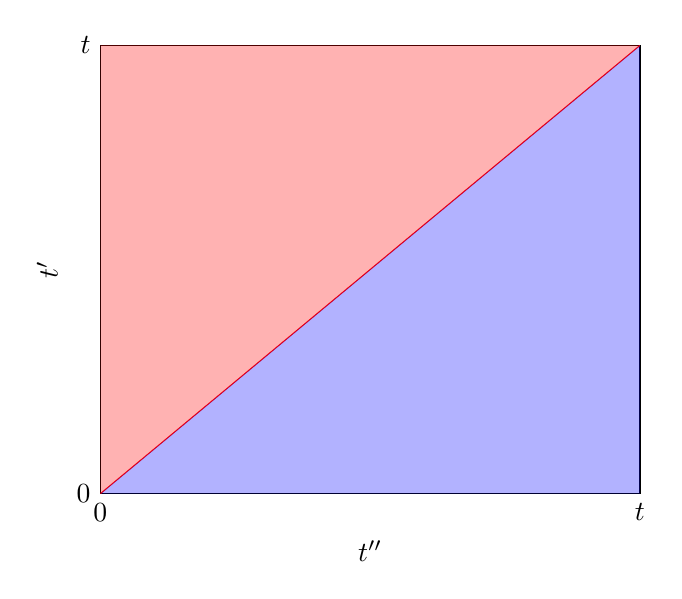
\begin{tikzpicture}
\begin{axis}[
xmin = 0, xmax = 10,
ymin = 0, ymax = 10,
xlabel=$t''$,
ylabel=$t'$,
%yticklabels=\empty,
%xticklabels=\empty,
xtick={0,10}, 
xticklabels={$0$,$t$},
ytick={0,10}, 
yticklabels={$0 $, $ t$} 
]
\addplot[red, domain=0:10] {x};


\begin{scope}
\fill [blue,opacity=.3] (0, 0) -- (100, 100) -- (100, 0);
\fill [red,opacity=.3] (0, 0) -- (100, 100) -- (0, 100); 
\end{scope}
\end{axis}

\end{tikzpicture}
\caption{The integration variables add up to a square!} 
\label{fig:intAdd}
\end{figure}

With this choice of dummy variable our integration variables
are defined so that 
\[
t \ge t' \ge  t'' > t_0 
\] This is shown in the figure \ref{fig:intAdd}. 
So, by the definition of time ordering, in this \textbf{range}, 
we have that 
\[
\int_{ t_0 } ^ t dt' \int_{ t_0 } ^{ t' } dt'' H_{ I } ( t' ) H_{ I } ( t'' ) = \int_{ t_0 } ^ t dt' \int_{ t_0 } ^{ t' } dt'' \mathcal{ T } ( H_{ I } ( t' ) H_{ I } ( t'' ) ) \] However, integration variables are just dummies, so 
we can relabel them. If we relabel $ t' \to t''$, and 
$ t'' \to  t' $, then we have that 
\[
\int_{ t_0 } ^ t dt'' \int_{ t_0 } ^{ t'' } dt' H_{ I } ( t'' ) H_{ I } ( t' )  = \int_{ t_0 } ^ t dt' \int_{ t_0 } ^{ t' } dt'' H_{ I } ( t' ) H_{ I } ( t'' ) 
\] But in this case, our first expression has ranges defined by $ t \geq t'' \geq t' > t_0 $. 
This is the red portion of our square in 
the diagram. 
This is also consistent with time ordering, so we can put our time ordering symbol in the integrand 
so that in this range, $ H_{ I } (t'') H_{ I  }  ( t' ) = \mathcal{ T } ( H _I ( t' ) H _ I ( t'' ) ) $.  
Hence, we can write our second term as 

\[
\int_{ t_0 } ^ t dt' \int_{ t_0 } ^{ t' } dt'' H_{ I } ( t' ) H_{ I } ( t'' ) =\frac{1}{2 } \left(  \int_{ t_ 0 } ^ t dt'' \int_{ t_0 }^{ t''} dt' \mathcal{ T } ( H_{ I }( t' ) H_{ I } ( t'' )  + \int _{ t_0 } ^ t dt' \int_{ t_0  }^{ t' } dt'' \mathcal{ T } ( H_I ( t' ) H _ I ( t'' ) ) \right)  
\] So, we have the same term in the integrand, $ \mathcal{ T } ( H_ I ( t' ) H _ I ( t'') $!
But, the ranges combined on the right hand side of 
this expression is just the full square. 
Hence, we can just integrate over the whole square to get that that
\[
\int_{ t_0 } ^ t dt' \int_{ t_0 } ^{ t' } dt'' H_{ I } ( t' ) H_{ I } ( t'' ) = \frac{1}{2 } \int_{ t_0 } ^ t dt' \int_{ t_0  }^ t dt'' \mathcal{ T } ( H _I ( t' ) H_ I ( t'' ) )  
\]  In full generality, we can expand this 
idea to more integrals and write 
\[
\int_{ t_0  } ^ t dt_1 \int_{ t_ 0 } ^{ t_1 } dt_2 \dots \int_{ t_0 } ^{ t_{ n - 1  } } dt_{ n } H_I ( t_1) \dots  H_{ I } ( t_{ n } )  = \frac{1}{n ! } \int_{ t_0 } ^ t dt_1 \dots \int_{ t_0 } ^{ t  } \mathcal{ T } \left(  H _ I ( t_1 ) \dots H _ I ( t_{ n } )  \right) 
\]  
Thus, we can write 
\[
U ( t, t_0) = 1 + ( -i ) \int_{ t_0 } ^ t dt' H_I ( t' ) + \frac{ ( -i ) ^ 2 }{2 } \int_{ t_0 }^t dt' \int_{ t_0 }^ t dt'' T \left\{  H_I ( t' ) H_I ( t'' )  \right\}  
\] This is Dyson's formula. 
\[
U ( t, t_0) = T \text{ exp } \left\{  - i \int_{ t_0 } ^ t dt' \, H_I ( t' )  \right\} 
\] Alternatively was have that, using the Lagrangian instead, that 
\[
U ( t, t_0 ) = T \exp \left\{  i \int_{ t_0 } ^ t  d^ 3 x dt ' \mathcal{ L }_ I ( t' )  \right\} 
\] For scalar Yukawa theory,  this would be 
\[
T \exp \left\{   - i g \int d^  4 x \psi ^ * \psi \phi  \right\} 
\] This is something of a formal result. 
We expand this to finite order to get some results for scattering
amplitudes which we will derive below in the next section. 

\subsection{ Scattering } 
The time evolution used in scattering theory is called 
the 'S-matrix', where
\[
S= \lim_{t  \to \infty, t_0 \to  - \infty}U ( t, t_0 )   
\] The initial state $ \ket{i } $ and final state $ \ket{ \phi }  $ 
are some sense 'far away' form each other and the interaction. 
We assume that $ \ket{ i } , \ket{ f  } $ behave like free particles; 
they're eigenstates of $ H_0 $ . 
THe amplitude is 
\[
\lim_{ t  \to \infty, t_0 \to  - \infty } \bra{  f} U ( t, t_0 )\ket { i }  = \bra{ f} S \ket{ i }   
\] The latter expression is called the 'S-matrix' matrix element.

\subsubsection{An example with Yukawa theory} 
Going back to scalar Yukawa theory, the interaction Hamiltonian is
\[
H_ I = g \psi _ I ^ * \psi _ I \phi _ I 
\] We model the creation of mesons with $ \phi $, and the creation of nucleons or anti nucleons with $ \psi $. 
Concentrating on the creation and annihilation operators in the 
Fourier mode expansion,
\[
\phi \sim a_{ \vec{p} } + a_{ \vec{p} }^ \dagger 
\] These things destroy and create mesons respectively. 
We have that 
\begin{itemize}
\item $ \psi \sim b_{ \vec{p} } + c_{ \vec{p} }^\dagger $ which destroys a nucleon and create an anti nucleon respectively. 
\item $ \psi ^ *  \sim b_{ \vec{p} } ^ \dagger + c_{ \vec{p} } $ which creates a nucleon and destroys an anti nucleon. 
\end{itemize}
With this interaction, we have the commutation 
relations 
\[
[ a_{ \vec{p} } , a_{ \vec{p} ' }^\dagger ] = [ b_{ \vec{p} }, b_{ \vec{p} ' }^ \dagger ] = [ c_{\vec{p} } , c_{ \vec{p}' }^\dagger ]  = ( 2 \pi ) ^ 3 \delta ( \vec{p} - \vec{p} ' ) 
\] All other commutation relations are zero. 
To our first order our interaction, expanding out 
our interaction Hamiltonian in $ g$, we might have an 
integral term like 
\[
\int dp' dp'' dp'''  b_{\vec{p}}^\dagger c_{\vec{p} ' }^\dagger a_{ }
\] How we we interpret this? 
Well, we could interpret this as a term which destroys 
a meson, then creates a nucleon and anti-nucleon. 

If we expand to second order in $ g$, 
we find more involved terms which stem from our integral. 
For example, we could have the term 
\[
\int ( c^ \dagger b^\dagger a ) ( b c  a^ \dagger ) 
\] This is a two stage process. 
First, from our first bracket term we annihilate a nucleon and an anti-nucleon, 
and then create a scalar meson. 
Then, we annihilate that scalar meson an then create a nucleon and anti-nucleon. 
Thus, this is nucleon and anti-nucleon scattering, and is 
represented by the process
\[
\psi \overline{\psi } \to \phi \to \psi \overline{\psi }
\] Thus, this term \textbf{specifically } contributes 
to nucleon and anti-nucleon scattering. 

\subsubsection{First order term in meson decay}
In this part, we will be focusing on probability 
amplitudes that arise from certain processes. 
Let's focus specifically on the case 
of our first order interaction with a meson  $ \phi $ 
decaying into a nucleon and anti-nucleon
\[
\phi \to \psi \overline{ \psi }
\] Let's give a momentum to our meson, $ \vec{p}$. 
Treating this as an initial state, we assume that 
we can use the ground state of our free theory, $ \ket{ 0 } $, 
as a springboard to excite states from. Thus, we write down 
the momentum eigenstate for our initial state as 
\[
\ket{ i } = \sqrt{ 2E_{ p   } } a_{ \vec{p} }^ \dagger \ket{ 0 }  
\] If we assign our final state $ \ket{ f  } $ to be  
a nucleon and anti nucleon with momenta $ \vec{q}_1,  \vec{q}_ 2 $, 
then we have 
\[
\ket{ f  }  = \sqrt{ 4 E_{ q_1 } E_{ q _ 2 } }  b_{ \vec{q}_ 1 }^ \dagger c_{ \vec{q}_ 2 }^\dagger \ket{ 0 } 
\]  
Our scattering amplitude is given by 
\[\bra{ f } S \ket{ i } = \bra{ 0 } bc a ^ \dagger \ket{ 0 } - ig \bra{ f }  \int d^4 x \, \psi_I^* ( x) \psi_I  ( x) \phi_I ( x) \ket{ 0 }  + O ( g ^ 2 ) \] The zeroth order term is just zero, because $ a^ \dagger , c $ commute. 
Once we commute the $c $ past $ a ^ \dagger $, it hits our vacuum 
state and sends it to zero. 
The form of the first order term deserved some explanation. 
Since we're taking the limit as $ t \to \infty $ and $ t_0 \to  - \infty $, 
the form of our first order term is 
\[
\bra{ f} \int_{ - \infty }^\infty dt \int d^ 3 x \psi^ *_ I  ( x) \psi_ I  ( x) \phi_I  ( x)  \ket{ i } 
\] we can compose the integrals together to get $ \int d^4 x $.
Let's go slowly. We expand on the right hand side our $ \ket{ i } $ term 
to get that 
\begin{align*}
\bra { f} S \ket{ i } & = - i g \bra{f} \int d^ 4 x \, \psi ^ * ( x) \psi ( x) \int \frac{ d^ 3 k }{ ( 2 \pi ) ^ 3  \sqrt{ 2 E_{ k  } }  	 } \left(  a_{ \vec{k} } a_{ \vec{p} } ^ \dagger e ^{  - i k \cdot  x } + a_{ \vec{k} } ^ \dagger a_{ \vec{p} } ^ \dagger e^{ - k \cdot  x } \right) \ket{ 0 }  \\
      & =    \int d^ 4 x \, d^ 3 k  \, \bra{f} \psi ^ * ( x) \psi ( x) \frac{ 1 }{ ( 2 \pi ) ^ 3  \sqrt{ 2 E_{ k  } }  	 } \left(  a_{ \vec{k} } a_{ \vec{p} } ^ \dagger e ^{  - i k \cdot  x } + a_{ \vec{k} } ^ \dagger a_{ \vec{p} } ^ \dagger e^{ - k \cdot  x } \right) \ket{ 0 }
\end{align*} Now, since our $ a_{ \vec{k} } ^ \dagger $ commutes with $ b, c, b ^ \dagger, c^ \dagger $, 
we have that the second term trivially commutes past the $ \psi $ and $ \psi ^ * $ term, and it 
the part goes to zero. As for the first term, 
we commute $ a_{ \vec{k} } $ past and $ a_{ \vec{p} }^ \dagger $, to pick up 
a $ ( 2 \pi ) ^ 3 \delta ( \vec{k} - \vec{p} ) $. 
Thus we replace 
\[
a_{ \vec{k} } a_{ \vec{p}  }^\dagger \ket{ 0 } = [ a_{ \vec{k} }, a_{ \vec{p} } ^ \dagger ] \ket{ 0 }  = ( 2 \pi ) ^ 3 \delta ( \vec{p}  - \vec{k} ) \ket{ 0 }  
\] This means that our term above is 
\begin{align*}
\bra{ f} S \ket{ i } &= - ig \int \frac{ d^ 4 x d^  3 k_1 d^ 3 k_ 2  }{ ( 2 \pi ) ^ 6} \sqrt{ 4 E_{ q_1 } E_{ q_2 }} \bra{ 0 }\frac{1}{ \sqrt{ 4 E_{ k_1 } E_{ k_2 } }} c_{ \vec{q}_2 } b_{ \vec{q}_1 } \left(  b_{\vec{k}_ 1 } ^ \dagger e^{ i k_1 \cdot  x } + c_{ \vec{k}_1 } e^{  - i k_1 \cdot  x } \right) \\
& \left( b_{ \vec{k}_ 2  } e^{ - i k_2 \cdot  x  } + c_{\vec{k}_ 2 }^\dagger e^{ i k_2 \cdot  x } \right) e^{ - i p \cdot  x } \ket{ 0 }  
\end{align*}

We can create a caricature of this product by ignoring the 
momenta and integrals. We get a string of operators 
that look like 
\[
\sim c b b ^\dagger b + c b b ^\dagger c^ \dagger + c  b c b + c b c c^\dagger 
\] Now, all strings ending with $ b $ vanish since they 
operate on the $ \ket{ 0 } $ term to the right. 

We're left with the terms 
\[
\sim c b b ^ \dagger c ^ \dagger + c b c c^ \dagger 
\] Now, in the second term, if we commute $ c $ past  $ c ^ \dagger$, 
we pick up a delta function. But this leaves a term of the form  $ \delta c b $, 
and the  $b  $ still annihilates. So, our only surviving term is 
\[
\sim c b b ^ \dagger c ^ \dagger = c_{ \vec{q} _ 2 } b_{ \vec{q}_ 1 }b_{ \vec{k} _ 1}^\dagger c_{ \vec{k} _ 2 }^\dagger  
\] Commuting $ b $ past $ b^ \dagger$ gives the following term in our integral!
\[
( 2 \pi ) ^ 3 \delta ( \vec{q}_ 1 - \vec{k}_ 1 ) c_{ \vec{q}_ 2 } c_{ \vec{k} _ 2 } ^ \dagger e^{ i x\cdot   ( k_1 + k_2 - p)  }
\] Once again, commuting $ c $ past $ c ^ \dagger $ gives us another delta function to include. 
So the only term preserved in our integral is 
\[
( 2 \pi ) ^ 6  \delta ( \vec{q}_ 1 - \vec{k}_ 1 ) \delta( \vec{q}_ 2 - \vec{k}_ 2 )  e^{ i x\cdot   ( k_1 + k_2 - p }
\] Thus, performing our integrals over $ \vec{k}_ 1 $ and $ \vec{k}_ 2 $ gives us our only term 
at first order which contributes to our scattering. 
\[
\bra{ f} S \ket{ i } =  - i g \bra{ 0 } \int d^ 4 x \, e^{ i ( q_1 + q_2 - p ) \cdot  p } \ket{ 0 }  = - ig \delta ^ 4 ( q_ 1 + q_ 2 - p ) 
\] But, this gives a final amplitude which is a delta function in 4 space. 
This means that for a non zero scattering amplitude, we require our four momentum to be conserved!

\subsection{Wick's theorem} 
\textit{This section follows Prof. B. Allanach's lectures in 2019 as well as 
some of the content on symmetry factors from Peskin and Schroesder.} 

\subsubsection{Why we need Wick's theorem} 

From Dyson's formula, we have 'powers' 
our of our interaction Hamiltonian $ \mathcal{ H }_ I$
that we need to contract with some
set of initial and final states. 
In other words, we wish to compute various quantities in the amplitude calculation, for 
example things like 
\[
\bra{ f } T \left\{  \mathcal{ H } _ I ( x_1) \dots \mathcal{ H }_ I ( x_{ n  })  \right\}\ket{ i }  
\] Calculating this is quite involved, but there's a handy tool that 
we can use to make life easier. If we were able to 
write this in terms of normal ordered products, we could 
instantly take a lot of terms to zero since things that 
are normal ordered have an annihilation operator to the right. 

\subsubsection{An example with scalar fields} 
Let's illustrate how normal ordering can 
make calculations easier principle with the scalar fields
that we have worked with from the Klein-Gordon equation. 
We write out our scalar field as 
\[
\phi ( x ) = \phi ^ + ( x ) + \phi ^ - ( x) 
\] In this convention, we set 
\[
\phi ^ + ( x) = \int \frac{ d^ 3 p }{ ( 2 \pi ) ^ 3 } a_{ \vec{p} } e^{  - i p \cdot  x }, \quad \phi ^ - ( x) = \int \frac{d^ 3 p }{ ( 2 \pi ) ^ 3 } a^\dagger_{ \vec{p} } e ^{ i p \cdot  x }
\] Now, notice that due to the fact that $ \phi ^ +$ and $ \phi ^ - $ each have either a
creation or annihilation operator, we have that 
\[
\phi ^ + ( x) \ket{ 0 } = 0 , \quad \bra{ 0 } \phi ^  -( x)  = 0 
\] Let's compute our time ordered product of two scalar fields, 
but expand in terms of these objects. 
For our time ordered product, we have that for $ x^ 0 > y ^ 0 $
\begin{align*}
T \left\{  \phi ( x) \phi ( y )  \right\}  &=  \phi ( x) \phi ( y )  \\
					   &=  ( \phi ^ + ( x) + \phi ^ - ( x ) ) ( \phi ^ + ( y ) + \phi ^ - ( y ) )  \\
					   &=  \phi ^ + ( x)  \phi ^ + ( y ) + \phi ^ - ( x) \phi ^ + ( y ) + \phi ^ - ( y ) \phi ^ + ( x) + \phi ^ - ( x) \phi ^ - ( y ) + [ \phi ^ + ( x) , \phi ^ - ( y ) ]   
\end{align*} 
We've added in a commutator here for a good reason. 
We've done this to ensure that all the $ \phi ^ - $ terms 
are pushed to the left. Thus, note that our first four terms are normal ordered, 
since contraction with the vacuum state on either 
side will send each of those terms to zero. 
Thus, we can write this as 
\[
T \left\{  \phi ( x) \phi ( y ) \right\} 	= : \phi ( x) \phi ( y ) : + \int \frac{ d^ 3 p d^ 3 p' }{ ( 2 \pi ) ^ 6 \sqrt{ 4 E_{ p } E _{ p '  } }  } [ a_{ \vec{p} } , a_{ \vec{p}' } ] e ^{  - i p \cdot  x  +i p ' \cdot  y } 
\] But the second term is just our expression for the propagator between 
two scalar fields! So we have 
\[
\phi ( x) \phi ( y ) = : \phi ( x) \phi ( y ) : +  D( x - y ) 
\] Similarly, for the case $ y ^ 0 > x ^ 0 $, 
we have that 
\[
 T \left\{  \phi ( x) \phi ( y )  \right\}  = : \phi ( x) \phi ( y ) : + D ( y - x) 
\] If we put these two results together, we find that 
\[
 T \left\{ \phi ( x) \phi ( y )  \right\}  = : \phi ( x) \phi ( y ) : + \Delta_ F( x - y )  
\] Note that our Feynman propagator is just a function.

\pagebreak 
\subsubsection{Contractions and Wick's Theorem}  
We define a contraction on a pair of fields to look like $ \contraction{}{ \phi_1 } { } { \phi _ 2 } \phi_1 \phi_2  $
to replace this pair with the Feynman propagator. 
For example, writing down the string 
\[
 \contraction{\phi( x_1 ) }{ \phi( x_2) }{ \dots }{ \phi ( x_{ j } )  } \phi( x_1 ) \phi ( x_2 ) \dots \phi ( x_{j } ) \dots \phi ( x_{ n }) 
\] to mean replacing the 2 fields with the propagator $ \Delta_F ( x_2 - x_{ j } ) $. 

Thus, in the case of two fields, we have
\[
T \left\{ \phi ( x) \phi ( y )  \right\} = : \phi ( x) \phi ( y ) : + \contraction{}{\phi ( x) } { } { \phi ( y ) }{ } \phi ( x) \phi ( y ) 
\]
Now, we would like to generalise the above principle with $n$ scalar fields, $\psi(x_1),  \psi(x_2), \dots, \psi(x_n) $, to calculate the time ordered product $ \mathcal{T} \psi(x_1) \psi(x_2) \dots \psi(x_n) $. This result is surprisingly elegant. The result is the normalsum of the normal string of the field, along with the normal ordering of \textbf{all} possible contractions. This is Wick's theorem.
\[ 
\mathcal{T} \psi(x_1) \psi(x_2) \dots \psi(x_n) = :\psi(x_1) \dots \psi(x_n): + : \text{terms with all possible contractions}: \] 

It's easy to see that our previous result with two scalar fields agrees with the result. Now, let's examine what happens with three scalar fields. Remember, we add in all possible contractions with normal ordering. For brevity, we will denote $\phi(x_1) = \phi_1$. Thus, we have \begin{align*}  \mathcal{T}( \phi_1 \phi_2 \phi_3 ) &= :\phi_1 \phi_2 \phi_3:
+ :\contraction{}{\phi_1}{\phi_2}{\phi_3} \phi_1 \phi_2 \phi_3: + :\contraction{}{\phi_1}{}{\phi_2} \phi_1 \phi_2 \phi_3: + :\contraction{\phi_1}{\phi_2}{}{\phi_3} \phi_1 \phi_2 \phi_3 :  \end{align*} 
It's important now to realise that a term like $\contraction{}{\phi_1}{}{\phi_2} \phi_1 \phi_2$ is just a number. So, we can 'factor' this out of our normal operator. So, a lot of the terms in the above sum actually look more like \[ :\contraction{\phi_1} {\phi_2 }{}{\phi_3} \phi_1 \phi_2 \phi_3 : = \contraction{}{\phi_2}{}{\phi_3} \phi_2 \phi_3 :\phi_1: \] Now, the important thing here is that since every term has a string of operators which are normal ordered, when we contract on either side with $\ket{0}$, we get zero. Hence, we have that \[ \bra{0}\mathcal{T}(\phi_1 \phi_2 \phi_3)\ket{0} = 0 \] and in general, the time ordered string of an odd number of scalar fields goes to zero.  
Now, let's do the case with four scalar fields: 
\[ T(\phi_1 \phi_2 \phi_3 \phi_4 )  = :\phi_1 \phi_2 \phi_3 \phi_4:  + :\text{terms with 1 contraction}: + : \text{terms with 2 contractions} : \] 
where a term with one contraction might look like \[ :\contraction{}{\phi_1}{\phi_2 \phi_3} {\phi_4} \phi_1 \phi_2 \phi_3 \phi_4 : \] and a term with two contractions might look like\[ :\contraction{}{\phi_1}{}{\phi_2} \phi_1 \phi_2 \contraction{}{\phi_3}{}{\phi_4} \phi_3 \phi_4: \] which in this case is just a complex number, because we've contracted everything out. We can start counting the number of terms in each sum. There are 6 ways to choose two unordered pairs from four objects, so we have six terms in the first sum. There are 3 ways to choose two unordered pairs from four objects, so there are 3 terms in the second sum. 
These terms in the second sum are \[ \contraction{}{\phi_1}{}{\phi_2} \phi_1 \phi_2 \contraction{}{\phi_3}{}{\phi_4}\phi_3\phi_4, \quad \contraction{}{\phi_1}{\phi_2}{\phi_3} \contraction[2ex]{\phi_1}{\phi_2}{\phi_3}{\phi_4} \phi_1\phi_2 \phi_3 \phi_4, \quad \contraction{}{\phi_1}{\phi_2 \phi_3}{\phi_4} \contraction[2ex]{\phi_1}{\phi_2}{}{\phi_3} \phi_1\phi_2 \phi_3 \phi_4 \]
These are the only non zero terms under contraction with $\ket{0}$ on both sides since there are no normal ordered operators here, just complex numbers. Hence, upon contraction we have that only these term survive and our final expression is 
\[ \bra{0}\mathcal{T} \phi_1 \phi_ 2\phi_3 \phi_4 \ket{0} = \Delta_F(x_1 - x_2)\Delta_F(x_1 - x_3) + \Delta_F( x_1 - x_3 ) \Delta_F( x_2 - x_4 ) + \Delta_F( x_1 - x_4 )\Delta_F( x_2 - x_3) \]   

We can visualise these Feynman progagstors diagramatically, by assigning nodes and lines to the propagators involved in the sum. For example, in the two scalar field case, we have our representation as 

\begin{figure}
\centering  
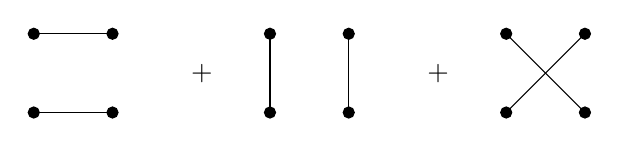
\begin{tikzpicture}
\filldraw[black] (0, 0) circle (2pt);
\filldraw[black] (1, 0) circle (2pt); 
\filldraw[black] (0, -1) circle (2pt);
\filldraw[black] (1, -1) circle (2pt);

\draw (0, 0) -- (1, 0) ;
\draw (0, -1) -- (1, -1);

\filldraw[black] (3, 0) circle (2pt); 
\filldraw[black] (4, 0) circle (2pt); 
\filldraw[black] (3, -1) circle (2pt); 
\filldraw[black] (4, -1) circle (2pt); 

\draw (3, 0) -- ( 3, -1); 
\draw (4, 0) -- (4, -1);

\filldraw[black] (6, 0) circle (2pt); 
\filldraw[black] (7, 0) circle (2pt);
\filldraw[black] (6, -1) circle (2pt); 
\filldraw[black] (7, -1) circle (2pt);

\draw (6, 0 ) -- (7, -1); 
\draw ( 7, 0) -- (6, -1); 

\node[text width=0cm] at (2, -0.5) {+} ; 
\node[text width=0cm] at (5, -0.5) {+} ; 
\end{tikzpicture}
\caption{Diagram corresponding to Wick's theorem with four space time points} 
\end{figure}  
In each of the separate diagrams, the nodes represent the space time points $x_1, x_2, x_3$ and $x_4$. Our early interpretation of this is particle creation at one end of the line at some node $x_j$, and then propagation in space time before annihilation at the other end of the line at node $x_k$. 

For example, for four fields, we have that 
\begin{align*}
T \left\{ \phi_1 \phi_2 \phi_3 \phi_4  \right\} &=  : \phi_1 \phi_2 \phi_3 \phi_4  \\
						& + ( \contraction{}{\phi_1 } { } { \phi_2} \phi _ 1 \phi_2 : \phi_3 \phi_4: + \text{ 4 similar terms } ) \\
						& + \contraction{}{ \phi_1} {}{\phi_2} \phi_1 \phi_2  \contraction{}{ \phi_3} {}{\phi_3} \phi_3 \phi_4 + \text{ 2 similar terms}
\end{align*} 
This is useful because when we sandwich these terms between vacuum states, normal 
ordered terms vanish. Hence,  
\[ \bra{0}\mathcal{T} \phi_1 \phi_ 2\phi_3 \phi_4 \ket{0} = \Delta_F(x_1 - x_2)\Delta_F(x_1 - x_3) + \Delta_F( x_1 - x_3 ) \Delta_F( x_2 - x_4 ) + \Delta_F( x_1 - x_4 )\Delta_F( x_2 - x_3) \]   

The proof of Wick's theorem is by induction , which we already have shown for $ n  = 2 $.
Suppose it's true for  $ T \left\{  \phi_1 \dots \phi_{ n } \right\} $, 
and we left multiply with $ \phi_1 $ with $ \phi_ 1 ^ 0 > \phi_{k } ^ 0 , \forall k \in \left\{  2, \dots n  \right\} $

Then, we have that 
\[
T \left\{ \phi_1 \dots \phi_{ n }  \right\} = ( \phi_1 ^ + \phi_1^ - ) \left[  : \phi_2 \dots \phi _{ n } + : \text{all contractions of } \phi_2 \dots \phi _{ n } :  \right]  
\]  The $ \phi_1 ^ - $ term can stay where it is and go inside the 
normal ordered element since it's in the write place. 
However, the $ \phi_1 ^ + $ term has to be commuted to the RHS 
of all $ \phi_2^ -  \dots \phi_{n } ^ - $, so the RHS can be 
written as normal ordered products. 
Each commutation gives us $ D ( x_1 - x_{ k} ) $, for which 
this time ordering is $ \Delta_F ( x_1 - x_{ k } )  = \contraction{}{\phi_1 } {}{\phi_{ k }} \phi_ 1 \phi _{ k }$. 

\subsubsection{Consequences of Wick's theorem}  
Our first main result which comes from Wick's theorem is that
our time ordered product 
\[
\bra{ 0 } T \left\{ \phi_1 \dots \phi_{ n } \right\} \ket{ 0 } = 0 \quad \text{ if n is odd}
\] This is because, for an odd number of fields,  
fields, no matter how many things we contract we'll 
have at least one thing left over (since we can only contract 
pairs of fields). This means that 
anything contracted with our vacuum states go to zero. 
For even terms, we have that 
\[
\bra{ 0 } T \phi_1 \dots \phi_{ n } \ket{ 0 } = \sum_{ \text{ distinct, symmetric even perms of } \left\{ i_1 , \dots i_{ n } \right\} } \Delta_F( x_{ i_1 } - x_{ i _ 2 }) \Delta_F ( x_{ i _ 3 }  - x _{ i _ 4 } ) \dots \Delta_F( x_{ i _{ n - 1 } } - x_{ i _{ n }} )  
\] We have a graphical representation of this, similar in the case with the 
four scalar fields above. We mark $ x_1, x_2 \dots x_{ n }   $  as points. 
We join pairs of points in all possible ways. Each line corresponds to a propagator for $ \Delta_F$. 

We can apply Wick's theorem to a 
to a $ \mathbb{ C} $ scalar $ \psi $ as well. 

For example, we have that 
\[
T \left\{  \psi ( x) \psi ( y )  \right\}  = : \psi ( x) \psi ^ * ( y ) : + \Delta_F ( x- y ) 
\] Our Feynman propagator now comes from the propagator of 
$ \psi $ and $ \psi ^ * $ with time ordering.  
\[
\contraction{} { \psi ( x) } { } { \psi ^ * ( y )  } \psi ( x) \psi ^ * ( y ) = \Delta_F ( x - y ) 
\] Due to the fact that operators in $ \psi $ and $ \phi $ commute, 
we have that 
\[
\contraction{} { \psi ( x) } { } { \psi  * ( y )  } \psi ( x) \phi  ( y ) = 0 
\] and similarly for $ \psi ^ * ( x) \phi ^ * ( y ) $. 


\subsubsection{Nucleon to Nucleon Scattering} 
Now, let's apply Wick's theorem for nucleon to nucleon scattering with 
\[
\psi ( p_1) \psi ( p_2 ) \to \psi ( p_1' ) \psi ( p_2' ) 
\] We have the initial and final states
\begin{align*}
\ket{ i } & = \sqrt{4 E_{ p_1 } E_{ p_2 }} b_{ \vec{p}_ 1 } ^ \dagger b_{ \vec{p} _ 2 }^\dagger \ket{ 0 }  \\
\ket{ f} &= \sqrt{ 4 E_{ p_1 ' } E_{ p_2 ' } }  b_{ \vec{p}_1 ' } ^ \dagger b_{ \vec{p}_ 2 ' }^ \dagger \ket{ 0 } 
\end{align*}
So far, the only terms of interest to us 
are terms of order $ O ( g )  $ or above. 
We're not interested in processes where no scattering occurs, so 
we look at terms in 
\[
\bra{ f}  ( S - 1) \ket{ i } \quad \text{ at  } O ( g ^ 2)  
\]  The $ -1 $ is there to exclude our case $ \bra { f} \ket { i } $. 
By Dyson's formula, we have that 
\[
\frac{( - i g ) ^ 2 }{ 2 } \int d^ 4 x_1 d^ 4 x_2 \bra{ p_1' , p_2' } T \left\{ \psi^ * ( x_1) \psi ( x_1 ) \phi ( x_1 ) \psi ^ * ( x_2 ) \psi ( x_2 ) \phi ( x_2 )   \right\} \ket { p_1, p_2 }  
\] Using Wick's theorem, 
there's a term in this that looks like 
\[
: \psi ^ * ( x_1 ) \psi ( x_1) \psi ^ * ( x_2 ) \psi ( x_2) : \contraction{ } { \phi ( x_1 ) } { } { \phi ( x_2 ) } \phi ( x_1 ) \phi ( x_2 ) 
\] which will contribute, since the $ \psi $ terms 
will annihilate the initial nucleons and the  $ \psi ^ * $ 
create the final ones. This is the only configuration which 
will give our desired $ \psi \psi \to \psi \psi $ scattering. 
All other terms vanish. Also, observe that if we didn't contract the $ \phi $ terms together 
they would annihilate the vacuum state somehow. Let's call the above contraction $M $.  
\[
\bra{ p_1 ' , p_2 ' }  \psi ^ * ( x_1 ) \psi ( x_1) \psi ^ * ( x_2 ) \psi ( x_2 ) : \ket{ p_1, p_2 }  = M 
\] If we expand out these fields, we
get 
\begin{align*}
\bra { f} ( S - 1 ) \ket { i } = \frac{( - i g )^ 2  }{ 2}\int \frac{ d^ 3 q_1 \dots d^ 3 q_4 }{ \sqrt{ 16 E_{ q_1 } \dots E_{ q_ 4}} } & \frac{ \sqrt{ 16 E_{ p_1 } E_{ p_2 } E_{p_1 ' } E_{ p _ 2 ' }} }{ ( 2 \pi ) ^{ 1 2 }} \bra{ 0 } b_{ \vec{p}_ 1  } '  b _{ \vec{p}_ 2 } ' b_{ \vec{q}_ 1 }^ \dagger b _{ \vec{q}_ 2 } ^ \dagger b_{ \vec{q} _  3} b_{ \vec{q}_ 4 } b _{ \vec{p}_1 } ^ \dagger b _{ \vec{p}_ 2 } ^ \dagger \ket{ 0 } \\
																	& \times e^{ i ( q_1 \cdot  x_1 + q_2 \cdot  x_2 - q_3 \cdot  x_1 - q_4 \cdot  x_2) }
\end{align*} 
For details of Wick's theorem, check out 'Relativistic quantum fields', 
by Bjorkin and drell. 
Using our standard commutation relations, we have that the above expression in 
the brackets is 
\begin{align*}
\bra{ 0 } b_{ \vec{p} _1 ' } b_{ \vec{p}_ 2 ' } b_{\vec{q}_ 1 } ^ \dagger b_{ \vec{q}_ 2 } ^ \dagger b_{ \vec{q} _ 3 } b_{ \vec{q} _ 4 } b_{\vec{p}_ 1 }^ \dagger b_{ \vec{p}_ 2 } ^ \dagger \ket{ 0 } &=  \bra{ 0 } b_{ \vec{p}_ 1 ' } b _{ \vec{p} _ 2 ' } b_{ \vec{q} _ 1 } ^ \dagger b_{ \vec{q} _ 2 } ^ \dagger b_{ \vec{q} _ 3 } 
\left( [ b _{ \vec{q}_ 4 } , b_{ \vec{p}_ 1 } ^ \dagger ] + 
b _{ \vec{p} _ 1} ^ \dagger b _{ \vec{q} _4 } \right) b_{ \vec{p} _ 2 } ^ \dagger \ket{ 0 }  \\
&= \bra{ 0 } b_{ \vec{p} _ 1 '} b_{ \vec{p} _ 2 ' } b_{ \vec{q} _ 1 } ^ \dagger b_{ \vec{q} _ 2 } ^ \dagger
b_{ \vec{q} _ 3 } b_{ \vec{p} _ 2 } ^ \dagger \ket{ 0 } \delta ( \vec{q} _ 4 - \vec{p} _ 1 ) ( 2 \pi ) ^ 3
\\
& + \bra{ 0 } b_{ \vec{p}_ 1 ' } b_{ \vec{p} _ 2 ' } b_{ \vec{q} _ 1 }^ \dagger b_{ \vec{q} _ 2 } ^ \dagger b _{ \vec{q} _ 3 } b_{ \vec{p} _ 1 }^ \dagger [ b_{ \vec{q} _ 4 } , b _{ \vec{p} _ 2 } ^ \dagger]  \ket{ 0 } \\
& = \bra{ 0 } b_{ \vec{p} _ 1 ' } b_{ \vec{p}_ 2 ' } b_{\vec{q} _ 1 } ^ \dagger b_{ \vec{q} _ 2 } ^ \dagger \ket{ 0 } \delta ( \vec{q}_ 3 - \vec{p} _ 2 ) \delta ( \vec{q} _4 - \vec{p}_ 1 ) ( 2 \pi ) ^ 6 \\
&+ \bra{ 0 } b_{\vec{p} _1 '} b_{\vec{p} _ 2 ' } b_{\vec{q} _ 1} ^ \dagger b_{ \vec{q} _ 2 } ^ \dagger \ket{ 0 } ( 2 \pi ) ^ 6 \delta ( \vec{q} _ 4 - \vec{p} _ 2 ) \delta ( \vec{q} _ 3 - \vec{p} _ 1 ) \\
& = \bra{ 0 } b_{ \vec{p} _ 1' } b_{ \vec{p} _ 2 ' } b_{ \vec{q} _ 1 }^ \dagger b_{ \vec{q} _ 2 }^ \dagger \ket{ 0 }  ( 2 \pi ) ^ 6 \left( \delta ( \vec{q} _3 - \vec{p} _ 2 ) \delta ( \vec{q} _ 4 - \vec{p} _ 1 ) + \delta ( \vec{q} _ 4 - \vec{p} _ 2 ) \delta ( \vec{q}_ 3 - \vec{p} _ 1 ) \right) \\
& = 
( 2 \pi ) ^{  12 } \left( \delta ( \vec{p}_ 1 ' - \vec{q} _ 2 ) \delta ( \vec{p}_ 2' - \vec{q} _ 1 )  + \delta ( \vec{p}_2 '  - \vec{q}_ 2 ) \delta ( \vec{p}_1' - \vec{q}_ 1 ) \right) \\
& \times ( \delta ( \vec{q}_ 4 - \vec{p}_ 1 ) \delta ( \vec{q} _ 3 - \vec{p} _ 2 ) + \delta ( \vec{q}_ 4 - \vec{p} _ 2 ) \delta ( \vec{q}_ 3 - \vec{p}_ 1 ) ) 
\end{align*} 


Thus our integrand simplifies to
\begin{align*}
\bra { f } ( S- 1 ) \ket { i } = \frac{ ( - i g ) ^ 2 }{ 2 } \int d^ 4 x_1 d^ 4 x_2 \bigg [ e^{ i x_2 \cdot  ( p_1' - p_1 )  + i x_1 \cdot  ( p_2 ' - p_2 ) } & + 
e^{ i x_2 \cdot  ( p_2' - p_1 ) + i x_1 \cdot  ( p_1' - p_2 ) } + ( x_1 \text{switch with } x_2 ) \bigg ] \\
& \times \int \frac{ d^ 4 k }{ ( 2 \pi ) ^ 4 } \frac{ i e^{ ik \cdot  ( x_2 - x_1 ) }}{k ^ 2 - m ^ 2 + i \epsilon } 
\end{align*}
The switching of $ x_1 $ and $ x_2 $ cancels out 
our factor of $ \frac{1}{2 } $. , since we can 
relabel our $ x_1 $ and $ x_2 $ variables in our 
integration. Thus, we can effectively write our integral as 
\[
\bra{ f} ( S - 1) \ket{ i }  = ( - i g ) ^ 2 \int d ^ 4 x_1 d^ 4 x_2 \left[  e^{ i x_2 \cdot  ( p_1 ' - p_1 ) + i x_1 \cdot  ( p_2 ' - p_2 ) } + e^{ i x_2 \cdot  ( p_2 ' - p_1 ) + i x_1 \cdot  ( p_1 ' - p_2 ) } \right] \int \frac{ d^ 4 k }{ ( 2 \pi ) ^ 4 } \frac{ i e ^{ i k \cdot  ( x_2 - x_1 ) } }{ k ^ 2 - m ^ 2 + i \epsilon } 
\] Note that even though our delta functions 
are over three dimensional space, due to 
the relativistic dispersion relation, our energy component
is determined from just the three momenta. So, our exponents are four vectors
which get pulled out by the three dimensional delta functions. 
Pulling in our integrals over $ x_1 $ and $ x_2 $, 
the above expression is equal to 
\[
\bra { f } ( S- 1 ) \ket { i }  = ( - i g ) ^ 2 \int \frac{ d^ 4 k }{ ( 2 \pi ) ^ 4 } \frac{ i }{ k ^ 2 - m ^ 2 + i \epsilon   } \left[  \delta ( p_1 '  - p_1 + k ) \delta ( p_2 ' - p_2 - k )  + \delta ( p_2' - p_1 + k ) \delta ( p_1' - p_2 - k )  \right]  
\] This finally is 
\[
= ( - i g ) ^ 2 ( 2 \pi ) ^ 4 \left\{  \frac{i }{ ( p_1 - p_1' ) ^ 2 - m ^ 2 + i \epsilon } + \frac{ i}{  ( p_2' - p_1) ^ 2 - m^ 2 + i \epsilon } \right\}
\delta ( p_1 + p_2  - p_1 ' - p_2 ' ) 
\] 

\pagebreak
\subsection{Feynman Diagrams} 
Feynman diagrams are a visual way to represent 
our complicated integrals we've defined above. 
We draw Feynman diagrams to 
represent the expansion of $ \bra { f} ( S - 1) \ket{ i } $ and learn to 
associate functions to them (functions of the four momentum). 
We draw an external line for each particle in $ \ket{ i } $
and $ \ket{ f } $, assigning a four dimensional 
4-momentum to each. We add an arrow for  $ \mathbb{C} $  
fields to show flow of charge. 

The first step is to set up our 
initial and final states. 
We choose an in (out) going arrow in $ \ket{ i } $ for a 
particle (antiparticle), and the opposite for final states $ \bra { f} $. 
These are 'external lines' which don't contribute an integral 
since we're just exciting by an operator like $ b_{ \vec{p} } ^ \dagger \ket{ 0 } $. 

\begin{figure}[htpb]
\centering
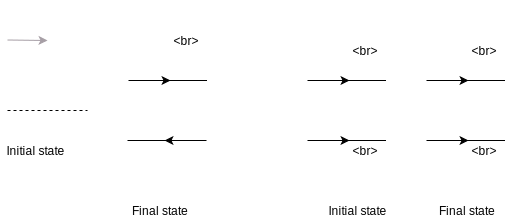
\includegraphics[width=0.8\linewidth]{figures/feyn_1.jpg}
\caption{A template diagram. On the left we have $\phi \to \psi \overline{\psi}$ scattering 
and on the right we have a template for $ \psi \psi \to \psi \psi $ scattering}%
\label{fig:template Feyn}
\end{figure}

We show what kind of diagrams you might have 
for different scattering cases in figure \ref{fig:template Feyn}. 
The next step is to 'fill this in'. We have to be a bit 
careful here. This is is when we need to be aware of what our interaction term looks like. 
For the Yukawa potential, we have our interaction Hamiltonian 
\[
H_I  = \int d^ 3 x \psi ( x) ^ * \psi ( x) \phi ( x) 
\] this means that \textbf{each set of connecting lines} (what we 
call a vertex) in our Feynman diagram needs to look like what we have 
in figure \ref{fig:figures/feyn2}. 
\begin{figure}[htpb]
\centering
\hspace{3cm} \includegraphics[width=0.4\linewidth]{figures/feyn_2.png}
\caption{This is what we must have at each point}%
\label{fig:figures/feyn2}
\end{figure}
We then fill up this diagram with vertices. 
The order of our expansion in $ g $ corresponds 
to how many vertices we have, since each vertex
corresponds to an integral $ \int d^ 4 x H_ I ( x ) $
contributed in Dyson's formula.
Once we've joined together our vertices, we then 
assign a momenta to each line. We have simple examples in the figure. 

\begin{figure}[htpb]
\centering
\includegraphics[width=0.8\linewidth]{figures/feyn_3.png}
\caption{We have some $ O ( g ^ 2 )$ diagrams for $ \psi \psi \to \psi \psi$ scattering}%
\label{fig:figures/feyn_3}
\end{figure}
Our 'internal lines' which are lines with vertices on
both sides are dummy momenta which we integrate over. 
On the other hand, we keep external lines with fixed momenta. 
Each diagram is in 1: 1 correspondence with 
terms in our expansion. 
To each diagram, we evaluate total amplitude using 
Feynman rules for this problem. 
\begin{enumerate}
\item Associate a momentum to each internal line, and keep 
the momenta associated with external legs of the problem 
fixed. 
\item Assign a factor of  $ ( - i g) ( 2 \pi ) ^ 4 \delta ( \sum k_ i ) $
to each vertex, where  $ \sum_i k _ i $ is the sum of 
four momenta flowing \textbf{ in } to the vertex. If momenta 
flows out, this gives a negative momentum contribution. 
\item For each internal line with 4-momenta k, write 
factor 
\[
	\int \frac{ d^ 4 k }{ ( 2 \pi ) ^ 4  } \text{ where } D ( k ^ 2 )  = \begin{cases}
		\frac{ i }{ k ^ 2 - m ^ 2  - i \epsilon } &  \text{ for } \phi \\
		\frac{i }{ k ^ 2 - \mu ^ 2 + i \epsilon } & \text{ for } \psi \\ 
	\end{cases}
\] 
\end{enumerate}
The total amplitude is the sum of all diagrams at the given order. 

\subsection{Scattering revisited} 
Now, to order $ O ( g ^ 2)  $From our first diagram, we have that our contribution is 
given by the sum of the diagrams in figure \ref{fig:figures/feyn_3}. Applying our 
Feynman rules, we have that these diagrams give an integral
of 
\begin{align*}
=( - i g ) ^ 2 \int \frac{ d^ 4 k }{ ( 2 \pi ) ^ 4 } \frac{ i }{ k ^ 2 - m ^ 2 + i \epsilon } &  ( 2 \pi ) ^ 8 ( \delta ( p_1 - p_1 ' - k ) \delta ( p_2 + k - p_2 ' ) \\
										      & + \delta ( p_1 - p_2' - k ) \delta ( p_2 + k - p_1 ' ) ) 	
\end{align*}

Our final scattering momenta to second order 
is therefore 
\[
i (  - i g ) ^ 2 \left\{  \frac{1}{ ( p_1 - p_1 ' ) ^ 2 - m ^ 2 + i \epsilon  } + \frac{1}{ ( p_1 - p_2 ' ) ^ 2 - m ^ 2 + i \epsilon }  \right\} ( 2 \pi ) ^ 4 \delta ( p_1 + p_2 - p_1' - p_2' )  
\] Note that the meson doesn't necessarily satisfy the relation 
that $ k ^ 2 = m ^ 2 $. 
If its doesn't it's called an off shell or virtual particle. 
One might also think that the second diagram in figure 
\ref{fig:figures/feyn_3} is superfluous, but 
we need to count this as a distinct diagram since 
the $ \psi $ are indistinguishable 
under exchange, and hence obey Bose-Einstein statistics
for identical particles.

We can go to even higher order to the point where we 
introduce loops into our diagrams. 


\subsection{Amplitudes} 
In the above, we will always have a factor 
to impose momentum conservation 
between final and initial states. Hence, 
this fact helps us simply things a bit. 
We will define the matrix element $ \mathcal{ M } $ by 
\[
\bra { f} ( S - 1 ) \ket{ i }  = i \mathcal{ M } ( 2 \pi ) ^ 4 \delta ( \sum_{ \text{ final state particles }}  p_i  - \sum_{ \text{ initial state particles }} p_ i ) 
\] Our factor of $ i  $ in our expression 
is done to match conventions with non-relativistic quantum mechanics. 
Our delta function expression follows from translation invariance, and 
is common to all S-matrix elements we compute. 

We now can define a new set of Feynman rules to compute $ i \mathcal{ M  }$, 
which makes things slightly easier. 
\begin{enumerate}
\item We draw all possible diagrams with appropriate external legs, 
and impose 4 momentum conservation at each vertex with appropriate use of delta functions. 
\item We assign a factor of $ ( - ig) $ at each vertex to take into account 
the order of our expansion. 
\item We integrate over closed loops in the diagram, since they give rise
to dummy variables which we can integrate over. So, for closed loops, we 
do the integral $ \int \frac{d^ 4 k }{ ( 2 \pi ) ^ 4 }$. 
\end{enumerate}

We'll now do an example with meson scattering. 

For example, for meson-meson scattering $ \phi \phi \to \phi \phi $, 
we need to draw diagrams. Our lowest order diagram is 
a bit tricky and our requirement that our vertex has to be a 
meson, nucleon and anti-nucleon trio 
means that there'll be a loop. This is shown in figure \ref{fig:mesonLoop}. 

\begin{figure}[htpb]
\centering
\includegraphics[width=0.5\linewidth]{figures/feyn6.png}
\caption{Our lowest order scattering term for $ \phi \phi \to \phi \phi $ decay}%
\label{fig:mesonLoop}
\end{figure}
In the loop, we build up our momentum labels by picking a side as $ k$, 
then just working around whilst using conservation 
of momentum.
This is
\begin{align*} 
\mathcal{ M }  &= \int \frac{ d^ 4 k  }{ ( 2 \pi ) ^ 4  }( - i g ) ^ 4 \frac{i ^ 4 }{ ( k ^ 2 - \mu ^ 2 + i \epsilon ) ( ( k + p_1 ) ^ 2  - \mu ^ 2 + i \epsilon )} \\
	       & \times \frac{1}{( ( k + p_1  - p_1' ) ^ 2 - \mu ^  2+ i \epsilon ) ( k + p_1 ) ^ 2 - \mu ^ 2 + i \epsilon  }
\end{align*} The integrand goes as $ \frac{1}{ k ^ 8 } $, so 
we're sure that this thing converges. 

\pagebreak
\subsection{ Computing the two point correlation function for the ground state of our perturbed Hamiltonian } 
Let's call $\ket {\omega } $ our ground state for our Hamiltonian. A natural question to ask would be what $\bra {\omega } \phi(x) \phi( y ) \ket{\omega} $ is in terms of the spectrum we already know for the free Hamiltonian $H_0$.

One way to do this would be to take the ground state of the free Hamiltonian which we call $\ket{ 0 } $ and expand it in terms of the energy eignestates of the full Hamiltonian. with the full Hamiltonian, the state evolves as \begin{align*} e^{- iHt}\ket{0} &= e^{ - iHt } \ket{\omega}\bra{ \omega }\ket{0} + \sum_{ n \geq 1 }  e^ { -iHt } \ket{n}\bra{n}\ket{ 0 } \\
&= e^ { - iE_0 t } \ket{ \omega }\bra{\omega}\ket{0} + \sum_{n \geq 1} e^{ - i E_n t }\ket{n}\bra{n}\ket{0}   \end{align*}
but by construction we've assigned these energy eignestates in terms of the magnitudes of their energy eigenvectors, so $E_0 < E_1 \dots E_n < \dots $. Thus, to make the terms in the sum disappear, we employ a clever trick. This trick is to basically make the $e^{ - i E_0 t} $ term decay slower than the $e^ { - iE_n t} $ terms, by taking the limit of $t$ to $t \rightarrow (1 - i\epsilon )\infty$, where $\epsilon$ is chosen sufficiently small as to make the terms in the sum decay, but not the exponential term in front of the ground state. Hence our final result is that, our ground state for the full hamiltonian $\ket{\omega} $ can be written as \[ \ket{ \omega} = lim_{t \rightarrow (1  -i \epsilon)\infty  }e^{ - i Ht } \left( e^{ - i E_0 t}\bra{\omega}\ket{0} \right)^{- 1} \]

\subsection{Wick's theorem} 

\subsection{Applying Wick's theorem for the interaction term}
Let's apply Wick's theorem to calculate the next term in the series of our quantity \[ \bra{0} \mathcal{T} \phi(x) \phi(y) \exp \left(  -i  \int dt H_I(t) \right) \ket{0} \] . Let's resume our discussion in the case of $\phi^4$ theory, where our interaction Hamiltonian is $\int d^3 z \phi^4(z) $. Recall, our first term in the series expansion is just \[ \bra{0} \phi(x) \phi(y) \ket{0} = \Delta_F(x -y)  \] and our expression in the series expansion is \[ \bra{0} -i\frac{ \lambda} { 4!}   \mathcal{T} \phi(x) \phi(y)  \int dt \int d^3 z \phi^4 (z) \ket{0} \]       
We can write this a little more concisely by combining writing $\int dt \int d^3z = \int d^4 z$, so we're aware that it's an integral over four space time dimensions. To make it clearer to understand the nature of the contractions in this expression, we do something a bit weird and write out the terms in the $\phi^4$ term as $\phi(z)\phi(z)\phi(z) \phi(z)$. 
We want to cookup a simplified expression for the term \[  - i \frac{ \lambda} {4!} \bra{0}\mathcal{T} \phi(x) \phi(y) \int d^4 z \phi(z) \phi(z) \phi(z) \phi(z) \ket{0} \] Since we have a time ordering operator there, the only non zero terms which surivive once we expand this thing into a sum are the terms where every scalar $\phi$ in contracted with another. The important thing to remember is that this includes the $\phi(z) $ terms incorporated into the integral. There are several contraction we could do here, but the most obvious one to start with is to first contract $\phi(x)$ and $\phi(y)$ together, and then pair up the terms in the integral as follows \[ 
- \frac{ i \lambda} { 4!} \contraction{}{\phi(x) }{} { \phi(y) } \phi(x) \phi(y) \int d^4 z \contraction{}{\phi(z)}{} { \phi(z) } \phi(z) \phi(z) \contraction{}{\phi(z) }{}{\phi(z) } \phi(z) \phi(z) \] but this corresponds to, replacing the contractions with Feynman propagators, \[ - \frac{i \lambda} { 4!} \Delta_F( x - y ) \int d^4 \Delta_F(z - z) \Delta_F(z - z) \] 
Alternatively, we could have contracted the $\phi(z)$ terms differently in the integrand, and instead could have contracted the terms like so: 
\[ - i \frac{ \lambda} { 4!} \contraction{}{\phi(x) }{ } {\phi(y) } \phi(x) \phi(y)  \int d^4 z \contraction{} {\phi(z)}{\phi(z)}{ \phi(z) }  \contraction[2ex]{\phi(z)}{\phi(z)}{\phi(z)}{\phi(z) } \phi(z) \phi(z) \phi(z) \phi(z) \] 
This term here still corresponds to the integral  \[ - \frac{i \lambda} { 4!} \Delta_F( x - y ) \int d^4 z \Delta_F(z - z) \Delta_F(z - z) \]
We count that there are in total 3 different sets of contractions which yield this integral. So the contribution that we have from contractions of this type is  \[ - \frac{3 i \lambda} { 4!} \Delta_F( x - y ) \int d^4 z  \Delta_F(z - z) \Delta_F(z - z) \]   
We represent this type of contraction diagramatically like before in the following diagram.

\begin{figure}[!h] 
\centering
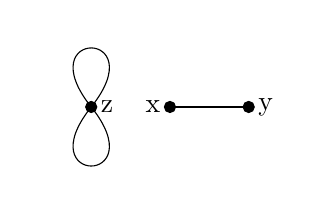
\begin{tikzpicture}
\filldraw[black] (0, 0) circle (2pt) node[anchor=west] {z} ; 
\draw (0, 0) .. controls (0.8, 1) and (-0.8, 1) .. (0, 0);
\draw (0, 0) .. controls (0.8, -1) and (-0.8, -1) .. (0, 0); 

\filldraw[black] (1, 0) circle (2pt) node[anchor=east] {x} ; 
\filldraw[black] (2, 0) circle (2pt) node[anchor=west] {y} ; 
\draw (1, 0) -- (2, 0) ; 
\end{tikzpicture}  
\end{figure} 

We also have another type of contraction that we can include. We contract $\phi(x)$ with one of the $\phi(z)$, and contract $\phi(y) $ with another one. This gives us $12$ choices for our contraction. One of these may look like \[  - \frac{i \lambda}{ 4!} \contraction[2ex]{}{\phi(x) } {\phi(y) \int d^4 z \, }{ \phi(z) } \contraction[3ex]{ \phi(x) } { \phi(y) } { \int d^4 z \, phi(z ) }{\phi(z)} \phi(x) \phi(y ) \int d^4 z \, \phi(z) \phi(z) \contraction{}{\phi(z)} {} {\phi(z)} \phi(z) \phi(z)  \] we count 12 of these, and represent this diagramatically in the figure adjacent.  
\begin{figure}[!h] 
\centering
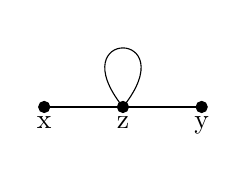
\begin{tikzpicture}
\filldraw[black] (0, 0) circle (2pt) node[anchor=north] {x}; 
\filldraw[black] (1, 0) circle (2pt) node[anchor=north] {z}; 
\filldraw[black] (2, 0) circle (2pt) node[anchor=north] {y}; 

\draw (0, 0) -- (1, 0); 
\draw (1, 0) -- (2, 0); 

\draw (1, 0) .. controls (0.2, 1) and (1.8, 1) .. (1, 0) ; 
\end{tikzpicture}
\end{figure} 
Our total first order contribution is therefore \[ - \frac{ 3i\lambda }{ 4!} D_F(x - y )  \int d^4 z \, D_F(z - z)  D_F(z - z) - \frac{12 i \lambda}{ 4! } \int d^4 z \, D_F( x - z) D_F( y - z) D_F( z - z ) \] which exhausts all of the possible ways to contract terms in our sum above. 

\subsubsection{Symmetry factors} 
We now present a convinient way to find the coefficent of our contribution which a diagram contributes. This is called the symmetry factor of the diagram. It is as follows. Given a particular diagram, 
\begin{enumerate} 
\item Ascribe a symmetry factor of 2 for edges which loop to the same node. 
\item Ascribe a symmetry factor of $n$ for edges which can be interchanged
\item Ascribe a symmetry factor of 2 for vertices which are equivalent. 
\end{enumerate}
As an example, consider the diagram below. 

\pagebreak
\section{The Dirac Equation}

\subsection{What does the Dirac equation give us?} 
The Dirac equation is important because it provides the framework for quantization of spin-$\frac{1}{ 2}$ particles, like electrons and other fermions. Another startling prediction that the Dirac equation gives us is the existence of anti-matter. This equation is an amazing combination of the geometry of spinors in Minkowski space-time, and the wave-function formalisation of quantum mechanics that we all know and love. 
In this section, we'll provide some motivation for constructing the Dirac equation, solve it, then quantise this object to give rise to particles (fermions). 

\subsection{Warming up with spinors from the $SO(3)$ rotation group} 

Spinors are (complex) elements in a vector field which transform linearly when the underlying coordinate basis is rotated. In three dimensional Euclidean space, this transformation would take the form of an element in $SO(3)$, acting on three dimensional real vectors in $\mathbb{R}^3$. Our goal of this subsection is to build an equivalence between this and elements in $SU(2)$, where then these elements act on 2 component complex vectors in $\mathbb{C}^2$.

\subsubsection{Rotations in Euclidean space} 
Let's revise quickly how to map rotations out in three dimensional space. We multiply a vector $\mathbf{v} $ by a matrix to give the map $\mathbf{v} \mapsto R \mathbf{v}$. In the case of a rotation by an angle $\theta$ about the z-axis, our rotation matrix $R_z$ takes the form \[ R_z = \begin{pmatrix} \cos \theta & \sin \theta \\  - \sin \theta & \cos \theta \end{pmatrix} \] 
In the terminology of Lie groups, this is an element of the Lie group $SO(3)$, and has an associated generator $J_z$, given by it's derivative at $\theta = 0$; 
\[ J_z = \left. \frac{d}{ d\theta } R_z (\theta) \right\vert_{ \theta = 0 }  = \begin{pmatrix} 0 & 1 & 0 \\ -1 & 0 & 0 \\ 0 & 0 & 0 \end{pmatrix}  \]
We can repeat this same procedure with rotations along the y and x axes, and differentiate with respect to the parameters as well to obtain the generators $ J_x $ and $J_y$. One finds that these rotation generators obey the following commutation relations, or 'algebra' \[ [ J_i , J_j ] = i \epsilon_{ ijk} J_k \] 

We can then write out a full transformation, which is a rotation by an angle $\theta$ about the normal vector $\mathbf{ n } $, as \[ \mathbf{ v} \mapsto e^{ i  \mathbf{n} \cdot \mathbf{J} \theta } \mathbf{ v} \] where the exponent is simply the expected series sum of the matrices.  

\subsubsection{Transformations with Unitary matrices} 
We now explore the group $SU(2)$, the group of 2 by 2 matrices which satisfy the relation $U^\dagger = U^ { -1} $, and $\det U = 1$. One can show, that by comparing coefficients, that unitary matrices can be written in general of the form 
\[ 
U = \begin{pmatrix} a & b \\  -b^* & a^* \end{pmatrix} 
\] 
where we have the condition that $|a|^2 + |b|^2 = 1 $. Recall that $a$ and $b$ are complex, so over the reals are specified by 2 parameters each. Our condition that $|a|^2 + |b|^2 = 1$ reduces our degrees of freedom by 1, so we have 3 degrees of freedom in total.  
We would like to see how unitary matrices transform vectors of the form \[ \xi = \begin{pmatrix} \xi_1 \\ \xi_2 \end{pmatrix} \]
We have that \[ \xi \mapsto \xi' = U \xi = \begin{pmatrix} 
a \xi_1 + b \xi_2 \\ \ - b^* \xi_1 + a^* \xi_2 \end{pmatrix} = \begin{pmatrix} \xi_1' \\ \xi_2' \end{pmatrix}  \]
Now we ask the question of whether we can find other vectors derived from this which can transform in the same way. Turns out, the vector $( - \xi_2^*, \xi_1^* ) $ does as well. You can verify this yourself! We employ the notation that Ryder uses here, using the sign $\sim $ to denote 'transforms as', we've discovered that \[ (\xi_1, \xi_2) \sim (  -\xi_2^*, \xi_1^* ) \] 
Or, setting \[ \chi = \begin{pmatrix} 0 & -1 \\  1 & 0 \end{pmatrix} \] we can alternatively write that $ \xi \sim \chi \xi^* $. Now, this also means that, taking the hermitian conjugate of a vector, that $\xi^\dagger $ transforms as $ ( - \xi_2 , \xi_1 ) $ 
which implies that $\xi \xi^\dagger$ transforms as \[ 
H = \begin{pmatrix} \xi_1 \\ \xi_2 \end{pmatrix} ( -\xi_2, \xi_1) = 
\begin{pmatrix}  - \xi_1 \xi_2 & \xi_1^2 \\  - \xi_2^2 & \xi_1 \xi_2 \end{pmatrix} \] 
But we already know that since we have the transformation laws $\xi \mapsto U \xi$ and $\xi^\dagger \mapsto \xi U^\dagger$, \[ 
\xi \xi^\dagger \mapsto U \xi \xi^\dagger U^\dagger \implies H \mapsto U H U^\dagger  = U H U^{ -1 }  \]
The main reason why we've invested so much into finding this matrix which transforms under $U$ is that $H$ is indeed traceless. So, we can write out a matrix which transforms under $U$ in the way we want by giving ourselves a complex traceless matrix, which we'll call $h$. Now, $h$ can be written as \[ h = \begin{pmatrix} z & x + iy \\ x - iy & - z  \end{pmatrix} = \mathbf {\sigma} \cdot \mathbf{x}  \] where $\mathbf{ x} $ is our original position vector we've rotated, and $\mathbf{\sigma} $ are the Pauli sigma matrices. So, we've taken a vector rotating in $SO ( 3) $ and have reduced it down to induced rotations by $SU(2) $. By contruction we've shown that $h \mapsto UhU^{ -1}$, and so we've shown that unitary transformations acting on spinors in $SU(2)$ correspond to rotations acting on position vectors in $SO ( 3) $. We have a specifc map from the spinors to the position vector, given by comparing elements of $h$ and $H$
\[ x = \frac{1}{ 2} ( \xi_1+ \xi_2), \quad y = \frac{ 1}{ 2i } (\xi_1^2 + \xi_2^2 ), \quad z = \xi_1 \xi_2 \] 


\subsection{Lorentz tranformations and spinors}  
To motivate the derivation of the Dirac equation, we need to first discuss in general, objects which transform sensibly with Lorentz transformations. If we have a coordinate system denoted by $x^\mu$, we Lorentz transform it with the map $x^\mu \rightarrow \Lambda\indices{^\mu_\nu} x^\nu$. If we had a scalar field $\psi(x)$, then this passive transformation would induce the transformation \[ 
\psi(x) \rightarrow \psi(\Lambda^{ -1} x) \] 
Now, instead of a scalar field, we might wish to consider what happens to, say, a vector field when we induce a Lorentz transformation. In the case that our vector field transforms linearly in response to Lorentz transformations, we have a spinor. More specifically, we have a complex vector field $\psi^a (x) $ which obeys the transformation law 
\[ \psi^a (x) \rightarrow \Lambda\indices{^a_b}\psi^b(x ) \] 


Suppose we had some eaution which a scalar field $\phi$ satisfies. For example, we have the Klein-Gordon equation 
\[ \left( \partial_\mu\partial^\mu - m^2 \right) \phi = 0 \]. If we were to perform a Lorentz boost which shifts our frame of reference, then it only makes physical sense that the equation still holds, because nothing about the actual physical system has changed. Suppose that our Lorentz boost is written as 
\[ x^\mu \rightarrow x'^\mu  = \Lambda\indices{^\mu_\nu}x^\nu \]
Then our corresponding scalar field should transform as 
\[ \phi(x) \rightarrow \phi(\Lambda^{-1} x) \] 
We can chack that, under this transformation, the Klein-Gordon equation still holds. 


We can generalise this kind of transformation to a field with multiple components which we index as $\phi_a(x) $. As inspiration, we explore how some vector field $V^i$ in three dimensions transforms under a rotation.
\[ 
V^i \rightarrow V'^i  = R^{ij}V^j 
\]
and so we'd expect a Lorentz boost to have a scalar field transform like 
\[
\phi_a(x) \rightarrow \phi'(x)_a = M(\Lambda)\indices{^b_a}\phi_b(\Lambda^{-1}x)
\] 
In the above, we're representing the Lorentz transformation as a matrix $M(\Lambda)$. We call this a representation of our Lorentz transformation. Representations should obey the rule that 
\[ M(\Lambda)M(\Lambda') = M(\Lambda \Lambda')\] or in other words the representation should respect the group structure of Lorentz transformations. Proverbially, we are taking a methematical 'encoding' of our transformation. How do we go about finding the representation $M$? 

Again, we seek inspiration from rotation groups in 3 dimensions. A rotation in 3 dimensions is represented in real space by the matrices in $SO(3)$, which is isomorphic to $SU(2)$. This $SU(2)$ has a basis, which are the Pauli matrices $\sigma_i$. Given a quantum state $\ket{\psi}$, how do we represent its transformation?

Let $\ket{\psi}$ be a wavefunction representing a $\frac{1}{2}$ spin particle. Then, we can represent rotations with thefollowing transformation \[ \ket{\psi} \rightarrow \ket{\psi '}  = \exp{i \mathbf{n} \cdot \mathbf{J}} \ket{\psi} \]
In this case, $J_i$ are the generators of this transformation. We say that the Lie group of rotations in three dimensions are generated by a Lie algebra with commutation relations 
\[ J_k  = i \epsilon_{ijk} [J_i, J_j] \]   
In three dimensions for our rotation group, this operator is given by 
\[ \mathbf{J}  = \mathbf{x} \times \mathbf{p} = \mathbf{x} \times ( - i \nabla) \] 
Where we can index this angular momentum object as 
\[ J^{\nu \mu} = i (x^{\nu} \partial^\mu  - x^\mu \partial^nu) \]
This will precisely be our generalisation for our generatorfor our Lorentz group, except now the indices $\mu, \nu$ are taken over $\mu, \nu = 0, 1, 2, 3$. This object obeys the Lorentz algebra.
\[ [J^{\mu \nu}, J^{\rho \sigma}] = i( - g^{\mu \rho} J^{\nu \sigma} + g^{\mu \sigma}J^{\nu \rho}  - g^{\nu \sigma}J^{\mu \rho} + g^{\nu \rho}J^{\mu \sigma}) \]
And in general, any expression for $J^{\mu \nu}$ which satisfies this equation is a valid representation of our Lie algebra. We denote the components of $J^{\mu \nu}$ by writing down the object with two additional indices $\alpha \beta$. Thus we denote our object by $(J^{\mu \nu})_{\alpha_beta}$. A simple representation that we pull out of the hat is \[ (J^{\mu \nu})_{\alpha \beta} = i \left( \delta\indices{^\mu_\alpha} \delta\indices{^\nu_\beta}  - \delta\indices{^\mu_\beta}\delta\indices{^\nu_\alpha} \right) \] 

Why is this choice intuitive? Well, our Lorentz transformation is obtained by exponentiating our generator that we have here. Thus, for an anti-symmetric 2nd rank tensor, our full transformation is given by 
\[ 
\exp(i \frac{\omega_{\mu \nu}}{2} J^{\mu \nu})
\]
and infinitesimally applied to a 4-vector, our transformation is \[ V^\mu \rightarrow \left( \delta\indices{^\mu_\nu} - \frac{i}{2} \omega_{\alpha\beta}(J^{\alpha\beta})\indices{^\mu_\nu} \right) V^\mu \]

\subsection{Constructing the Chiral representation for the Dirac equation}
You can show that if we have a set of matrices $\{ \gamma^\mu \}_\mu$ which obey the identity 
\[ \{ \gamma^\mu , \gamma^\nu \} =  - 2 g^{\mu\nu}  \] then the object 
\[ S^{ \mu \nu } = \frac{i}{4} [\gamma^\mu, \gamma^\nu] \] obeys the Lorentz algebra which we derived above.  

Whilst this choice of representation is not unique, we choose a canonical one called the Weyl representation which is given by
\[ \gamma^0 = \begin{pmatrix} 0  & I \\ I & 0 \end{pmatrix} \quad \gamma^i = \begin{pmatrix} 0 & \sigma^{i} \\ - \sigma^i & 0 \end{pmatrix} \]  
I'll touch on this a bit more later, but the important this is that this object represents boosts in 3 different dimensions, given by $S^{0i}$ and rotations in 3 dimensions given by $S^{ij}$. 
Thus, our field $\phi(x)$ transforms as, when we exponentiate $S_{ij}$, as \[ \phi(x) \rightarrow \phi'(x) = \exp(i \frac{\omega_{\mu\nu}}{2} S^{\mu\nu}) \phi(\Lambda^{-1}) \] where we've done and inverse transform to represent our change in frame of reference, and also done a map on the field itself.  

\subsection{Motivating Lorentz invariance of the Dirac equation}
In this section, we'll present the Dirac equation and show that it's Lorentz invariant. The way to do this is slightly more convoluted than showing the Lorentz invariance of the Klein-Gordon equation, like we did in the previous section. It involves exploring how $\gamma^\mu$ transforms under both the $S_{ \mu \nu } $ and $ J_{ \mu \nu} $ representations of the Lorentz transformations, and how these representations relate to one another. 

But first, we present the Dirac equation. A field $\psi(x)$ satisfying the Dirac equation satisfies the equation \[ ( i \gamma_\mu \partial^\mu  - m ) \psi( x) = 0  \]
Note that, as opposed to the Klein-Gordon equation, we have a $m$ as the constant term instead of $m^2$. Also notice the fact that we're not taking two derivatives in this equation, we instead contract the derivative $\partial^\mu$ with $\gamma_\mu$. Now, under the Lorentz transformation where $x^\mu \rightarrow x^\nu \Lambda\indices{^\mu_\nu} $, recall our field transforms as \[ 
\psi(x)  \mapsto \Lambda_{ \frac{ 1 }{2 }} \psi( \Lambda^{ -1} x ) \] 
To show that the Dirac equation is invariant under this specific transformation, we require that (for reasons we will show later) \[ 
\Lambda_{ \frac{ 1}{ 2}}^{ -1} \gamma^\mu \Lambda_{ \frac{ 1}{2}}  = \Lambda\indices{ ^\mu_\nu } \gamma^\nu \] 
One can see that if this condition is satisfied, then, upon transforming the equation
\begin{align*} 
( i \gamma^\mu \partial_\mu  -m) \psi & \rightarrow ( i \gamma^\mu \partial_\mu  - m) \Lambda_{ \frac{ 1}{2} } ( \phi \Lambda^{ -1} x )  \\ 
& = \Lambda_{ \frac{1}{ 2} } \Lambda_{ \frac{1}{2} }^{ -1}  ( i \gamma^\mu ( \Lambda^{-1 })\indices{_\mu^\nu} \partial_\nu  - m ) \Lambda_{ \frac{ 1}{2} } \psi( \Lambda^{-1} x ) \\ 
& = \Lambda_{ \frac{ 1}{ 2} } ( i \Lambda_{ \frac{ 1}{2}}^{ -1} \gamma^\mu \Lambda_{ \frac{ 1}{2} } ( \Lambda^{ -1} )\indices{_\mu^\nu} \partial_\nu - m ) \psi( \Lambda^{ -1} x) \\
&= \Lambda_{ \frac{ 1}{2}} ( i \gamma^\mu \partial_\mu  -m ) \psi( \Lambda^{-1} x)    \\ 
&= 0  
\end{align*} 
Let's review carefully what we've done here. In the first line, we've transformed $\psi( x) $ appropriately according to our Lorentz transformation. In the second line, we've done two things. First, we multiply on the left by $\Lambda_{ \frac{1}{2}} \Lambda_{\frac{1}{2}}^{ -1} $ since it's just the identity. In addition, we also pull out a factor of $\Lambda^{-1} $ due to the chain rule. Now, in the third line, we used the identity we've derived above to switch out our expression for $\Lambda_{ \frac{ 1}{2}}^{ -1}  \gamma^\mu \Lambda_{ \frac{1}{2} } $ with just $\Lambda \gamma^\nu $. In doing this, the factors of $\Lambda $ have cancelled each other out. 
The final expression is zero, which means that we've successfully shown that the Dirac equation is Lorentz invariant. 

Now, we'll prove the expression above, by using the infinitesimal generators instead. Observe that the above condition is equivalent to \[ 
( 1 + \frac{ i \omega_{ \rho \sigma} }{ 2} S^{ \rho \sigma} ) \gamma^\mu (1 - \frac{ i \omega_{ \rho \sigma }}{ 2} S^{ \rho \sigma} = ( 1 - \frac{ i \omega_{ \rho \sigma}}{ 2} ( J^{ \rho \sigma} )\indices{ _\mu^\nu}\gamma_nu \] So in turn, if we can show that \[ [\gamma^\mu, S^{\rho \sigma}] = \gamma^\nu (J^{\rho \sigma})\indices{^\mu_\nu} \] we've proven the identity above. We do this as follows 
\[ (J^{\mu \nu} )\indices{_\alpha_\beta}  = i \left( \delta\indices{^\mu_\alpha} \delta\indices{^\nu_\beta} - \delta\indices{^\mu_\beta}\delta\indices{^\nu_\alpha} \right)\]  
When we raise the index on a delta function, we get our metric back. So our expression is 
\[ (J^{\mu\nu})\indices{_\alpha^\beta} = i \left( \delta\indices{^\mu_\alpha} g^{\nu\beta} - g^{\mu\beta}\delta\indices{^\nu_\alpha} \right) \]
Thus \[ \gamma^\alpha (J^{\mu\nu} )\indices{_\alpha^\beta} = i \left( \gamma^\mu g^{\nu\beta} - \gamma^\nu g^{\mu\beta} \right) \]


As for the left hand side \begin{align*} [\gamma^\beta, S^{\mu\nu}] &= [\gamma^\beta, \frac{i}{4} [\gamma^\mu, \gamma^\nu]] \\ &= \frac{i}{4}\left( \gamma^\beta \gamma^\mu \gamma^\nu - \gamma^\beta \gamma^\nu \gamma^\mu - \gamma^\mu \gamma^\nu \gamma^\beta + \gamma^\nu \gamma^\mu \gamma^\beta \right) \end{align*} but we can use the identity that \[ \{ \gamma^\mu , \gamma^\nu \} = - g^{\mu\nu} \] and commute index pairs which are either $( \nu, \beta) $ or $ ( \mu, \beta ) $, to give 
\[ \frac{i} { 4} \left( - \gamma^\mu \gamma^\beta \gamma^\nu - 2g^{\mu \beta } \gamma^\nu  + \gamma^\nu \gamma^\beta \gamma^\mu + 2 g^{\beta \nu} \gamma^\mu + \gamma^\mu \gamma^\beta\gamma^\nu + 2 g^{ \nu \ beta } \gamma^\mu - \gamma^\nu \gamma^\beta \gamma^\mu - 2 \gamma^\nu g^{\mu \beta} \right) \] 
but the terms above cancel to give the correct expression. Hence we've proven the identity above, and have shown that Dirac's equation is Lorentz invariant.  

So we've done all this work - but let's remind ourselves what it's for. This commutation relation is important because it gives us an equation relating the generators $J^{\mu\nu}$ and $S^{ \mu \nu } $. This commutation relation is equivalent to saying, with $\omega_{\rho \sigma} $ as a parameter, that infinitesimally we have \[ \left(  1 + \frac{ i \omega_{ \rho \sigma } S^{ \rho \sigma} }{ 2} \right) \gamma^\mu \left( 1 - \frac{ i \omega_{ \rho\sigma} S^{ \rho \sigma }}{2} \right)  = ( 1 - i ( J^{ \rho \sigma } )\indices{^\mu_\nu})  \gamma^\nu \implies \Lambda_{ \frac{1}{2}}^{ -1} \gamma^\mu \Lambda_{ \frac{1}{2}}  = \Lambda\indices{^\mu_\nu}\gamma^\nu \]  
And with this identity, we've shown that the Dirac equation is Lorentz invariant. 

\subsection{Constructing boosts and rotations in block diagonal form} 
This spinor representation is reducible, which means that we can write out our transformations in block diagonal form. For example, we write out the components of $S^{ \mu \nu } $ explicitly in terms of boosts and rotations, and discover that both the boost and rotations are parametrised by three parameters ( hence we can encode them as vectors). In the boost case, we have that \[ S^{ 0i } = \frac{ i }{2} \begin{pmatrix} 0 & I \\ I & 0 \end{pmatrix} \begin{pmatrix} 0 & \sigma \\ - \sigma_i & 0 \end{pmatrix}  = \frac{i}{2} \begin{pmatrix} - \sigma_i & 0 \\ 0 & \sigma_i \end{pmatrix} \] But, as a tranformation, contracting with $ \omega_{ \mu \nu} $, we're only summing to get $\exp ( \frac{i }{2} \omega_{ 0i }S^{ 0i } )$, and so reparametrising $\omega_{ 0i } = \alpha_i$, we find that our transformation takes the form 
\[ \Lambda_{ \frac{1}{2}}  = \exp \left(i \frac{ \omega_{ \mu \nu} S^{\mu \nu}}{2} \right)  = \begin{pmatrix} e^{ \alpha \cdot \frac{ \sigma}{2} } & 0 \\ 0 & e^{  - \alpha \cdot \frac{\sigma}{2}} \end{pmatrix} \] 
Bear in mind that since we're summing over all the indices, we have an extra factor of $2$. Now, notice that we have a switch in sign under boosts.   

Now we explore what happens when we transform under rotations. Rotations are represented by $S^{ij} $, where $i, j = 0, 1, 2, 3$. Let's compute these matrix representations explicitly - this is also good revision for remembering our Pauli Sigma matrix commutation relations. We have that 
\begin{align*} 
S^{ij}  & = \frac{ i}{4} [\gamma^i, \gamma^j ] \\ 
& = \frac{ i}{ 2} \gamma^i \gamma^j \\
& = \frac{ i}{2} \begin{pmatrix} 0 & \sigma_i \\ - \sigma_i & 0 \end{pmatrix} \begin{pmatrix} 0 & \sigma_j \\ - \sigma_j & 0 \end{pmatrix} \\ 
&= \frac{i}{2} \begin{pmatrix}  - \sigma_i \sigma_j & 0 \\ 0 &  - \sigma_i  \sigma_j \end{pmatrix} 
\end{align*} 

Now, we make use of our Pauli-sigma relations to simplify this expression. One can easily verify that \[ \sigma_i \sigma_j = i \epsilon_{ ijk} \sigma_k  \implies S^{ ij } = \frac{1}{ 2} \epsilon_{ ijk} \begin{pmatrix} \sigma_k & 0 \\ 0 & \sigma_k \end{pmatrix} \]
Now, when we want to contract $S^{ ij }$ with $\omega_{ ij } $ we have that 
\[ 
\omega_{ ij} S^{ ij } = \frac{1}{ 2} \epsilon_{ ijk } \omega_{ ij} \begin{pmatrix} \sigma_k & 0 \\ 0 & \sigma_k \end{pmatrix} \]
But the cool thing abou this is that we can write $\beta_k = \epsilon_{ ijk} \omega_{ij }  $, which gives us the final result for a rotatation transformation, which is 
\[ \Lambda_{\frac{ 1}{ 2} }  = \begin{pmatrix}  \exp^{ - \frac{i}{2} \sigma \cdot \beta } & 0 \\ 0 & \exp^{ - \frac{ i}{ 2} \sigma \cdot \beta } \end{pmatrix} \] 
Where we have a noticable difference with respect to boosts in that there's no sign change between the block diagonal matrices. The fact that we've broken down this spinor representation of Lorentz transformations into two block diagonal matrices is super useful because now we can also split up the spinor vector $ \psi $ into two parts, which we call the left and right handed parts of our spinor. 
\[ \psi = \begin{pmatrix} \psi_L \\ \psi_R \end{pmatrix} \] 
So infinitesimally, we have that \begin{align*} 
\psi_L & \mapsto \left( 1 + \alpha \cdot \frac{ \sigma}{2}  - i  \beta \cdot \frac{\sigma}{2} \right)  \psi_L \\ 
\psi_R & \mapsto \left(  1  -  \alpha \cdot \frac{\sigma}{2}  - i \beta \cdot \frac{\sigma}{ 2} \right)  \psi_R 
\end{align*} 

\subsection{The Weyl equations} 
Let's go back to our Dirac equation, but this time let's view it in the context of our spinor which we split up. We have that \[ 
\left( i \gamma^0 \partial_0 - \gamma^i \partial_i - m  \right) \psi  = 0 \] 

Now, we can write this in the form of a matrix equation, bearing in mind that $m$ acts as a scalar multiple of the identity. Thus, we have the matrix equation \[ 
\begin{pmatrix} 
-m & i (\partial_0 + \sigma \cdot \nabla ) \\
i(\partial_0 - \sigma \cdot \nabla) & -m 
\end{pmatrix} 
\begin{pmatrix} 
\psi_L \\ \psi_R \end{pmatrix} = 0 
\]
In this case, we've mixed the components $\psi_R$ and $\psi_L $. However, we can separate out the mixing by exploring the massless case with $m = 0$, which reduces us to the equations 
\begin{align*}  
( \partial_0 + \sigma \cdot \nabla ) \psi_R & = 0 \\ 
( \partial_0 - \sigma \cdot \nabla ) \psi_L & = 0 
\end{align*} 
We can simplify this notation even further by 'extending' out $\sigma$, and defining the objects 
\[ \sigma^\mu = (1, \sigma ), \quad \bar{ \sigma}^\mu = ( 1,  - \sigma ) \] 
Which gives us a condensed form of the equations to read \begin{align*}  
\sigma^\mu \partial_\mu \psi_R & = 0 \\
\bar{\sigma}^\mu \partial_\mu \psi_L & = 0 
\end{align*} 

\subsection{Constructing Plane-Wave solutions to the Weyl equation} 
At it's essence, the Dirac equation is a wave equation. In this section, we'll explore solutions of Dirac's equation which have the form $\psi(p )  = e^{ - i p x } u ( p ) $, where $p$ denotes momentum, and we have the relativistic dispersion relation where $p^\mu p_\mu = m^2 $. We can make our life easier by reducing the problem to that of the rest frame, where $p^\mu  = (E_\mathbf{p} , 0 ) $. Our dispersion relation then tells us that $p^\mu = (m,  0 )$. Our Dirac equation in matrix form then reads \[ 
\begin{pmatrix}  - m & i ( \partial_0  + \sigma \cdot \nabla ) \\ 
i ( \partial_0  - \sigma \cdot \nabla ) & -m 
\end{pmatrix} e^{ - i p \cdot x } u(  p )  = \begin{pmatrix} -m & m \\ m & -m \end{pmatrix} e^{  - i p \cdot x } u(p)  = 0 
\] 
This implies that our general solution in the rest frame can be written as \[ u(p)  = \sqrt{m} \begin{pmatrix} \xi \\ \xi \end{pmatrix} \] 

Now, it's a matter of boosting this solution to a non-rest frame. To do this, we need to do a Lorentz boost on our 4-momentum vector, which for simplicity we'll just consider a boost in the $z$-direction. We know from special relativity that a boost given by 
\[ 
\begin{pmatrix} 
E \\ p_3 
\end{pmatrix}  = \left(  1 + \nu \begin{pmatrix} 0 & 1 \\ 1 & 0 \end{pmatrix} \right)  \begin{pmatrix} m \\ 0 \end{pmatrix} \] 
Notice that we're not using our spinor representation here; the spinor representation is not for transforming 4-vectors; we're just using our ordinary Lorentz boost representation. Exponentiating this gives us our full Lorentz boost j The associated spinor representation however for this boost is 
\[
\Lambda_{\frac{1}{2}} = \exp \left(  - \frac{i}{2} \omega_{ \mu \nu } S^{\mu \nu} \right) 
\]
For a boost in the z-direction, our boost parameter looks is zero everywhere except in the $z$ direction, hence $\omega_{03}  = - \omega_{30}  = \mu$, and contracting this object with $S^{ \mu \nu} $ (rembering to include an extra factor of two due to antisymmetry, gives our Lorentz boost \[ 
\Lambda_{\frac{1}{ 2}} = \exp \left(  \frac{ \mu}{ 2} \begin{pmatrix} \sigma_i & 0 \\ 0 &  -\sigma_i \end{pmatrix} \right)  \] 
Now we're in good shape to multiply our spinor by the Lorentz boost object.  


\pagebreak 
\begin{comment}
\section{Example sheet 1}

Solved exercises and notes from example sheet 1. 

\subsection{Question 1}
Show that if $\phi(x)$ is a solution to the Klein-Gordon equation, then so is $\phi(\Lambda^{-1} x )$. 

We have that $\phi(x)$ satisfies 
\[
\partial_{\mu}\partial^{\mu} \phi - m^{2} \phi  = 0. 
\]
Since $\phi(x) \rightarrow \phi(\Lambda^{-1} x)$, we have to show that
\[ 
\partial_{\mu}\partial^{\mu} \phi(y) - m^2 \phi(y), \quad y = \Lambda^{-1} x  
\] 
is equal to zero, which is equivalent to showing that the differential term remains unchanged under the Lorentz transformation. 
Due to the chain rule, we have 
\begin{align*}
\partial_{\mu} \partial^{\mu} \phi(\Lambda^{-1}x) &= \partial_{\mu} \left( (\Lambda^{-1})\indices{^\mu_\nu} \partial^{\nu} \phi(\Lambda^{-1}) \right) \\ 
&= (\Lambda^{-1})\indices{^\rho_\mu} (\Lambda^{-1})\indices{^\mu_\nu}  \partial_{\rho} \partial^{\nu} \phi(\Lambda^{-1} x) \\
&= (\Lambda^{-1})\indices{^\rho^\tau} g\indices{_\tau_\mu} (\Lambda^{-1})\indices{^\mu_\nu} \partial_{\rho} \partial^{\nu} \phi(\Lambda^{-1}x). 
\end{align*}
We make use of the identity
\[
\Lambda^{\mu \nu} g_{\nu \rho} \Lambda^{\rho \sigma} = g^{\mu \rho}. 
\]
This identity holds equally for $\Lambda^{-1}$. Thus the above is 
\[
g\indices{^\rho_\nu} \partial_{\rho} \partial^{\nu} \phi(\Lambda^{-1}x) = \partial_{\mu}\partial^{\mu} \phi(\Lambda^{-1}x). 
\]

The second term in the Klein-Gordon equation stays the same. 


\pagebreak
\subsection{Question 2}
We're given the Lagrangian
\[
\Lagr = \partial_{\mu} \psi^{*} \partial^\mu \psi - m^2 \psi^* \psi - \frac{\lambda}{2} \left( \psi^* \psi \right)^2. 
\]

\subsubsection*{Showing invariance (straightforward)}
We want to show that it's invariant under the infinitesimal transformations 
\[
\delta \psi = i \alpha \psi, \quad \delta \psi^* = - i \alpha \psi. 
\]
We immediately notice that this is the infinitesimal representation of the transformation $\psi \rightarrow e^{i \alpha} \psi$, and that it seems to me to be enough grounds to show that this thing is invariant (since the phases cancel out). However, if we substitute the transformation naively we have
\[
\Lagr = (1 + \alpha^2) \partial_\mu \psi^* \partial^\mu \psi - m^2 (1 + \alpha^2) \psi^* \psi - \frac{\lambda}{2} (1 + \alpha^2)^2 \left( \psi^* \psi\right)^2. 
\]
The thing to notice here is that our infinitesimal change are to second order in $\alpha$; there are no first order changes (they cancel out). So our Lagrangian is invariant to first order. 

\subsubsection*{Finding the equations of motion} 
The Euler-Lagrange equations for the variable $\psi$ are 
\[
\frac{\partial \Lagr}{\partial \psi } = \partial_{\mu} \left( \frac{\partial \Lagr}{\partial (\partial_{\mu} \psi)} \right) 
\]
and similarly for $\psi^*$. 

For this Lagrangian, varying with respect to $\psi$ yields 
\[
\partial_{\mu} \partial^\mu \psi^* = - m^2 \psi^* - \lambda \psi^{*2}  \psi. 
\]
The equation that we have when varying with respect to $\psi^*$ is the same as above, just with the variables switched around: 
\[ 
\partial_\mu \partial^\mu \psi  = -m^2 \psi - \lambda \psi^* \psi^2. 
\]

\subsubsection*{Finding and verifying the Noether current}
We calculate the Noether current and verify it explicitly. A Noether current is a conserved quantity under differentiation. Assuming that 
\[
\Lagr = \partial_\mu F^\mu. 
\]
(where in this case we can without loss of generality set $F^{\mu} = 0$), we can write down our current as 
\[ 
j^{\mu} = F^{\mu} - \delta \psi   \frac{\partial \Lagr}{ \partial \left (  \partial_\mu \psi  \right) }. 
\]
However, since our Lagrangian is a function of both $\psi $ and $\psi*$, we treat these as separate variables and modify the variation as 
\[
j^{\mu} = F^{\mu} - \delta \psi   \frac{\partial \Lagr}{ \partial \left (  \partial_\mu \psi  \right) }  - \delta \psi^*  \frac{\partial \Lagr}{ \partial \left (  \partial_\mu \psi^*  \right) }. 
\]

Thus our Noether current is 
\[ 
j^{\mu} = i \psi \partial^\mu \psi^* - i \psi^* \partial^{\mu} \psi. 
\]

Verifying that a current is conserved is an exercise in showing that $\partial_\mu j^\mu = 0 $. The trick to this question is to use our Euler-Lagrange equations to 'fill in' the blanks for expressions we're not quite sure how to evaluate: 
\begin{align*} 
\partial_\mu j^\mu  &= i ( \partial_\mu \psi \partial^\mu \psi^* + \psi \partial_\mu \partial^\mu \psi^*  - \partial_\mu \psi^* \partial^\mu \psi  - \psi^* \partial_\mu \partial^\mu \psi) \\
&= i ( \psi (  - m^2 \psi^*  - \lambda \psi^{ * 2} \psi )  - \psi^* (  - m^2 \psi  - \lambda \psi^* \psi^2 ) \\
&= i ( - m^2 \psi \psi^*  - \lambda \psi^2 \psi^{ * 2 } + m^2 \psi^* \psi + \lambda \psi^{ * 2} \psi^2 ) \\
& = 0 
\end{align*} 
Going into the second line, we've cancelled out the first and third term, and substituted in our expressions for $\partial_mu \partial^\mu \psi $ and $\partial_\mu \partial^\mu \psi^* $ using our Euler-Lagrange equations. 


\pagebreak
\subsection{Question 3}

\subsubsection*{Showing invariance}
Our Lagrangian density is the Klein-Gordon field 
\[ 
\mathcal{L}  = \frac{1}{ 2} \partial_\mu \phi \partial^\mu \phi  - \frac{1}{2} m^2 \phi^2 \] 
This question is about symmetries under \textbf{rotations}, transformations which infinitesimally take the form, to first order in $\theta$,  
\[ 
\phi_a \rightarrow \phi_a + \theta \epsilon_{abc} \eta_b \phi_c 
\] 
Our Lagrangian changes as 
\[ 
\mathcal{L } \rightarrow \mathcal{L} + \theta \epsilon_{abc} \eta_b \partial^\mu \phi_a \partial_\mu \phi_c - m^2 \epsilon_{abc} \eta_b \phi_a \phi_c 
\] 
The important thing to notice here is that the two terms added on go to zero, since $\epsilon_{abc} $ is antisymmetric in $(a, c)$, yet $\partial^\mu \phi_a \partial_\mu \phi_c$ are symmetric in $(a, c)$! Antisymmetric objects contracted with symmetric objects go to zero. 

\subsubsection*{Constructing conserved quantities}
Since $\mathcal{L } $ is invariant under our transformation our Noether current is reduced to \[ j^\mu =  - \delta \phi_a \frac{ \partial \mathcal{L} }{ \partial ( \partial_\mu \phi_ a) }  \propto \epsilon_{ abc} \eta_b \phi_c \partial^\mu \phi_a \] 
Now, to get a conserved quantity in integral form, we write out the space and time components separately. Our condition that $\partial_\mu j^\mu = 0 $ implies that 
\[ 
\frac{\partial j^0}{ \partial t}  - \nabla \cdot \mathbf{j}  = 0 \implies \frac{ \partial }{ \partial t} \int d^3 x \, j^0 = \int d^3 x \, \nabla \cdot \mathbf{ j } \] 
Where we've simply integrated the equation and moved the spatial part to the left, and took the partial derivative out of the integral. However, using divergence theorem, we have that 
\[ \int d^3 \, \nabla \cdot \mathbf{ j}  = \int d \mathbf{ S} \cdot \mathbf{j} \rightarrow 0 \] since currents should decay at infinity. Hence our conserved quantity is just 
\[ 	
\int d^3 x \, j^0  = \int d^3 x \epsilon_{ abc} \eta_b \phi_c \partial^0 \phi_a  = \eta_b \int d^3 x \epsilon_{abc} \phi_c \dot{ \phi}_a \] 
However, there was freedom in our choice of $\epsilon_b$ this whole time, so we can 'strip' out this component such that $\int d^3 x \, \epsilon_{ abc} \phi_c \dot{\phi}_a$ is our conserved quantity, which is what the question asks for up to relabelling of indices. 

\subsubsection*{Verifying our conserved quantity with our field equations} 
It's easy to check that the Euler-Lagrange equations yield the Klein-Gordon equation \[(\partial_\mu \partial^\mu  - m^2 ) \phi = 0 \] which with time and spatial derivatives gives 
\[ \ddot{ \phi_a}  - \nabla^2 \phi_a  + m^2 \phi_a  = 0 \] 
Differetiating our conserved quantity with respect to time, and then applying our Klein-Gordon equation gives 
\begin{align*} 
\dot{Q }_a & = \int d^3 x \epsilon_{ abc } \dot{ \phi}_b \dot{ \phi}_c + \epsilon_{ abc} \ddot{ \phi }_b \phi_c   \\ 
& = \int d^3 x \, \epsilon_{ abc} \ddot{ \phi}_b \phi_c \\
&= \int d^3x  \, \epsilon_{ abc} ( m^2 \phi_b   - \nabla^2 \phi_b ) \phi_c \\
&= \int d^3 x \, \epsilon_{abc} m^2 \phi_b \phi_c + \epsilon_{abc} ( \nabla \phi_b) \cdot ( \nabla \phi_c ) \\
&= 0 
\end{align*} 
Going into the second line, we have symmetric time derivatives in $( b, c)$. Going into the penultimate line, we've integrated by parts to shift one derivative in the Laplacian to the other side. The result is zero because both terms have $\phi_i $ expressions which are symmetric in $( b, c) $. 

\pagebreak 
\subsection{Question 4} 


\subsubsection*{Minkowski metric is invariant under Lorentz transformations} 
We're also exploring invariance under Lorentz transformations $x^\mu \rightarrow x'^\mu \Lambda\indices{^\mu_\nu}x^\nu$. Our most basic quantity that we can make Lorentz invariant is simply our 'length' of our 4-vector, which is our Minkwoski metric contracted with our vectors 
\[ 
L = \eta_{ \mu \nu} x^\mu x^\nu = \eta_{\mu \nu} x'^\mu x'^\nu 
\]
This implies that, expanding out the Lorentz transforms with slightly different summation indices, that 
\[ 
\eta_{ \mu \nu} x^\mu x^\nu  = \eta_{\rho \sigma} \Lambda \indices{^\rho_\mu} x^\mu \Lambda\indices{^\rho_\nu}x^\nu x^\mu  \] 
However, since our choice for $x^\mu$ was arbitrary, we must have that identically 
\[ 
\eta_{ \mu \nu}  = \eta_{\rho \sigma} \Lambda\indices{^\rho_\mu} \Lambda\indices{^\sigma_\nu} 
\]  

\subsubsection*{Conditions on an infinitesimal Lorentz transformation} 
Our condition that the Minkowski metric is invariant under Lorentz transformations infinitesimally yields the condition that 
\begin{align*}
\eta _{\rho \alpha} & = \eta_{\rho \alpha} + \alpha \left( \delta\indices{^\nu_\alpha} \omega\indices{^\nu_\rho} \eta_{\nu \mu}  + \delta\indices{^\mu_\rho} \omega\indices{^\nu_\alpha} \eta_{\mu \nu}\right)  \\
&= \eta_{\rho\alpha} + \alpha \left( \eta_{\mu \alpha} \omega\indices{^\mu_\rho} + \eta_{\rho\nu}\omega\indices{^\mu _\alpha}  \right) \\
&= \eta_{\rho\alpha}  + \alpha\left(  \omega_{\rho \alpha} + \omega_{\alpha \rho} \right) 
\end{align*}
Thus the tensor $\omega$ is antisymmetric here. The matrix which corresponds to rotations about the $x_3 $ direction is a basis element for antisymmetric 4 by 4 matrices, and is 
\[ 
\omega\indices{^\nu_\mu} = \begin{pmatrix} 0 & 0 & 0 & 0 \\
0 & 0 & 1 & 0 \\
0 & - 1 & 0 & 0 \\
0 & 0 & 0 & 0 
\end{pmatrix} 
\] 
Similary, for boosts, whilst $\omega_{ \mu \nu } $ is antisymmetric, $\omega\indices{^\mu_\nu} $ isn't since we're contracting with a Minkwoski metric. Thus, a boost in the x direction is given by 
\[ 
\omega\indices{^\nu_\mu} = \begin{pmatrix} 0 & -1 & 0 & 0 \\
			-1 & 0 & 0 & 0 \\
			0 & 0 & 0 & 0 \\
			0 & 0 & 0 & 0 
\end{pmatrix} 
\] 


\pagebreak  
\subsection{Question 5} 
Our corresponding active transformation in the field it given by 
\begin{align*} 
\psi(x^\mu)  & \rightarrow \psi(x^\mu  - \alpha \omega\indices{^\mu_ \nu}x^\nu)  = \psi( x)  - \alpha \omega\indices{^\mu_\nu} x^\nu  \partial_\mu \psi (x) \\
& =  \psi( x)  + 0  - \alpha \omega\indices{^\mu_\nu} x^\nu  \partial_\mu \psi (x)\\
&= \psi( x)  - \omega_{ \mu \nu } \eta^{\mu \nu} \psi ( x) - \alpha \omega\indices{^\mu_\nu} x^\nu  \partial_\mu \psi (x)\\
&=  \psi( x)  - \alpha \omega\indices{^\mu_\nu} \partial_\mu  (  x^\nu \psi (x)) 
\end{align*} 
where in the last equality we're just performing a standard Taylor expansion. 
Since our Lagrangian is a function of $L ( \phi) = L ( \phi(x) ) = L (x) $, our transformation on $x$ induces exactly the same transformation on $L$, and since $\omega_{ \mu\nu} $ is constant we can pull the derivative out: 
\[ 
L \rightarrow L - \alpha \partial_\mu (\omega\indices{^\mu_\nu}x^\nu ) L 
\] 
Putting this together, this implies that our Noether current is 
\[ 
j^\mu  =  \omega\indices{^\mu_\nu} x^\nu L - (\omega\indices{^\rho_\nu} \partial_\rho x^\nu \phi) \frac{ \partial L }{ \partial ( \partial_\mu \phi ) } 
\] 
But observe that this is 
\[ 
j^\mu = \omega\indices{^\rho_\nu} \left( \delta\indices{^\mu_\rho} x^\nu L  -  \partial_\rho x^\nu  \frac{ \partial L }{ \partial ( \partial_\mu \phi )} \right) 
\] 
Our expression in the brackets is exactly the energy momentum tensor with one index contracted down, with an extra factor of $x^\nu$. Hence, our Noether current is 
\[ 
j^\mu  =  \omega\indices{^\rho_\nu} x^\nu T\indices{^\mu_\rho} 
\] 
Our conserved current is given by 
\[ 
Q = \int d^3 x \, j^0 = \omega_{ \rho \nu } \int d^3 x \, T^{ 0 \rho } x^\nu 
\] 
Since we shown earlier that $\omega_{ \mu \nu } $ is antisymmetric, if we consider indices only in the spatial part, we can write this thing as 
\[ 
\omega_{ij}  = \epsilon_{ijk} n_k \implies Q = n_k \epsilon_{ijk} \int d^3 x\,  T^{0i} x^j 
\] 
Since $n_k$ is free, we can choose, relabelling indices, that 
\[ 
Q_i =  \epsilon_{ ijk} \int d^3 x \, T^{ 0j} x^k = \frac{1}{2} \epsilon_{ ijk} \int d^3 x \, T^{ 0j} x^k - T^{ 0k } x^j 
\] 
where we've added the extra term due to antisymmetry in $j, k$. 
Similarly, we can do this with boosts by looking at $\omega_{ 0i} =  - \omega_{ i0} $ components, which gives our conserved current 
\[ 
Q = \omega_{ 0i} \int d^3 x \, T^{ 00} x^i - T^{ 0i }x^0 
\] 
Again, since $\omega_{ i0} $ is free, the quantity 
\[ 
Q_i = \int d^3 x \, T^{ 00} x^i - T^{ 0i }x^0 
\]
is conserved. If we differentiate with respect to time, the LHS is zero and thus 
\begin{align*} 
\frac{d}{ dt} \left( \int d^3 x \, T^{ 00} x^i \right) &= \frac{ d}{ dt } \left( \int d^3 x x^0 T^{ 0i } \right) \\
& = \int d^3 T^{ 0i } + t \frac{d}{ dt } \int d^3 x T^{0i} \\
& = const
\end{align*} 
This is because we already know that $\int d^3 x T^{ 0i  } $ is already a conserved quantity, so is constant. The second term is zero since the derivative of a conserved quantity with respect to time is zero. (Also recall that $x^0 = t $. 
\pagebreak 
\subsection{Question 6}
\subsubsection{Gauge invariance}  
To show that $\mathcal{L}$ is invariant under gauge transforms, is suffices to show that $F_{\mu \nu}$ itself is invariant. The gauge transform we're doing is $A_\mu \rightarrow A_\mu + \partial_\mu \xi $, so $F_{ \mu\nu}$  transforms as 
\begin{align*}  
F_{ \mu \nu} & \rightarrow \partial_\mu ( A_\nu + \partial_\nu \xi)  - \partial_\nu ( A_\mu + \partial_\mu \xi ) \\
& = \partial_\mu A_\nu + \partial_\mu \partial_\nu \xi  - \partial_\nu A_\mu  - \partial_\nu \partial_\mu \xi \\ 
&= \partial_\mu A_\nu - \partial_\nu A_\mu 
\end{align*} 
In the second line, we've applied symmetry of second partial derivatives. 

\subsubsection{Constructing the energy-momentum tensor}
From our section earlier, we derived that our four conserved currents which satisfy $ \partial_\mu T^{ \mu \nu} = 0 $, for a scalar field with multiple components $ \phi_a$, are given by 
\[
T\indices{^\mu_\nu} = \mathcal{L} \delta \indices{^\mu_\nu}  - \partial_\nu \phi_a \left( \frac{ \partial \mathcal{L} }{ \partial ( \partial_\mu \phi_a ) } \right) 
\] 
In EM field theory, this scalar field is simply replced with our four-vector potential $A_\rho$! Also, we raise the indices so that the delta function in the first term becomes a Minkowski metric term $\eta^{ \mu \nu } $. Our expression for the energy-momentum tensor is EM theory is therefore 
\[ 
T^{ \mu \nu} = \mathcal{L} \eta^{ \mu\nu}  - \partial^\nu A_\rho \left( \frac{ \partial \mathcal{ L}}{ \partial ( \partial_\mu A_\rho ) } \right) 
\] 
Now, we have a bit of a tricky term to deal with here. How do we compute the term $ \frac{ \mathcal{L} }{ \partial ( \partial_\nu A_\rho) } $? We bear in mind that since we're in phase space, each of our degrees of freedom mean that $\partial_\mu A_\nu $ represents a separate variable for each index (so we have 16 variables here).Hence, we assert the following about derivatives with these terms
\[ 
\frac{ \partial ( \partial_\mu A_\beta) }{ \partial (\partial_\nu A_\alpha) }  = \delta\indices{^\nu_\mu} \delta \indices{^\alpha_\beta} 
\] 	
To assist us as well, we apply product rule and antisymmetry. We'll now calculate this thing 
\begin{align*} 
\frac{ \partial \mathcal{ L} }{ \partial ( \partial_\nu A_\rho ) } & =  - \frac{1}{4} \frac{ \partial ( F_{\mu \sigma} F^{ \mu \sigma} )}{ \partial ( \partial_\nu A_\rho ) } \\
&=  - \frac{1}{2} F^{\mu \sigma} \frac{ \partial F_{ \mu \sigma } }{ \partial ( \partial_\nu A_\rho) } \\
&=  - F^{ \mu \sigma} \frac{ \partial ( \partial_\mu A_\sigma) }{ \partial ( \partial_\nu A_\rho ) } \\
& =  - F^{ \mu \sigma} \delta \indices{^\nu_\mu} \delta\indices{^\rho_\sigma} \\
&=  - F^{ \nu \rho} 
\end{align*} 
From this, we get something for free. Since our Lagrangian has no dependence on $A_\mu$ on it's own, our Euler-Lagrange equations dictate that 
\[ 
\partial_\mu F^{ \mu \nu}  =0 
\]
We'll use this fact later on. Now, it's just a matter of substituting this in to the expression for energy-momentum to get
\[ 
T^{ \mu\nu } = F^{ \mu \rho } \partial^\nu A_\rho - \frac{1}{4} \eta^{ \mu \nu} F_{ \rho \sigma} F^{ \rho \sigma} 
\] 
Now, let's add on our extra component $ - F^{ \mu \rho } \partial_\rho A^\nu$. We check that this is conserved under differentiation: 
\[ 
\partial_\mu (F^{\mu \rho} \partial_\rho A^\nu ) = (\partial_\mu F^{ \mu \nu}) \partial_\rho A^\nu  + F^{ \mu \rho} \partial_\mu \partial_\rho A^\nu  = 0 \] 
the first term goes to zero as a result of the Euler-Lagrange equations. The second term goes to zero since we're contracting the antisymmetric $F^{ \mu \rho} $ with the symmetric $\partial_\mu \partial_\rho$.  
Hence, we've shown that $\Omega^{ \mu \nu} $ is a conserved current! 

To show symmetry, observe that 
\[ 
\Omega^{ \mu \nu} = -  \frac{1}{4} \eta^{ \mu \nu} F_{ \sigma\rho} F^{ \sigma \rho} + F^{ \mu \rho} ( \partial^\nu A_ \rho - \partial_\rho A^\nu) = 
- \frac{1}{4} \eta^{ \mu \nu} F_{ \sigma\rho} F^{ \sigma \rho} + F^{ \mu \rho}F\indices{^\nu_\rho} \] 
But this is clearly symmetric in indices $\mu, \nu$! Furthermore, since this tensor is composed entirely from $F_{\mu \nu}$, it's gauge invariant. 

Finally, taking the trace of this object, we have that the trace of $\eta^{\mu \nu} = 4 $, so 
\[ 
\Omega^{ \nu \nu} =  - F_{\rho\sigma} F^{ \rho\sigma} + F^{ \nu \rho} F_{\nu \rho} = 0
\] 
Thus, this object is traceless! It's a much more natural form of the energy momentum tensor than what we had before. 

\pagebreak 
\subsection{Question 7} 
We want to derive the equations of motion for the Lagrangian \[ 
\mathcal{L} =  - \frac{1}{4} F_{ \mu \nu}F^{ \mu\nu} + \frac{1}{2} m^2 C_\mu C^\mu 
\] 
Instead of looking at the Euler-Lagrange equations, it's slightly easier to do this by varying the action directly instead. With the product rule, one can convince themselves pretty easily that the varied action is 

\begin{align*} 
\delta S &  = \int - \frac{1}{2} F_{ \mu \nu} \delta F^{ \mu \nu}  + m^2 C_\mu \delta C^\mu \\ 
& = \int  - \frac{1}{2} F_{\mu \nu} \delta \left( \partial^\mu C^\nu - \partial^\nu C^\mu \right)  + m^2 C_\mu \delta C^\mu  \\ 
& = \int   - F_{ \mu \nu} \delta \left( \partial^\mu C^\nu \right)  + m^2 C_\mu \delta C^\mu  \\ 
&= \int  \delta C^\nu \left( \partial^\mu F_{ \mu \nu} + m^2 C_\nu \right) \\ 
\end{align*} 
This implies that the equation of motion is 
\[\partial^\mu  F_{ \mu \nu} + m^2 C_\nu = 0  \]
When $m \neq 0$, if we differentiate both sides by $\partial_\nu$, we have that 
\[ 
m^2 \partial_\nu C^\nu  = \partial_\nu \partial_\mu F^{ \nu\mu} = 0 
\] 
Since, the second term as $F^{ \mu\nu }$ which is antisymmetric in $\mu \nu$, and $\partial_\mu \partial\nu$ which is symmetric. Contracting this antisymmetric object with this symmetric one reduces the term to zero. 

Our equation of motion dictates that, setting $\nu = 0$, 
\[ 
\partial_\mu F^{ \mu 0 } = m^2 C^0 
\] 
The trick now is to expand this separately in terms of derivatives with respect to time and space. We have that 
\begin{align*} 
\partial_\mu \partial^\mu C^0  - \partial_\mu \partial^0 C^\mu  &= m^2 C^0 \\
\ddot{C}^0  - \partial_i \partial^i C^0  - \partial_\mu \dot{C}^\mu &= m^2 C^0 \\
\ddot{C}^0 - \partial_i \partial^i C^0  - \ddot{C}^0 + \partial_i\dot{C}^i &= m^2 C^0
\end{align*} 
Rearrangement gives our required result. 
Up to relabelling of indices, our Lagrangian is given by 
\[ 
\mathcal{L }  = - \frac{ 1}{ 2} ( \partial_\mu C_\nu \partial^\nu C^\nu  - \partial_\nu C_\mu \partial^\mu C^\nu ) 
\] 
To keep track of minus signs from contracting with up and down indices, we go slow and sum one index at a time. We find that 
\begin{align*} 
\mathcal{L} & = - \frac{1}{ 2}( \partial_0 C_\nu \partial^0 C^\nu  - \partial_i C_\nu \partial^i C^\nu  - \partial_\nu C_0 \partial^0 \partial^\nu +  \partial_\nu C_i \partial^i C^\nu \\
&=  - \frac{1}{2}(\dot{C}_0 \dot{C}^0 - \dot{C}_i \dot{C}^i  - \partial_i C_0 \partial^i C^0 + \partial_i C_j \partial^i C^j - \dot{C}_0 \dot{C}^0 + \partial_i C_0 \dot{C}^ i + \dot{C}_i \partial^i C^0  - \partial_j C_i \partial^i C^j )  
\end{align*} 
Note that here, the $\dot{C}_0\dot{C}^0$ terms cancel. After some algebra, we get that 
\[ 
\mathcal{ L } = \frac{1}{ 2}( \dot{ C}^i \dot{C}_i + \partial_i C_0 \partial^i C^0  - (\partial_i C_j)^2 - 2\dot{C}^i \partial_i C_0 + \partial_j C_i \partial^i C^j ) + \frac{1}{ 2} m^2 C_\mu C^\mu  
\] 
Since there's no dependence on $\dot{C}^0 $, our conjugate momentum to $C^0$ vanishes. Differentiating, we have that 
\[ 
\pi_i  = \frac{\partial \mathcal{L}}{ \partial \dot{C}^i }  = \dot{C}_i - \partial_i C_0
\] 

Our Hamiltonian density is given by by 
\[ 
\mathcal{H}  = \pi_i \dot{C}^i - \mathcal{L} 
\] 
Since we have an expression for $\pi_i$, we substitute this expression in favour of $\dot{ C}_i$ terms in both the first term in the expression as well as the Lagrangian. After a significant amount of algebra, we have that\[ 
\mathcal{H} = \frac{1}{2} (\pi_i \pi^i ) + \frac{1}{2} (\partial_i C_j)^2 + \frac{1}{2} \partial_j C_i \partial^i C^j - \frac{ 1}{ 2} m^2 C^\mu C_\mu 
\] 
This expression is positive definite!  
\pagebreak 

\subsection{Question 8} 
This question is a bit weird, because our discussion will include the effect of our measure $d^4 x $ that we have in our Lagrangian. Under the simultaneous scaling transformation, we'd like our action to transform, along with the transformation $x^\mu \rightarrow \lambda x^\mu$ as 
\begin{align*}
\int d^4 x \, \mathcal{L} (x) & \rightarrow \int d^4 (x')^\mu  \,  \mathcal{L }'(x' ) \\ 
&= \lambda^4 \int d^4 x \,   \mathcal{L}' (x' ) 
\end{align*} 
Since we want our action to be invariant, the integrands here need be the same.
Thus, our condition for invariance is 
\[ 
\mathcal{L} (x)  = \lambda^4 \mathcal{L}'( x') \implies \mathcal{L}'(x ' )  = \lambda^{ -4} \mathcal{L} (x) 
\] 
More generally, for $n + 1$ spacetime dimensions, we have that our condition changes to 
\[ 
\mathcal{L}' (x ' ) = \lambda^{ -(n + 1)  } \mathcal{ L } (x)
\] 
Since our field transforms like $\phi \rightarrow \lambda^{ -D } \phi$, and our derivative transforms like
\[ 
\partial_\mu '  = \frac{ \partial }{ \partial( x' )^\mu} = \frac{ \partial}{ \lambda \partial x^\mu } = \lambda^{ -1} \partial_\mu \] 
Our condition that the partial derivative terms are invariant imply that 
\[
\lambda^{ -( n + 1)} \partial_\mu \phi \partial^\mu \phi = \lambda^{ - 2D - 2} \partial_\mu \phi \partial^\mu \phi 
\]      
For invariance, we thus require that in $n + 1$ space time dimensions, we have the condition\[ 
2D + 2 = n + 1, \quad D = \frac{ n + 1}{2}  -1  \implies D = 1 \,  \text{for when } n = 3 
\] 
Now, for our mass term to be invariant, using the relation that we have above for the Lagrangian, we have the requirement that upon our transformation, we have \[
\lambda^{  - (n + 1 ) } \frac{1}{2}m^2 \phi^2  = \frac{1}{2} m^2 \lambda^{ - 2D} \phi^2 
\] which implies that $D = \frac{ n + 1}{ 2} $, which contradicts the above assertion for the derivative terms to be invariant. Hence, we have that $m = 0$ if we want a symmetry to appear. Similarly, comparing with our $\phi^p$ term we have the condition that $pD  =  n + 1 $, which upon substituting for our value of D, we yield the condition that 
\[ 
p = 2 \left( \frac{ n + 1}{ n - 1 }  \right) 
\] 
So in 4 spacetime dimensions, p = 4. 

\subsubsection*{Constructing a Noether current} 
Working in 4 space time dimensions with $D = 1$, our field changes like $\phi \rightarrow \lambda^{ -1} \phi  = ( 1 - \log \lambda ) \phi$ for $\lambda $ close to $1$. In the argument above, we asserted that $\mathcal{ L} \rightarrow \lambda^{ - 4} \mathcal{L }  = ( 1  - 4 \log \lambda ) \mathcal{ L} $.  
Hence $\delta \phi  =  - \phi  \log \lambda \delta $.  
\pagebreak
\end{comment}
\begin{comment} 
\section{Example Sheet 2} 
\subsection{Question 1} 

In this question, we're asked to derive the momentum operator $P^\mu = \int d^3x \, T^{ 0 \mu} $. The first thing we notice is that this object is derived from the momentum part of the energy-momentum tensor, and is simply integrating this over all of space. Hence, we expect it to be an operator on fields. The first thing we'll do is derive the form of the energy momentum tensor. 

The energy-momentum tensor is a conserved object which arises from translational symmetry. In Minkowski spacetime, translational symmetries in time correspond to the conservation of energy, and translational symmetries in space correspond to conserved momemtum. Hence, we consider the translation \[ x^\mu \rightarrow x^\mu + \epsilon^\mu \] 
But, since this is a passive transformation of our reference frame, we have that our scalar field $\psi(x)$  transforms as \[ \psi(x) \rightarrow \psi(x - \epsilon) = \psi(x)  - \epsilon^\mu \partial_\mu \psi( x) \] 
So our change in the scalar field $\delta( x) = \epsilon^\mu\partial_\mu \psi(x) $. Similarly, our Lagrangian $L$ in general transforms in the same way, with $\delta L = \epsilon^\mu \partial_\mu L $. This is indeed a symmetry of the Lagrangian since $\delta L = \partial_\mu ( F^\mu ) $ where $F^\mu = \epsilon^\mu L $ Thus, by Noether's theorem we can write out conserved current as 
\[ j^\mu = \epsilon^\mu L - \epsilon^\nu \partial_\nu \psi \left( \frac{ \partial L }{\partial ( \partial_\mu \psi) } \right) \]    
However, now we can 'factorise' out the $\epsilon^\mu$ since it's arbitrary, and write our conserved current as \[ T\indices{^\mu_\nu}  = \delta\indices{^\mu_\nu} L  - \partial_\nu \psi \left( \frac{ \partial L }{ \partial ( \partial_\mu \psi) } \right) \] 
Now, substituting our expression for the Lagrangian (which is associated to the Klein-Gordon equation) 
\[ L = \frac{1}{2} \partial_\alpha \psi \partial^\alpha \psi  - \frac{1}{2} m^2 \psi^2 \] 
Our expression for our energy momentum tensor becomes 
\[ T^{ \mu \nu} = \eta^{ \mu \nu} \left( \frac{ 1}{2} \partial_\alpha \psi \partial^\alpha \psi  - \frac{1}{2} m^2 \psi^2 \right)  - \partial^\nu \psi \partial^\mu \psi \] 

Let's examine this term by term for $ \int d^3 x \, T^{ 0 \mu }$. For starters, let's take the $\partial^0 \psi \partial^\mu \psi $ term. First, we Fourier expand this object to get 
\[  
\psi( x) = \int d^3 p \frac{1}{(2 \pi )^3 \sqrt{ 2 E_\mathbf{p}} } \left( a_\mathbf{p} e^{ - i p \cdot x }  + a^\dagger_\mathbf{p} e^{ i p \cdot x } \right) \] 
If we differentiate this thing with $\partial^0$ and $\partial^\mu$, we have that 
\begin{align*} 
\partial^0 \psi & = \int d^3 p \,  \frac{p^0}{ (2 \pi )^3 \sqrt{ 2 E_\mathbf{p}} } \left(  - a_\mathbf{p} e^{ - i p \cdot x } + a_\mathbf{p}^\dagger e^{ i p \cdot x} \right) \\ 
\partial^\mu \psi & = \int d^3 p \, \frac{p^\mu}{ (2 \pi )^3 \sqrt{2 E_\mathbf{p}}} \left( - a_\mathbf{p} e^{ - i p \cdot x}  + a_\mathbf{p}^\dagger e^{ i p \cdot x } \right)  
\end{align*}    
Now, amalgamating this all together, we have that the integral of this is \[ \int d^3 x T^{ 0 \mu }  = \int d^3 x \, d^3 p \, d^3 q \, \frac{ p^0 q^\mu}{ ( 2 \pi )^6 \sqrt{ 2 E_\mathbf{p} E_\mathbf{q} }} \left( - a_\mathbf{p} a_\mathbf{q} e^{ - i ( p + q ) \cdot x } + a_\mathbf{p}^\dagger a_\mathbf{q} e^{ i ( p - q) \cdot x } + a_\mathbf{p} a_\mathbf{q}^\dagger e^{ i ( p -q ) \cdot x }  - a_\mathbf{p}^\dagger a_\mathbf{q}^\dagger e^{ i ( p + q ) \cdot x } \right) \] 
But here, we can use the identity that 
\[ 
\int d^3 x \, e^{i \mathbf{x} \cdot (\mathbf{c } }  = (2 \pi )^3 \delta ( \mathbf{ c} ) \] 
In the spatial part to isolate out a delta function. In addition, we also use the fact that $p^0 = E_\mathbf{p} $ to cancel out with $E_\mathbf{p}$ in the denominator. Hence, we end up with the expression that the above is 
\[ 
\int \frac{ d^3 p }{2 ( 2 \pi )^3 } p^\mu (a_\mathbf{p} a_\mathbf{ -p } + a_\mathbf{p}^\dagger a_\mathbf{p} + a_\mathbf{p} a_\mathbf{p}^\dagger + a_\mathbf{p}^\dagger a_{ \mathbf{ - p } }^\dagger ) \]  

Now, the first and last terms disappear because under a change of variables $\mathbf{p} \rightarrow \mathbf{ - p} $, $p^\mu$ is an odd function under the spatial integral, but $a_\mathbf{p} a_\mathbf{ -p} $ and $a_\mathbf{p}^\dagger a_\mathbf{-p}^\dagger$ are even functions, so these terms disappear. Now, if we commute the third expression with our standard relation and remove our delta function since it's an infinite term ( like we do with our Hamiltonian), we get the final expression. 

One can show that the rest of the terms in the energy momentum tensor disappear under integrating over $\int d^3 x $. 

Now, for the next part of the question, we'd like to show that in the Heisenberg picture \[ [ P^\mu, \psi(x) ] =  - i \partial^\mu \psi( x) \] 
This is achieved fairly easily by pulling the commutators to inside the integral and then using our standard commutation relations. 
\begin{align*} 
[P^\mu, \psi(x) ] & = [ \int \frac{d^3 p }{ (2 \pi )^3 } \,  p^\mu a_\mathbf{p}^\dagger a_\mathbf{p}, \psi ] \\
&= \int \frac{ d^3 p }{ (2 \pi )^3} \, [ p^\mu a_\mathbf{p}^\dagger a_\mathbf{p} , \psi ] \\ 
&= \int \frac{d^3 p}{ ( 2\pi) ^3 } \, p^\mu [a_\mathbf{p}^\dagger a_\mathbf{p} , \psi ] 
\end {align*} 
Where, going into the third line, since $p^\mu$ is not an operator, we've just pulled it out of the commutator. By linearity of the integral, we can also pull the commutator inside the integral, as we did going into the second line. Fourier expanding out, the above expression reads 
\begin{align*} 
\int \frac{ d^3 p d^3 q }{ ( 2 \pi )^6 } p^\mu [ a_\mathbf{p}^\dagger a_\mathbf{p}, a_\mathbf{q} e^{ - i q \cdot x } + a_\mathbf{q}^\dagger e^{ i q \cdot x } ] &= \int \frac{ d^3 p d^3 q }{ ( 2 \pi ) ^ 6} \, p^\mu \left( e^{ - i q \cdot x } [ a_\mathbf{p}^\dagger, a_\mathbf{q} ] a_\mathbf{p} + e^{ i q \cdot x } a_\mathbf{p}^\dagger [a_\mathbf{p}, a_\mathbf{q}^\dagger ] \right)  \\
&= \int \frac{ d^3 p }{ ( 2 \pi )^ 3} \, \left( - p^\mu a_\mathbf{p} e^ { - i p\cdot x } + a_\mathbf{p}^\dagger p^\mu e^{ i p \cdot x } \right) \\ 
&= - i \partial^\mu \psi(x)  
\end{align*} 


\subsection{Question 2} 
In this question we're trying to derive the Klein-Gordon equation, but via the Heisenberg picture for operators. This is when operators evolve in time instead of states. In the Heisenberg picture, our equation for time evolution for an operator $\mathcal{O}_H$ is 
\[ 
\frac{ d \mathcal{O}_H}{dt}  = i [H, \mathcal{O}_H] 
\] 

First, let's look at computing 
\[ \dot{\phi}(x)  = i [ H, \phi(x) ] \] 
The Hamiltonian associated with our free field Lagrangian is \[ H = \int d^3 y \, \frac{1}{2]} \pi(y)^2 + \frac{1}{2} ( \nabla \phi(y))^2 + \frac{1}{2} m^2 \phi(y)^2 \] 
So, to compute the commutator required, we need to remind ourselves of the commutation relations between the our scalar field $\phi(x)$ and our conjugate momentum field $\pi(x)$.  This our entirely analogous to those we know from quantum mechanics: 
\begin{align*} 
[\phi(x), \phi(y) ] &= [ \pi(x), \pi(y) ] = 0 \\
[\phi(x), \pi(y) ] & = \delta^3 (\mathbf{x} - \mathbf{y}) 
\end{align*} 
I just wanted to note that here, when we write $\phi( x)$, this is condensed notation for $\phi( \mathbf{x}, t )$, where $\mathbf{x}$. Now, when we bring the commutator inside the integral to calculate $[H, \phi(x) ] $, all functions which are functions of $\phi (x) $ disappear under the commutator. The only expression we're left with is 
\[ \dot{\phi}(x) = \frac{i}{2} \int d^3 y \, [ \pi(y)^2, \phi(x) ] \] 
However, we can apply the 'product rule' for operator commutators which is \[ [AB, C] = A[B, C] + [A, C]B \] 
so that the above expression reads as follows: 
\end{comment}
\end{document}
